% file thesis.tex
% Archivo thesis.tex
% Documento maestro que incluye todos los paquetes necesarios para el documento
% principal.

% Documento obtenido por un sinfin de iteraciones de administradores del LDC
% Estructura actual hecha por:
% Jairo Lopez <jairo@ldc.usb.ve>
% Actualizado ligeramente por:
% Alexander Tough 

\documentclass[oneside,12pt,letterpaper]{report}
\tolerance=1000  
\hbadness=10000  
\raggedbottom

% Para escribir algoritmos
\usepackage{listings}
\usepackage{algpseudocode}
\usepackage{algorithmicx}
\usepackage{algorithm}

\usepackage{pdflscape}

% Paquetes para manejar graficos
\usepackage{epsf}
\usepackage[pdftex]{graphicx}
\usepackage{epsfig}
% Simbolos matematicos
\usepackage{latexsym,amssymb}
% Paquetes para presentar una tesis decente.
\usepackage{setspace,cite} % Doble espacio para texto, espacio singular para
                           % los caption y pie de pagina

\usepackage[table]{xcolor}
\usepackage{tikz}
\usetikzlibrary{shapes.geometric,arrows}

\usetikzlibrary{arrows,shapes}
\usepackage{verbatim}

\usepackage{comment}

% Paquetes no utilizados para citas
%\usepackage{mcite} 
%\usepackage{draft} 

\usepackage{wrapfig}
\usepackage{alltt}

% Acentos 
\usepackage[spanish,activeacute,es-noquoting]{babel}

\usepackage[spanish]{translator}
\usepackage[utf8]{inputenc}
\usepackage{color, xcolor, colortbl}
\usepackage{multirow}
\usepackage{subfig}
\usepackage[OT1]{fontenc}
\usepackage{tocbibind}
\usepackage{anysize}
\usepackage{listings} 

% Para poder tener texto asiatico
%\usepackage{CJK}

\usepackage{pdfpages}

% Opciones para los glosarios
\usepackage[style=altlist,toc,nonumberlist,acronym]{glossaries}
\usepackage{url}
\usepackage{amsthm}
\usepackage{amsmath}
\usepackage{fancyhdr} % Necesario para los encabezados
\usepackage{fancyvrb}
\usepackage{makeidx} % En caso de necesitar indices.
\makeindex  % Necesitado para los indices

% Definiciones para definicions, teoremas y lemas
\theoremstyle{definition} \newtheorem{definicion}{Definici\'{o}n}
\theoremstyle{plain} \newtheorem{teorema}{Teorema}
\theoremstyle{plain} \newtheorem{lema}{Lema}

% Para la creacion de los pdfs
\usepackage{hyperref}

% Para resolver el lio del Unicode para la informacion de los PDFs
% En pdftitle coloca el nombre de su proyecto de grado/pasantia.
% En pdfauthor coloca su nombre.
\hypersetup{
    pdftitle = {Diseño y desarrollo de Notificaciones+},
    pdfauthor={David Enrique Prieto Melendez},
    colorlinks,
    citecolor=black,
    filecolor=black,
    linkcolor=black,
    urlcolor=black,
    backref,
    pdftex
}

\definecolor{brown}{rgb}{0.7,0.2,0}
\definecolor{darkgreen}{rgb}{0,0.6,0.1}
\definecolor{darkgrey}{rgb}{0.4,0.4,0.4}
\definecolor{lightgrey}{rgb}{0.95,0.95,0.95}

\usepackage{listings}
\lstnewenvironment{code}{\lstset{basicstyle=\small}}{}

\lstset{escapeinside=~~}
\lstset{
   frame=single,
   framerule=1pt,
   showstringspaces=false,
   basicstyle=\footnotesize\ttfamily,
   keywordstyle=\textbf,
   backgroundcolor=\color{lightgrey}
}

% Crea el glosario
%\makeglossaries

% Incluye el glosario
%\newglossaryentry{API}
{
  name=API,
  description={Es el conjunto de funciones y procedimientos que ofrece una librería para ser utilizados por un programa como una capa de abstracción}
}

\newglossaryentry{FRONTEND}
{
	name = Front-End,
	description = {Es la maquetación de la estructura semántica del contenido (HTML), codificar el diseño en hojas de estilo (CSS) y agregar la interacción con el usuario (Javascript)}
}

\newglossaryentry{BACKEND}
{
	name = Back-End,
	description = {Es la labor de ingeniería que compone el acceso a bases de datos, creación de servicios, y generación de plantillas del lado del servidor}
}

\newglossaryentry{COLA}
{
  name=Cola,
  description={Es una lista en la que el modo de agregar sus elementos es de tipo 
	primero en entrar, primero en salir que permite almacenar y recuperar datos}
}

\newglossaryentry{CANAL}
{
  name=Canal,
  description={Es un tipo de cliente (sistema remoto) al cual Banca+ le provee servicios a través de su API}
}


% Para crear la hoja escaneada de las firmas
%\usepackage[absolute]{textpos}

% Para que no hayan espacios entre items de listas
\usepackage{enumitem} 

% Pone los nombres y las opciones para mostrar los codigos fuentes
\lstset{language=C, breaklines=true, frame=single, showstringspaces=false,
        showtabs=false, numbers=left, keywordstyle=\color{black},
        basicstyle=\footnotesize, captionpos=b }
\renewcommand{\lstlistingname}{C\'{o}digo fuente}
\renewcommand{\lstlistlistingname}{\'{I}ndice de c\'{o}digos fuentes}

\newcommand{\todo}{ TODO: }

% Dimensiones de la pagina
\setlength{\headheight}{15pt}
\marginsize{3cm}{2cm}{2cm}{2cm}
\usepackage{hyperref}
\usepackage{bookmark}

%\usepackage{tabularx}
%\usepackage{subcaption}
%%%%%%%%%%%%%%%%%%%%%%%%%%%%%%%%%%%%%%%%%%%%%%%%%%%%%%%%%%%%%%%%%%%%%%%%%%%
%%%%%%%%%%%%%%%%      end of preamble and start of document     %%%%%%%%%%%
%%%%%%%%%%%%%%%%%%%%%%%%%%%%%%%%%%%%%%%%%%%%%%%%%%%%%%%%%%%%%%%%%%%%%%%%%%%
\begin{document}

% Pagina de titulo
% Pagina de titulo
\begin{titlepage}
\begin{center}

% Upper part (aqui ya esta incluido el logo de la USB).

\includegraphics[scale=0.5,type=png,ext=.png,read=.png]{imagenes/cebolla} \\

% Encabezado
\textsc {\large UNIVERSIDAD SIMÓN BOLÍVAR} \\
\textsc{\bfseries DECANATO DE ESTUDIOS PROFESIONALES\\
COORDINACI'ON DE INGENIER'IA DE LA COMPUTACI'ON}

\bigskip
\bigskip
\bigskip
\bigskip
\bigskip
\bigskip
\bigskip
\bigskip
\bigskip

% Title/Titulo
% Aqui ponga el nombre de su proyecto de grado/pasantia larga
\textsc{\bfseries DESARROLLO APLICACION NOTIFICACIONES+}

\bigskip
\bigskip
\bigskip
\bigskip
\bigskip

% Author and supervisor/Autor y tutor
\begin{minipage}{\textwidth}
\centering
Por: \\ DAVID ENRIQUE PRIETO MELENDEZ \\

\bigskip
\bigskip
\bigskip

Realizado con la asesoría de: \\
Tutor Académico: PROF. RICARDO MONASCAL \\
Tutor Industrial: ING. ALEXANDER RAMIREZ
\end{minipage}

\bigskip
\bigskip
\bigskip
\bigskip
\bigskip
\bigskip
\bigskip
\bigskip
\bigskip

% Bottom half
{INFORME DE PASANTÍA LARGA \\ Presentado ante la Ilustre Universidad Simón Bolívar \\
como requisito parcial para optar al título de \\ Ingeniero en Computación} \\

\bigskip
\bigskip
\vfill

% Date/Fecha 
{\large \bfseries Sartenejas, 
%FECHA
SEPTIEMBRE de 2015}

\end{center}
\end{titlepage}

% Pagina de titulo
\begin{titlepage}
\begin{center}

% Upper part (aqui ya esta incluido el logo de la USB).

\includegraphics[scale=0.5,type=png,ext=.png,read=.png]{imagenes/cebolla} \\

% Encabezado
\textsc {\large UNIVERSIDAD SIMÓN BOLÍVAR} \\
\textsc{\bfseries DECANATO DE ESTUDIOS PROFESIONALES\\
COORDINACI'ON DE INGENIER'IA DE LA COMPUTACI'ON}

\bigskip
\bigskip
\bigskip
\bigskip
\bigskip
\bigskip
\bigskip
\bigskip
\bigskip

% Title/Titulo
% Aqui ponga el nombre de su proyecto de grado/pasantia larga
\textsc{\bfseries DESARROLLO APLICACION NOTIFICACIONES+}

\bigskip
\bigskip
\bigskip
\bigskip
\bigskip

% Author and supervisor/Autor y tutor
\begin{minipage}{\textwidth}
\centering
Por: \\ DAVID ENRIQUE PRIETO MELENDEZ \\

\bigskip
\bigskip
\bigskip

Realizado con la asesoría de: \\
Tutor Académico: PROF. RICARDO MONASCAL \\
Tutor Industrial: ING. ALEXANDER RAMIREZ
\end{minipage}

\bigskip
\bigskip
\bigskip
\bigskip
\bigskip
\bigskip
\bigskip
\bigskip
\bigskip

% Bottom half
{INFORME DE PASANTÍA LARGA \\ Presentado ante la Ilustre Universidad Simón Bolívar \\
como requisito parcial para optar al título de \\ Ingeniero en Computación} \\

\bigskip
\bigskip
\vfill

% Date/Fecha 
{\large \bfseries Sartenejas, 
%FECHA
SEPTIEMBRE de 2015}

\end{center}
\end{titlepage}

% Pagina de acta final (vacio)
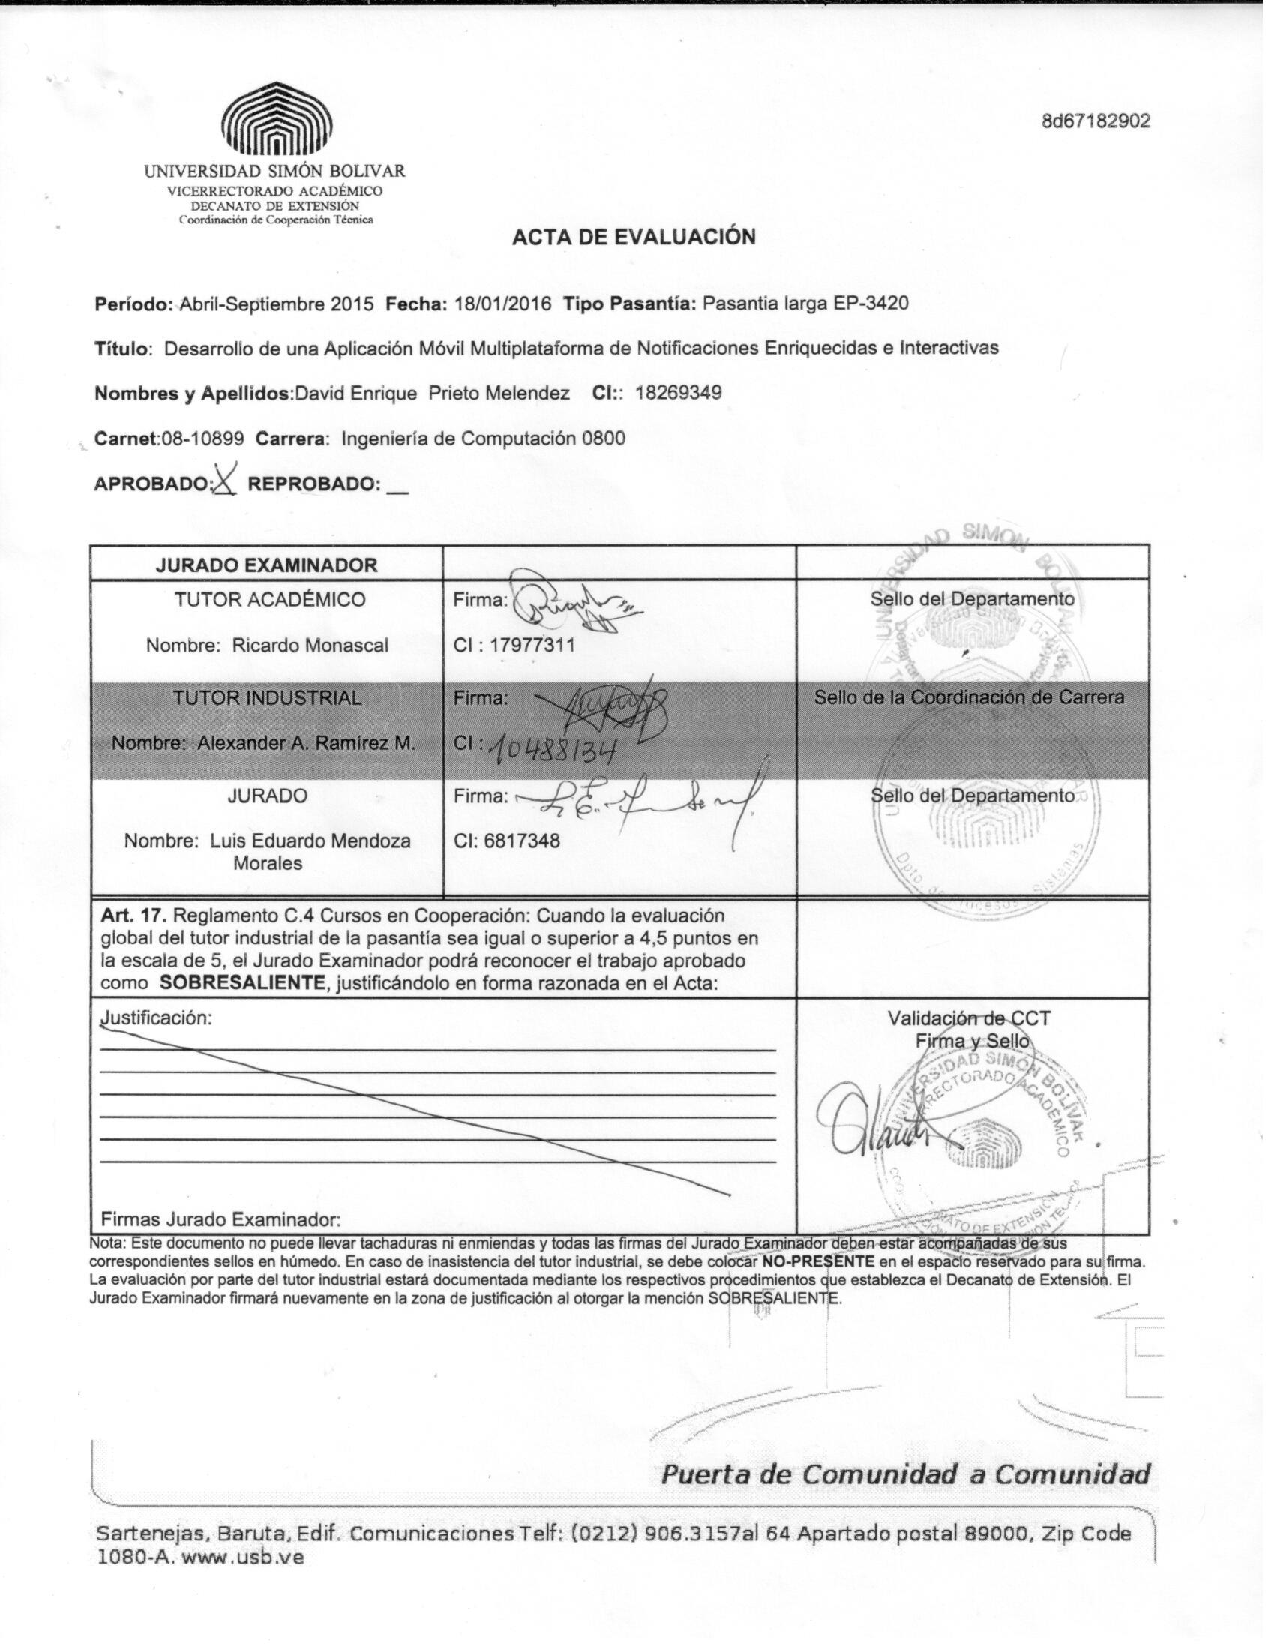
\includepdf[pages={1}]{ActaEvaluacionSELLADA.pdf}

\setcounter{secnumdepth}{3}
\setcounter{tocdepth}{4}

% Define encabezado numeros romanos y como se separan los captiulos y las
% secciones
\addtolength{\headheight}{3pt}
\pagenumbering{roman}
\pagestyle{fancyplain}

\renewcommand{\chaptermark}[1]{\markboth{\chaptername\ \thechapter:\,\ #1}{}}
\renewcommand{\sectionmark}[1]{\markright{\thesection\,\ #1}}

\onehalfspacing

\lhead{}
\chead{}
\rhead{}
\renewcommand{\headrulewidth}{0.0pt}
\lfoot{}
\cfoot{\fancyplain{}{\thepage}}
\rfoot{}

% Cambios de titulos de indices
\renewcommand{\listfigurename}{Índice de Figuras}
\renewcommand{\listtablename}{Índice de Tablas}
\renewcommand{\tablename}{Tabla}
\renewcommand{\contentsname}{Índice General}

% Pagina de resumen
\setcounter{page}{4}
\begin{center}

{\bfseries DESARROLLO APLICACION NOTIFICACIONES+\\}
\bigskip
Por: \\ David Enrique Prieto Melendez\\
\bigskip
\bigskip
{\bf RESUMEN} \pdfbookmark[0]{Resumen}{resumen} % Sets a PDF bookmark for the dedication
\end{center}	

El presente informe describe las actividades realizadas durante el proyecto de pasantía larga, el cual consistió en diseñar y desarrollar un prototipo funcional de la aplicación web de \textit{Notificaciones+} y un prototipo funcional de la aplicación móvil del mismo. Este conjunto de aplicaciones están orientadas a los clientes de bancos, que tengan un dispositivo con la capacidad de desplegar un navegador web, o un dispositivo que funcione bajo las plataformas Android e iOS. Los prototipos funcionales de \textit{Notificaciones+} permiten la recepción de mensajes clasificados de acuerdo a su tipo, que un banco desee mandar a sus clientes. También se permite a los clientes mandar una respuesta al banco según el tipo específico del mensaje, en caso de que el banco requiera una respuesta por parte de sus clientes para una operación.


Para lograr el conjunto de objetivos de \textit{Notificaciones+} fue necesaria la implementación de la lógica de las aplicaciones para el manejo de la recepción y gestión de mensajes provenientes de la plataforma \textit{Synergy Push}. Desde el punto de vista tecnológico se hizo uso de herramientas y tecnologías como JavaScript, AngularJS, Ionic Framework, Node.js. Los resultados de esta pasantía, realizados de acuerdo a la Metodología de Synergy-GB y documentados con artefactos de desarrollo de sistemas implantados en la empresa, incluyen el diseño y desarrollo de \textit{Notificaciones+}, así como la integración adecuado con los servicios web y push de la plataforma \textit{Synergy Push}.

\bigskip
\noindent
PALABRAS CLAVES: IONIC, MULTIPLATAFORMA, PUSH, MENSAJERÍA, WEB.


% Pagina de dedicatoria (opcional)
\pagebreak

%\setcounter{page}{5}

%\vspace*{8cm} 
\pdfbookmark[0]{Dedicatoria}{dedicatoria} % Sets a PDF bookmark for the dedication
\begin{flushright} 
\textit{A mi mismo,}

\textit{por enseñarme a luchar por lo que quiero, apoyarme}


\textit{y darme la fortaleza para seguir adelante.}
\end{flushright}
\newpage


% Pagina de agradecimientos (opcional)
%\setcounter{page}{6}

\chapter*{Agradecimientos
\markboth{Agradecimientos}{Agradecimientos}}
\pdfbookmark[0]{Agradecimientos}{agradecimientos}

\bigskip

Agradezco a Ricardo Monascal, por su disposición a ayudar y por guiarme a lo largo de la pasantía y de toda mi carrera, incluso cuando no tenía tiempo para sí mismo.


A Alejandra Facchin, por tenerme paciencia.


A Marielby Soares, por su constante ayuda y atención, sin tener ninguna razón para hacerlo.


A Miguel Fagundez, por estar siempre dispuesto a ayudarme en este proyecto.


A Ernesto Hernández-Novich, por enseñarme a ver la vida y mi profesión de otra manera.


A Synergy-GB por brindarme la oportunidad y la confianza para desarrollar este proyecto.


A mi perra Miku, por hacerme compañía cuando más lo necesitaba y darme calor en las noches.


Y a todas las personas que han contribuido en mi desarrollo profesional.


% Crea la tabla de contenidos
\tableofcontents

% Crea la lista de cuadros
\listoftables

% Crea la lista de figuras
\listoffigures
%\newpage
\phantomsection
%\setcounter{page}{4}
\chapter*{Lista de Símbolos y Abreviaturas}% Sets a PDF bookmark for the dedication

\vspace{5 mm}
\noindent
\textbf{GB:} Global Business\\
\textbf{API:} Application Programming Interface\\
\textbf{SOAP:} Simple Object Access Protocol\\ 
\textbf{SOA:} Service Oriented Architecture\\ 
\textbf{REST:} Representational State Transfer\\ 
\textbf{HTTP:} Hypertext Transfer Protocol\\ 
\textbf{MVC:} Modelo Vista Controlador (Model–View–Controller)\\ 
\textbf{SPI:} Service Provider Interface\\ 
\textbf{POM:} Project Object Model\\ 
\textbf{JSON:} JavaScript Object Notation\\
\addcontentsline{toc}{chapter}{Lista de Símbolos y Abreviaturas}

% Crea la lista de codigos fuentes
%\lstlistoflistings

\clearpage

% Define encabezado en numeros arabicos  
\pagenumbering{arabic}

\fancyhf{} % Redefine el encabezado 
\lhead{}
\chead{}
\rhead{\fancyplain{}{\thepage}}
\renewcommand{\headrulewidth}{0.0pt}
\lfoot{}
\cfoot{}
\rfoot{}

\onehalfspacing

% Incluye los archivos deseados - El contenido de su proyecto de grado/pasantia larga.
\phantomsection
\addcontentsline{toc}{chapter}{Introducción}
\chapter*{Introducción} \label{sec:Introduccion}
%\pdfbookmark[0]{Introducción}{introduccion} % Sets a PDF bookmark for the dedication

\vspace{5 mm}


Con el pasar de los años, las empresas evolucionan con el fin de ofrecer a sus clientes mejores productos. Synergy-GB es una compañía que desarrolla gran variedad de aplicaciones web y móviles, teniendo como gran parte de su clientela bancos; habiendo desarrollado, entre otras, las aplicaciones móviles bancarias del Banco Banesco y del Banco Mercantil. El mercado bancario es cada día más exigente y se encuentra en constante necesidad de innovaciones para ser más atractivo a sus clientes y poder ofrecer mejor calidad de servicios. En un inicio se ofrecían servicios de banca común (como la capacidad de consulta de saldos y balances de las cuentas de cada usuario del banco), sin la necesidad de una computadora de escritorio o portátil sino con el simple uso de un dispositivo móvil o Smartphone. Sin embargo, con el paso del tiempo y poco a poco, lo que fue bautizado como banca móvil fue expandiéndose, tomando en cuenta operaciones cada vez más complejas, como la disposición de saldos y movimientos de las tarjetas de crédito. De esta manera se hizo evidente que la mayoría de las operaciones bancarias, que en un principio debían seguir un proceso tedioso directamente en los bancos para poder realizarse, ahora pueden realizarse en el móvil de forma rápida y cómoda.


El proyecto de pasantía descrito en el siguiente informe tiene, entre sus propósitos, innovar sobre un tema en particular de la banca móvil: las notificaciones bancarias, dado que es un tema con el cual los bancos ya han experimentado explotar en diversas vías y se ha vuelto engorroso tanto para ellos como para sus clientes, ya que algunas notificaciones son enviadas por correo electrónico y otras por SMS y los clientes tienen distintos tipos de notificaciones en distintos medios y no llevan un registro adecuado. Mediante el desarrollo de una aplicación móvil y una aplicación web se ofrece una solución de unificación de notificaciones. El siguiente informe mostrará no solo como se puede ofrecer un buzón digital de notificaciones bancarias, sino la expansión de la comunicación entre un banco y sus clientes, así sea por motivos de seguridad o informativos, que permita al usuario escoger opciones y cominicarse de vuelta con el banco de manera sencilla e inmediata. Todo esto en pro de que el usuario se vea beneficiado con toda esta información disponible de una forma sencilla y cómoda, en un solo lugar. De esta manera Synergy-GB podrá ofrecer algo innovador que facilite la vida de su clientela. El objetivo general del proyecto de pasantía, planteado por la empresa y logrado a lo largo de su desarrollo, fue: “Desarrollar la aplicación web y la aplicación móvil multiplataforma en PhoneGap, Ionic Framework y Angular.js para recibir notificaciones y alertas enriquecidas e interactivas”. Para alcanzarlo se plantearon los siguientes objetivos específicos:


\begin{itemize}[noitemsep,nolistsep]
\item Diseñar la arquitectura de la aplicación basándose en la arquitectura de Synergy Push.
\item Desarrollar la integración con Synergy Push.
\item Desarrollar el módulo envío de notificaciones.
\item Desarrollar el módulo de gestión de contenido y respuestas de los usuarios.
\item Desarrollar la aplicación web tomando en cuenta las mejores prácticas del diseño web 2.0.
\item Desarrollar la aplicación móvil multiplataforma, tomando en cuenta las mejores prácticas del desarrollo para dispositivos móviles y utilizando la plataforma PhoneGap, ionic, angularjs y nodejs.
\end{itemize}


Este informe presenta los resultados de la investigación, diseño e implementación de \textit{Notificaciones+}. Se explicarán las diferentes fases del desarrollo del mismo y el proceso de transformación del concepto abstracto inicial en un prototipo funcional, junto con las decisiones de diseño tomadas a lo largo del desarrollo.


El informe está organizado de la siguiente manera: en el capítulo 1 se provee una visión general de Synergy-GB para familiarizar al lector con la empresa. En el capítulo 2 se presentan algunos conceptos teóricos fundamentales. En el capítulo 3 se describen las herramientas tecnológicas utilizadas en el desarrollo del prototipo. En el capítulo 4 se describe la metodología de Synergy-GB, utilizada en la pasantía.  El capítulo 5 presenta el proceso completo de diseño e implementación del canal Web de Banca. El capítulo 6 señala los retos enfrentados durante el desarrollo. Luego, se exponen las conclusiones y algunas recomendaciones derivadas del proceso de investigación y desarrollo, seguidas de las referencias bibliográficas y el glosario. Finalmente, en los Apéndices se presentan los artefactos que se realizaron a lo largo de este proyecto de pasantía.



% Entorno empresarial.
\chapter{Entorno Empresarial} \label{chap:Entorno Empresarial}

\vspace{5 mm}


En esta sección se describe el ambiente organizacional en el que se desarrolló el proyecto de pasantía de la aplicación web y móvil de \textit{Notificaciones+}. Se presenta la empresa Synergy-GB, sus valores, objetivos y estructura organizativa.


Synergy-GB es una empresa perteneciente al grupo Corporativo SYNERGY-GB Corporation, dedicada al desarrollo y comercialización de productos bajo Tecnologías de Información. Estudia las tendencias a nivel de aplicaciones corporativas actuales a las empresas, a fin de ofrecer soluciones en sus mercados que estén en línea con las prioridades gerenciales y de negocio del mundo actual.

La cartera de aplicaciones va desde Soluciones Integrales Sistémicas que resuelven una problemática compleja en la empresa, hasta Soluciones Puntuales Departamentales que resuelven problemas específicos en procesos de negocio donde se ha perdido el control gerencial  \cite{ESGB0}.


La misión de la empresa, según revela su portal web es “crear, desarrollar y apoyar modelos de negocio que mejoren la competitividad y productividad de sus clientes”  \cite{ESGB0}. 
La visión de Synergy-GB es “Convertir a Synergy-GB en una organización de alcance hispanoamericano, que combine en forma creativa, ideas, talento, tecnología, visión empresarial, innovación y excelencia en el servicio”  \cite{ESGB0}. 
Los valores que definen a Synergy-GB como empresa son \cite{ESGB0}:
\begin{itemize}[noitemsep,nolistsep]
\item Compromiso con la Calidad.
\item Compromiso con la Satisfacción al Cliente.
\item Compromiso con la Generación de un Legado.
\item Sentido de Propiedad.
\item Sentido Emprendedor.
\item Integridad y Honestidad.
\item Orientación a Resultados.
\item Compromiso con la Innovación y el Desarrollo de nuevas ideas.
\item Proactividad.
\item Trabajo en Equipo.
\item Socialmente Responsables.
\item Comercialmente Astutos.
\item Diversión como elemento catalizador.
\end{itemize}

En la Figura ~\ref{fig:estsyn} se presenta la estructura organizativa de la empresa \cite{ESGB1}. El desarrollador ocupó el puesto de pasante en el área de aplicaciones.

\begin{figure}[ht]
  \centering
  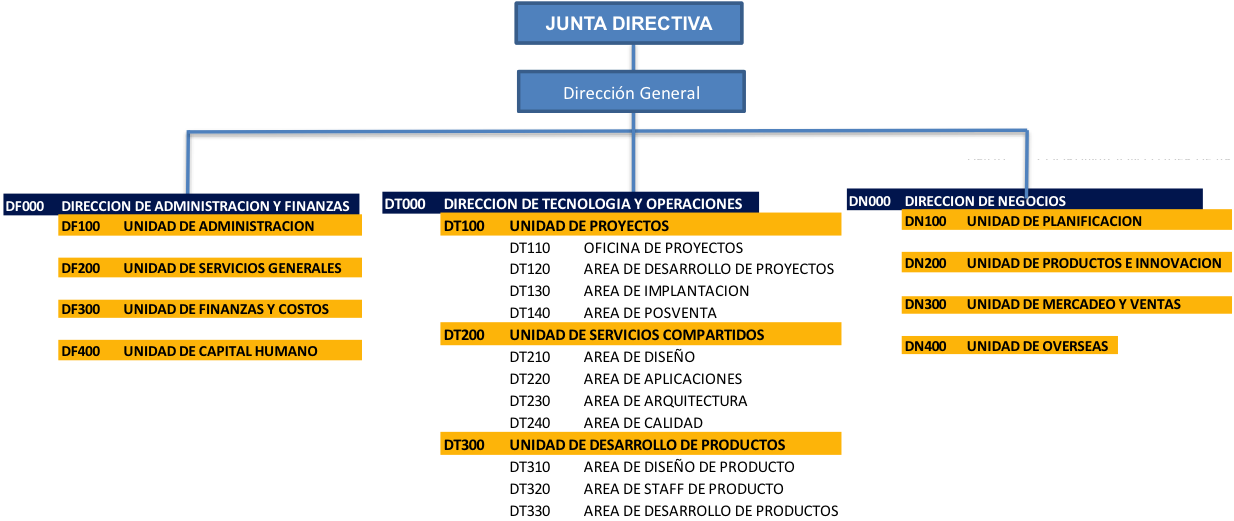
\includegraphics[scale=0.6,type=png,ext=.png,read=.png,angle=0,origin=c]{imagenes/estructurasynergy}
  \caption{Estructura Organizativa de Synergy-GB, C.A.}
  \label{fig:estsyn}
\end{figure}


Entre las áreas de la empresa, las siguientes son las más relevantes \cite{ESGB2}:
\begin{itemize}[noitemsep,nolistsep]
\item {Oficina de proyectos:} 

Se ocupa de centralizar y coordinar la dirección de proyectos. 

\item {Diseño e Imagen:}

Encargada de realizar los diseños que proyecten la imagen Corporativa de la empresa y además de los diseños adecuados a la imagen de cada cliente de acuerdo a los objetivos de cada proyecto. 

\item {Posventa:}

Gestiona la relación con los clientes después que se implantan las soluciones, productos o servicios que ofrece la empresa, además se encarga de gestionar la atención de incidencias, errores, fallas, reclamos, mantenimiento, actualizaciones o requerimientos de nuestros clientes. 
 
\item {Calidad e Implantación:}
 
Se encarga de velar por la calidad de los servicios que ofrece la empresa de forma integral, desde los procesos, la metodología de trabajo y ejecución de proyectos hasta las encuestas de satisfacción después que se entrega una solución.

\item {Administración:}

Gerencia los procesos relacionados con la gestión de la información financiera y laboral de la empresa.

\item {Aplicaciones:}

Se encarga de gerenciar la fábrica de proyectos y productos en particular, la asignación del Talento a los diversos proyectos, productos o servicios de fábrica, implantación o posventa. El área desarrolla los Skills técnicos para el desarrollo de aplicaciones Móviles o Web así como la Integración de plataformas con foco continuo en la Innovación tecnológica y la entrega de soluciones de vanguardia.

\item {Unidad Comercial:}

Es la encargada de la gestión de ventas y relacionamiento con clientes y prospectos, coordinando las actividades que permitan llevar una oportunidad desde su detección (proactiva o reactivamente), hasta la presentación y negociación del cierre de la misma en el marco de una metodología que garantice una alta probabilidad de éxito.  

\item {Unidad Productos:} 

Es la máxima responsable de la gestión de productos de la organización. Su responsabilidad abarca desde la concepción de los productos hasta su maduración y consolidación. Gestiona los productos a lo largo de todo su ciclo de vida ayudando en cada momento a definir las estrategias comerciales y de mercadeo a seguir. 



\end{itemize}


 % Marco Teorico.
\chapter{Marco Teórico} \label{chap:Marco Teorico}

\vspace{5 mm}

En este capítulo se describen los conceptos estudiados para elaborar el proyecto. Al mismo tiempo, proporciona un conocimiento de la teoría que le da significado a las soluciones encontradas durante el desarrollo del proyecto.

\section{Notificación Push} \label{sect:Notificacion Push}

Las Notificaciones Push son mensajes que se envían de forma directa a dispositivos móviles (Smartphones y/o tablets) con sistema operativo iOS, Android, Blackberry o Windows Phone. La recepción por parte de los dispositivos no está garantizada. \cite{MTPUSH}.  

\section{Servicio web} \label{sect:Servicio web}

Los servicios web son un conjunto de protocolos y estándares definidos que sirven para intercambiar datos por medio de comunicaciones remotas en redes como Internet, permitiendo la interoperabilidad entre aplicaciones desarrolladas en distintos lenguajes de programación o ejecutadas en distintas plataformas \cite{MTREST}. 

La definición de los servicios web se basa en una serie de especificaciones y estándares aceptados por la mayoría como SOAP (Simple Object Access Protocol), WSDL (Web Services Description Language) y UDDI (Universal Description, Discovery and Integration), basados en XML (Extensible Markup Language). Sin embargo también existen otros protocolos de servicios web como REST (Representational State Transfer, descrito en la sección ~\ref{sect:Transferencia de estado representacional (REST)}) y distintos formatos de intercambio de datos y mensajes adicionales a XML como JSON (JavaScript Object Notation) \cite{MTREST}.

\section{Transferencia de Estado Representacional (REST)} \label{sect:Transferencia de estado representacional (REST)}

La Transferencia de Estado Representacional (REST, por sus siglas en inglés), es un estilo arquitectónico para sistemas distribuidos. Los sistemas REST normalmente se basan en el protocolo HTTP para definir todas las operaciones que se pueden realizar. Estas operaciones aplican sobre recursos, los cuales son entidades semánticas que representan un objeto o concepto bien definido dentro del sistema\cite{MTREST}.

Entre los fundamentos de REST se encuentran \cite{MTREST}:
\begin{itemize}[noitemsep,nolistsep]
\item Está basado en un protocolo cliente/servidor sin estado.
\item Posee un conjunto de operaciones bien definidas que se aplican a todos los recursos de información.
\item Ofrece una sintaxis uniforme para identificar los recursos.
\end{itemize}

\section{Arquitectura de tres capas} \label{sect:Arquitectura de tres capas}
La arquitectura de tres capas es una arquitectura cliente/servidor compuesta por la capas de datos, aplicación y presentación \cite{MTATC}.
La capa de datos es responsable de almacenar, en un servidor de datos dedicado, información de la configuración y datos del negocio. La capa de aplicación, también denominada capa lógica, de negocio o servidor de aplicación, controla toda la funcionalidad, y provee procesos lógicos de negocio y acceso a los datos. La capa de presentación ofrece a los usuarios la lógica de presentación; es decir, el acceso a la información a través de una interfaz de usuario \cite{MTATC2}.
La utilización de una arquitectura de tres capas en el desarrollo de sistemas, en base a las características previamente expuestas, ofrece las siguientes ventajas:
\begin{itemize}[noitemsep,nolistsep]
\item Brinda capacidad de reutilización de código y funcionalidades, especialmente en la capa intermedia o de negocios.
\item Provee independencia entre capas y un mínimo impacto a la hora de realizar cambios. 
\item Facilita del mantenimiento y mejora del sistema.
La arquitectura de tres capas tiene su origen a principio de los años noventa en vista de la necesidad de superar las limitaciones inherentes en una arquitectura de dos capas. La utilización de tres capas establece un diseño efectivo cuando se necesita un esquema de tipo cliente/servidor o de datos distribuidos mediante la provisión de un mejor desempeño, flexibilidad, mantenimiento facilitado, reutilización y escalabilidad \cite{MTATC3}.
\end{itemize}

\section{Patrón MVC (Modelo-Vista-Controlador)} \label{sect:Patron MVC}
Antes de proporcionar una definición de Modelo-Vista-Controlador, hay que definir un patrón de diseño. “Los patrones de diseño son el esqueleto de las soluciones a problemas comunes en el desarrollo de \textit{software}” \cite{MTMVC1}. 

MVC es un patrón de diseño de \textit{software} que separa el código fuente en tres capas o componentes con funciones muy especiales \cite{MTMVC2}: 
\begin{itemize}[noitemsep,nolistsep]
\item Modelo: administra el comportamiento y los datos del dominio de la aplicación (es decir, maneja la lógica del negocio), responde las solicitudes de información acerca de su estado (provenientes, generalmente, de la vista), mientras que manipula los datos a petición del controlador. 
\item Controlador: Es la capa que interpreta eventos (usualmente acciones del usuario), informando a la vista y al modelo sobre los cambios necesarios para generar una respuesta. De manera más precisa, el controlador informa al modelo sobre cambios en la información, y a la vista sobre la manera en la que deben presentarse los datos provenientes del modelo. 
\item Vista: Es la sección encargada de “presentar” el modelo (lógica del negocio). Esta capa se centra en la interacción directa con el usuario del sistema o aplicación. 
\end{itemize}

\section{Software as a Service} \label{sect:Software as a Service}

SaaS es un modelo de entrega de \textit{software} en el que el fabricante es responsable de la operación técnica diaria del \textit{software} proporcionado a los clientes (incluyendo el mantenimiento y soporte), mientras los clientes disfrutan de los beneficios del \textit{software} desde ubicaciones remotas \cite{MTSAAS}.
La aparición de SaaS como un mecanismo efectivo de entrega de \textit{software} crea una oportunidad para los departamentos de Tecnología de la Información (IT por sus siglas en inglés) de cambiar su enfoque de despliegue y soporte de aplicaciones para la gestión de los servicios que ofrecen éstas aplicaciones \cite{MTSAAS2}.

\section{WEB 2.0} \label{sect:WEB 2.0}

La web 2.0 es la revolución de los negocios en la industria de la computación causada por el movimiento de Internet como una plataforma, y un intento por entender las reglas para el éxito de esa plataforma. La principal de esas reglas es la siguiente: construir aplicaciones que aprovechen los efectos de la red para que mejoren a medida que la gente las utiliza \cite{MTSAAS}.
La web 2.0 generalmente se refiere a un conjunto de patrones sociales, arquitectónicos y de diseño que resultan en la migración masiva de los negocios al Internet como plataforma. Estos patrones se enfocan en los modelos de interacción entre comunidades, personas, computadoras y \textit{software}. En esencia, las filosofías y tecnologías de la web 2.0, permiten que la interacción, a niveles sin precedentes, ayude a promover la innovación, la velocidad y la sencillez; por ejemplo: aprovechar la inteligencia colectiva de la gente, descubrir y aprovechar las comunidades de interes y conectar a las personas entre si y a la información relevante de manera más eficiente \cite{MTSAAS}.

\section{Single Page Application (SPA)} \label{sect:Single Page Application} 

Una \textit{Single-Page-Application} (o aplicación de una sola página), es una aplicación o sitio web que maneja una sola página web, con el objetivo de proveer una experiencia de uso más fluida al usuario (similar a las aplicaciones de escritorio).
En una SPA se recupera todo el código necesario para cargar una sola página, o las fuentes necesarias se cargan dinámicamente y se agregan a la página conforme se necesiten. La página no es refrescada nunca, aunque ciertas tecnologías dan la ilusión de que se está navegando en más de una página. Muchas veces interactuar con una SPA involucra comunicarse con servicios web \cite{MTSPA}.

%\end{itemize} 


 % Marco Teorico.
\chapter{Marco Tecnológico} \label{chap:Marco Tecnologico}

\vspace{5 mm}

En este capítulo se presentan las características principales de las herramientas tecnológicas seleccionadas para el desarrollo del proyecto de pasantía. 

\section{HTML (HyperText Markup Language)} \label{sect:HTML}
HTML (HyperText Markup Language) es un lenguaje de marcado para describir documentos web mediante etiquetas. Consiste en una serie de etiquetas para definir la estructura de la página y mediante ella se pueden definir textos imágenes y otros \cite{HTML}. 

\section{CSS (Cascading Style Sheets)} \label{sect:CSS}
CSS (Cascading Style Sheets), es un formato que permite definir cómo mostrar los elementos HTML, permite separar la estructura del documento de su estilo y los detalles propios del formato del mismo. Se pueden definir estos estilos y formatos en el mismo documento HTML o en un documento de formato .css aparte \cite{CSS}. 

\section{JavaScript} \label{sect:JavaScript}
JavaScript es un lenguaje de programación interpretado que permite darle lógica al marcado (HTML) y al estilo (CSS) de las páginas web. Forma parte de las herramientas que tiene un navegador web para poder mostrar una página web dinámica \cite{JS0}.

\section{JSON} \label{sect:JSON}
JSON, acrómimo de JavaScript Object Notation, es formato de intercambio de datos liviano basado en un subconjunto del lenguaje de programación JavaScript. Este formato posee dos estructuras básicas: pares nombre/valor y listas ordenadas de valores, por lo cual es entendible con facilidad por los humanos y simple de interpretar o generar para las máquinas. Representa una de las principales alternativas al XML \cite{JSON}. 

\section{Node.js} \label{sect:Node}
Node.js es una plataforma construida sobre V8 JavaScript Runtime, el motor de JavaScript de código abierto de Google (V8 JavaScript Engine, 2008), para construir aplicaciones de red escalables. Node.js utiliza un manejador de eventos, un modelo de I/O no bloqueante que lo hace ligero y eficiente, ideal para aplicaciones de tiempo real que manejan gran cantidad de datos y que se ejecutan a través de dispositivos distribuidos \cite{NODE}. 

\section{Grunt} \label{sect:Grunt}
Es un intérprete (y ejecutor) de tareas de JavaScript que se usa para la automatización de tareas repetitivas en el desarrollo de aplicaciones web para que el programador pueda concentrarse en las áreas relevantes del desarrollo. Entre estas tareas se encuentran compilación, minificación y pruebas unitarias \cite{GRUNT}.

\section{PhoneGap} \label{sect:PhoneGap}
Phonegap es una solución de \textit{software} libre para construir aplicaciones móviles multiplataformas usando tecnologías web estándar, como HTML, CSS y JavaScript \cite{PHGAP}. Además permite el acceso a los widgets de los móviles, tales como el acceso a los sensores del dispositivo, cámara, acelerómetro y otros a través de su API. Entre los beneficios de Phonegap están:
\begin{itemize}[noitemsep,nolistsep]
\item Incrementa la velocidad de desarrollo de aplicaciones móviles. 
\item Permite que con un sólo desarrollo, las aplicaciones puedan ser multiplataforma.
\item No es necesario saber desarrollar en cada uno de los lenguajes (de cada plataforma móvil) para desarrollar la aplicación. Sólo es necesario tener conocimientos de programación web y tener en cuenta el API de PhoneGap.
\end{itemize}

\section{Cordova} \label{sect:Cordova}
Es la plataforma en la cual está basada PhoneGap. Permite el uso de las funciones de los dispositivos móviles, sin importar a que plataforma pertenecen (Android, iOS, Windows Phone, BlackBerryOS). Por esa razón, la mayoría de las funciones y comandos son idénticas, y muchas documentaciones se refieren a PhoneGap y Cordova como la misma plataforma \cite{CORDOVA}.

\section{AngularJS} \label{sect:AngularJS}
Es un framework de \textit{software} libre mantenido por Google y la comunidad, que ayuda a la creación de aplicaciones de página única (SPA) usando HTML, CSS y JavaScript. Logra simplificar el desarrollo extendiendo el vocabulario HTML. Es extensible y su integración es sencilla; cada característica puede ser sobrescrita o modificada según se requiera \cite{ANGULAR}.

\section{Ionic Framework} \label{sect:Ionic Framework}
Ionic es un framework de desarrollo de aplicaciones usando HTML5 que contribuye a diseñar aplicaciones móviles que permitan dar la sensación de ser nativas en cuanto a su desempeño \cite{IONIC}. Se apoya en Phonegap para poder crear la aplicación y potencia así la velocidad de desarrollo de la misma. Además, viene integrado con AngularJS. 


 % Marco Metodologico.
\chapter{Marco Metodológico} \label{chap:Marco Metodologico}

\vspace{5 mm}

En este capítulo se describe la metodología utilizada para el desarrollo del proyecto, la cual es una versión “ágil” de OpenUp y se denomina Metodología de Proyectos Synergy-GB; además, se describe brevemente el marco de trabajo utilizado para la gestión del desarrollo del prototipo funcional tanto de la aplicación web como de la aplicación móvil de Notificaciones+.


Para efectos de este proyecto de pasantía, son muchos los artefactos que se describen en la Metodología de Proyectos Synergy-GB que no son aplicables al mismo ya que consisten en entregables directos a algún cliente, y en este caso el cliente es la misma empresa.


\section{Metodología de Proyectos Synergy-GB} \label{sect:Metodologia Synergy}
Describe las herramientas y artefactos que facilitan la comunicación y alineación tanto interna  (entre los integrantes del equipo de trabajo) como externa (de Synergy-GB hacia el cliente) en cuanto al seguimiento y progreso de los proyectos \cite{MMSynergy}. 

En la Figura ~\ref{fig:metosyn} se muestran las etapas en las cuales de divide la Metodología de Proyectos Synergy-GB \cite{MMSynergy}.

\begin{figure}
  \centering
  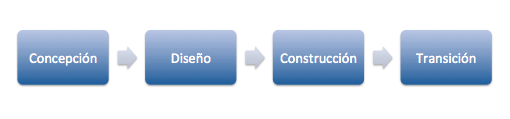
\includegraphics[scale=0.7,type=png,ext=.png,read=.png,angle=0,origin=c]{imagenes/metodologiasynergy}
  \caption{Etapas de la Metodología de Proyectos Synergy-GB. 
(Synergy-GB Área de Calidad).}
  \label{fig:metosyn}
\end{figure}

\subsection{Concepción}
En esta etapa se definen los documentos de requerimientos y el acuerdo con el cliente, acerca de los entregables que se deben realizar en el proceso de ejecución del proyecto. Los involucrados en esta etapa son el líder de proyecto (Synergy-GB) y el cliente, y la persona responsable de cada una de las actividades es el líder de proyecto \cite{MMSynergy}.

\subsection{Diseño}
En esta etapa se construyen los diseños de funcionalidad y servicios que se requieren para la etapa de construcción del producto. Las personas involucradas en esta etapa de la metodología son: líder de proyecto, arquitecto, diseñador, integración y calidad \cite{MMSynergy}.

\subsection{Construcción}
En esta etapa del proyecto, se realiza el desarrollo de la aplicación por parte del equipo del proyecto (Integración, Ux, Móvil, Web) encargado en el área correspondiente; en este caso, el encargado designado por la empresa es el pasante. Para su gestión, se utilizó el marco de trabajo Scrum. La fase de dividió en tres (3) iteraciones, de un mes de duración cada una. En el capítulo 5 se describirá con más detalle las actividades realizadas \cite{MMSynergy}.

\subsection{Transición}
La etapa de transición representa un punto de validación y cierre para el proyecto. Es en este momento cuando se realizan todas las pruebas sobre los distintos componentes de la solución, determinando que su funcionamiento es el correcto y su presentación cumple con los diseños elaborados en tempranas etapas. Por lo tanto,  se llevan a cabo las pruebas de estrés por parte del equipo de Integración y Ux, y luego las pruebas de los servicios e integrales por parte del equipo de calidad involucrado en el proyecto \cite{MMSynergy}.

\section{Scrum} \label{sect:Scrum}
Es un marco de trabajo dentro del cual las personas pueden  afrontar complejos problemas adaptativos, a la vez que entregan productos del máximo valor posible de forma proactiva y creativa. No es una técnica de construcción de productos, sino simplemente un marco de trabajo flexible en donde se pueden emplear diversas técnicas o procesos \cite{MMSCRM}. 

Scrum se fundamenta en la teoría empírica de procesos, en donde se asegura que el conocimiento procede de la experiencia y de tomar decisiones basándose en lo que se conoce. Scrum emplea una aproximación iterativa e incremental para optimizar la predictibilidad y controlar el riesgo \cite{MMSCRM}.

Al fundamentarse en la teoría empírica de procesos, Scrum debe soportarse sobre los siguientes tres pilares: transparencia, inspección y adaptación \cite{MMSCRM}.

\subsection{El equipo Scrum (Scrum team)}
El Scrum team está conformado por el dueño del producto, el equipo de desarrollo y el Scrum master (jefe del Scrum o facilitador). A continuación, se especifican las responsabilidades de cada uno de los integrantes del equipo \cite{MMSCRM}:

\begin{itemize}[noitemsep,nolistsep]
\item {Dueño del producto (product owner):}

Es el encargado de maximizar el valor del producto y del trabajo del equipo de desarrollo; a su vez, es la única persona que puede gestionar el product backlog (pila del  producto, más adelante se especificará qué es exactamente). Es el responsable del producto desde un punto de vista comercial o de negocio.
\item {Equipo de desarrollo:}

Es el equipo de trabajo que participa en un Sprint dentro de la práctica Scrum. Realiza las tareas de diseño y desarrollo de \textit{software}. Desde un punto de vista más general, son los profesionales que realizan los incrementos de un producto, posiblemente funcional, al final de cada sprint. Sólo los integrantes del equipo de desarrollo están autorizados para realizar los incrementos del producto.
\item {Scrum master:}

Tiene como responsabilidad asegurar que Scrum, como marco de trabajo, es entendido y llevado a cabo correctamente. Es un líder servil que se encuentra a la orden de todo el Scrum team. Por otra parte, el Scrum master es aquel puente entre agentes externos al Scrum team y este último.
\end{itemize}

\subsection{El Sprint}
El núcleo de Scrum es el Sprint, un período de tiempo de a lo sumo un mes durante el cual se crea un incremento de producto utilizable y potencialmente entregable. Cada nuevo sprint comienza inmediatamente después de la finalización del Sprint anterior \cite{MMSCRM}.

Para asegurar el correcto funcionamiento del sprint, deben seguirse las siguientes normas \cite{MMSCRM}:
\begin{itemize}[noitemsep,nolistsep]
\item No se realizan cambios que afectarían al objetivo del sprint.
\item La composición del Equipo de Desarrollo se mantiene constante.
\item	Los objetivos de calidad no disminuyen.
\item	El alcance puede ser clarificado y renegociado entre el Dueño de Producto y el Equipo de Desarrollo a medida que se va aprendiendo más.
\end{itemize}

Los Sprints están compuestos por la reunión de planificación del sprint (Sprint Planning Meeting), los Scrums diarios (Daily Scrums), el trabajo de desarrollo, la revisión del sprint (Sprint review), y la retrospectiva del sprint (Sprint Retrospective) \cite{MMSCRM}:

\begin{itemize}[noitemsep,nolistsep]
\item {Reunión de Planificación del Sprint (Sprint Planning Meeting):}

El trabajo a realizar durante el Sprint es planificado en la Reunión de Planificación de Sprint. Este plan es creado mediante el trabajo colaborativo del Equipo Scrum al completo.
La Reunión de Planificación de Sprint consta de dos partes, cada una de ellas da respuesta a las siguientes preguntas, respectivamente: ¿Qué será entregado en el Incremento resultante del Sprint que comienza? ¿Cómo se conseguirá hacer el trabajo necesario para conseguir el Incremento?
\item {Scrum Diarios (Daily Scrums):}

Es una reunión de máximo 15 minutos, para que el Equipo de Desarrollo sincronice sus actividades y cree un plan para las siguientes 24 horas. Esto se lleva a cabo inspeccionando el trabajo avanzado desde el último Scrum Diario y haciendo una predicción acerca del trabajo que podría ser completado antes del siguiente. 
\item {Revisión del Sprint (Sprint Review):}

Al final del Sprint se lleva a cabo una Revisión de Sprint, para inspeccionar el Incremento y adaptar la Pila de Producto si fuese necesario. Durante la Revisión de Sprint, el Equipo Scrum y los interesados colaboran acerca de lo que se ha hecho durante el Sprint.
\item {Retrospectiva del Sprint (Sprint Retrospective):}

La Retrospectiva de Sprint es una oportunidad para el Equipo Scrum de inspeccionarse a sí mismo, y crear un plan de mejoras que sean abordadas durante el siguiente Sprint.
\end{itemize}

\subsection{Artefactos}
Los artefactos de Scrum representan trabajo o valor en diversas formas que son útiles para proporcionar transparencia y oportunidades para la inspección y adaptación. Los artefactos definidos por Scrum, están específicamente diseñados para maximizar la transparencia de la información clave, que es necesaria para asegurar que los Equipos Scrum tengan éxito al entregar un Incremento \cite{MMSCRM}:
\begin{itemize}[noitemsep,nolistsep]
\item {Pila de Producto (Product Backlog):}

La Pila de Producto es una lista ordenada de todo lo que podría ser necesario en el producto, y es la única fuente de requerimientos para cualquier cambio a  realizarse en el producto. El Dueño de Producto (Product Owner) es el responsable de la Pila de Producto, incluyendo su contenido, disponibilidad y ordenación.
\item {Pila de Sprint (Sprint Backlog):}

La Pila de Sprint es el conjunto de elementos de la Pila de Producto seleccionados para el Sprint, más un plan para entregar el Incremento de producto y conseguir el Objetivo del Sprint. \\
\end{itemize}
Para los efectos de esta pasantía, el dueño del producto fue Alexander Ramírez. El scrum master fue Ana Dávila y el desarrollador fue el pasante designado por la empresa, supervisado por el líder del área de movilidad Gabriel Vega.

Se desarrollaron los siguientes documentos entregables desde el punto de vista de un proyecto de \textit{software}, los cuales a su vez, representan la documentación del sistema obtenido como resultado de la pasantía: Documento de Arquitectura de Software y Documento de Especificación Funcional.


\chapter{Desarrollo de la Aplicación}\label{chapter:Desarrollo de la Aplicacion}

Este capítulo describe las actividades realizadas en la concepción, diseño, construcción y transición del prototipo de la aplicación web y de la aplicación móvil de Notificaciones+. 
Está dividido en secciones, cada una de ellas representando una fase de la metodología adoptada, descrita en el capítulo anterior.

\section{Concepción} \label{sect:Concepcion}
El objetivo de esta fase consistió en recolectar la información necesaria para levantar los requerimientos del cliente para las aplicaciones a desarrollar. Por este motivo se realizaron reuniones periódicas con el mismo para determinar detalladamente dichos requerimientos y definir las características que tanto la aplicación web, como la aplicación móvil de Notificaciones+ debería poseer.
Esta fase tuvo una duración de 2 semanas, y se realizaron las siguientes actividades:
\smallskip
\begin{itemize}[noitemsep,nolistsep]
  \item Familiarización con la empresa y el entorno laboral.
  \item Investigación sobre las prácticas de la empresa.
  \item Levantamiento de requerimientos funcionales y no funcionales.
  \item Identificación y mitigación de riesgos que puedan afectar el desarrollo del sistema.
  \item Investigación general de herramientas disponibles para ambas aplicaciones (Web y Móvil)
  \item Investiagación de la plataforma Synergy Push.
\end{itemize}
\bigskip

En esta etapa del desarrollo, se inició el documento de especificación funcional y el documento de Arquitectura de Software de Notificaciones+ para Synergy-GB, el cual se refinó en repetidas oportunidades de acuerdo a las solicitudes que el cliente realizó (ver Apéndice B, el cual incluye los requerimientos).

\subsection{Requerimientos}
La lista de requerimientos se realizó de acuerdo al plan de trabajo y a varias reuniones con el cliente para aclarar todo el objetivo de ambas aplicaciones. En la Tabla ~\ref{table:ReqFunc} se presenta un resumen de los requerimientos funcionales de la aplicación web y de la aplicación móvil de Notificaciones+ (véase el Apéndice B para más información).

\begin{table}[H]
%\centering 
\begin{tabular}{| p{6cm} | p{10cm} |}
\hline 
\bfseries \footnotesize {Requerimiento} & \bfseries \footnotesize {Descripción} \\ 
\hline 
\bfseries 
  \footnotesize {Gestionar sesión} &
  \footnotesize Un usuario debe poder iniciar sesión luego de autenticar sus credenciales y cerrar una sesión previamente iniciada. \\ \hline 
\bfseries 
  \footnotesize {Permitir registro} & 
  \footnotesize Un usuario debe poder registrarse desde su dispositivo móvil a la plataforma Synergy Push Services para poder luego iniciar sesión y usar la plataforma. \\ \hline 
\bfseries 
  \footnotesize {Recibir Notificación Push} & 
  \footnotesize El dispositivo del usuario debe poder recibir automáticamente notificaciones Push provenientes de la plataforma Synergy Push Services, una vez el usuario haya iniciado sesión. \\ \hline 
\bfseries \footnotesize {Recibir y Abrir Mensajes Completos} & \footnotesize Un usuario debe poder seleccionar una notificación de su buzón y abrirla para ver todo su contenido. \\ \hline 
\bfseries 
  \footnotesize {Devolver respuesta de una o dos opciones a mensajes que lo requieran} & 
  \footnotesize Un usuario debe poder seleccionar una opción de respuesta a mensajes que requieran esta acción por parte del usuario, como alertas de seguridad interactiva y notificaciones de operaciones bancarias. \\ \hline 
\bfseries 
  \footnotesize {Compartir Mensaje} & 
  \footnotesize Un usuario debe poder compartir desde el buzón y la vista de detalles, un mensaje a través de otras aplicaciones instaladas en su dispositivo móvil. \\ \hline 
\bfseries 
  \footnotesize {Eliminar Mensajes} & 
  \footnotesize Un usuario debe poder eliminar desde el buzón y la vista de detalles, cualquier mensaje que se encuentre allí. \\ \hline 
\end{tabular}
\footnotesize \caption{Resumen de requerimientos funcionales de la aplicación web y de la aplicación móvil de Notificaciones+. Elaboración propia.}
\label{table:ReqFunc}
\end{table}

Un resumen de los requerimientos no funcionales pueden verse en la Tabla ~\ref{table:ReqNoFunc} (pueden consultarse a detalle en el Apéndice B).

\begin{table}[H]
\centering 
\begin{tabular}{| p{3cm} | p{13cm} |}
\hline 
\bfseries \footnotesize {Requerimiento} & \bfseries \footnotesize {Descripción} \\ 
\hline 
\bfseries \footnotesize {Funcionalidad} & \footnotesize El sistema debe cumplir con todas las funcionalidades especificadas en los casos de uso. \\ \hline 
\bfseries \footnotesize {Usabilidad} & \footnotesize El sistema debe ser fácil e intuitivo de usar.  \\ \hline 
\bfseries \footnotesize {Eficiencia} & \footnotesize El sistema debe llevar a cabo todos sus procesos de manera rápida y eficiente.  \\ \hline 
\end{tabular}
\footnotesize \caption{Resumen de requerimientos no funcionales de la aplicación web y de la aplicación móvil de Notificaciones+. Elaboración propia.}
\label{table:ReqNoFunc}
\end{table}


% En la Figura ~\ref{fig:arqbb+} se muestra la especificación del requerimiento “Consultar beneficiarios”, incluyendo las interfaces y estructuras de datos asociadas. En el Apéndice B se encuentra la especificación para cada uno de los requerimientos de la Tabla ~\ref{table:ReqNoFunc} y la Tabla ~\ref{table:ReqFunc}.
% \begin{figure}[ht]
%   \centering
%   \includegraphics[scale=1,type=png,ext=.png,read=.png,angle=0,origin=c]{imagenes/reqespec}
%   \caption{Especificación del Requerimiento Consultar Directorio. Elaboración propia.}
%   \label{fig:arqbb+}
% \end{figure}


\subsection{Riesgos}
El propósito de la lista de riesgos es, en primer lugar, identificar aquellos elementos que pueden afectar negativamente la ejecución del proyecto. Además, permite medir el impacto de cada riesgo y planificar estrategias de mitigación y acciones de contingencia en caso de materializarse alguno de ellos.


Los principales riesgos detectados fueron, en su mayoría, desacuerdos que se originaban por problemas de comunicación entre el desarrollador y el cliente, además de desiciones de diseño que no estaban tomadas y quedaban a improvisación por parte del desarrollador. No obstante, como en este caso el rol de cliente es asumido por la misma empresa Synergy-GB,  las acciones tomadas para mitigar estos riesgos consisten en la realización de reuniones periódicas para mantener los objetivos y requerimientos claros y actualizados.


Probablemente el mayor riesgo sea que la funcionalidad principal de la aplicación, que son la recepción de notificaciones Push, dependían de \textit{software} de terceros, experimental, ajeno a la plataforma Ionic, del cual la compañía nunca había utilizado y no había ninguna garantía que funcionara. 


Otros riesgos que influían en el desarrollo de la aplicación fueron aquellos asociados al cálculo erróneo del tiempo de desarrollo, la pendiente de la curva de aprendizaje de determinadas herramientas utilizadas para el desarrollo del proyecto, en especial AngularJS y su interacción con Cordova, y la subestimación del monto de esfuerzo a ser empleado. Todos estos riesgos fueron mitigados con estrategias de planificación que contemplaran la importancia de los componentes críticos de la aplicación y la complejidad de ciertas herramientas a utilizar.


\subsection{Tecnologías y plataformas de desarrollo}
El proyecto tenía que ser desarrollado bajo ambientes adecuados y hacer uso de tecnologías innovadoras que otorgaran el máximo de beneficios. Para la implementación de la aplicación móvil de Notificaciones+ se utilizaron las herramientas implícitas (frameworks, lenguajes y plataformas) en el desarrollo de una aplicación multiplataforma con Ionic Framework. En orden piramidal: 
\smallskip
\begin{itemize}[noitemsep,nolistsep]
  \item Ionic Framework
  \item AngularJS
  \item JavaScript
  \item HTML5/CSS3
  \item ngCordova
  \item Cordova/Phonegap
  \item iOS/Android
\end{itemize}
\bigskip

Se usó Sublime como editor de texto. Toda la programación se hizo en una PC corriendo Ubuntu 14.10. Se usó un computador MAC OSX para compilar y correr bajo la plataforma iOS debido a las políticas de exclusividad de esa herramienta. También se hizo uso limitado de los respectivos emuladores Android y iOS. Los dispositivos de prueba fueron:
\smallskip
\begin{itemize}[noitemsep,nolistsep]
  \item iPhone 5 con iOS 7
  \item Samsung Galaxy Nexus con Android 4.3 
  \item HTC One S con Android 4.1.1
  \item Huawei con Android 4.4
\end{itemize}
\bigskip 


\subsection{Casos de Uso}

Los Casos de Uso proporcionan uno o más escenarios, los cuales definen la secuencia acciones que debe llevar a cabo el usuario para activar una funcionalidad de las aplicaciones.

El Modelo de Casos de Uso de la aplicación es utilizado con el fin de ilustrar tanto las funcionalidades como la relación entre ellas y los actores que las usan. En la Figura ~\ref{fig:dcuinicial} se puede observar el Diagrama de Casos de Uso inicial, que posteriormente se refinó ya que se ampliaron las funcionaliades y se aclararon ciertos requerimientos de \textit{software}.

En el mismo se observa que se identificaron dos actores. En primer lugar, el Usuario, que se encarga de hacer uso de Notificacones+. Luego, el otro actor es Synergy Push que es la plataforma a la cual se conecta la aplicación para obtener mensajes.


\subsection{Planificación Inicial}

Esta actividad consistió en estimar una planificación para el desarrollo del proyecto: el orden en que serán implementados los Casos de Uso (CU) y el tiempo que debía tomar cada uno de ellos. La Figura ~\ref{fig:dcuinicial} muestra el diagrama de Casos de Uso Inicial que permitío establecer la planificación. 

\begin{figure}[ht]
  \centering
  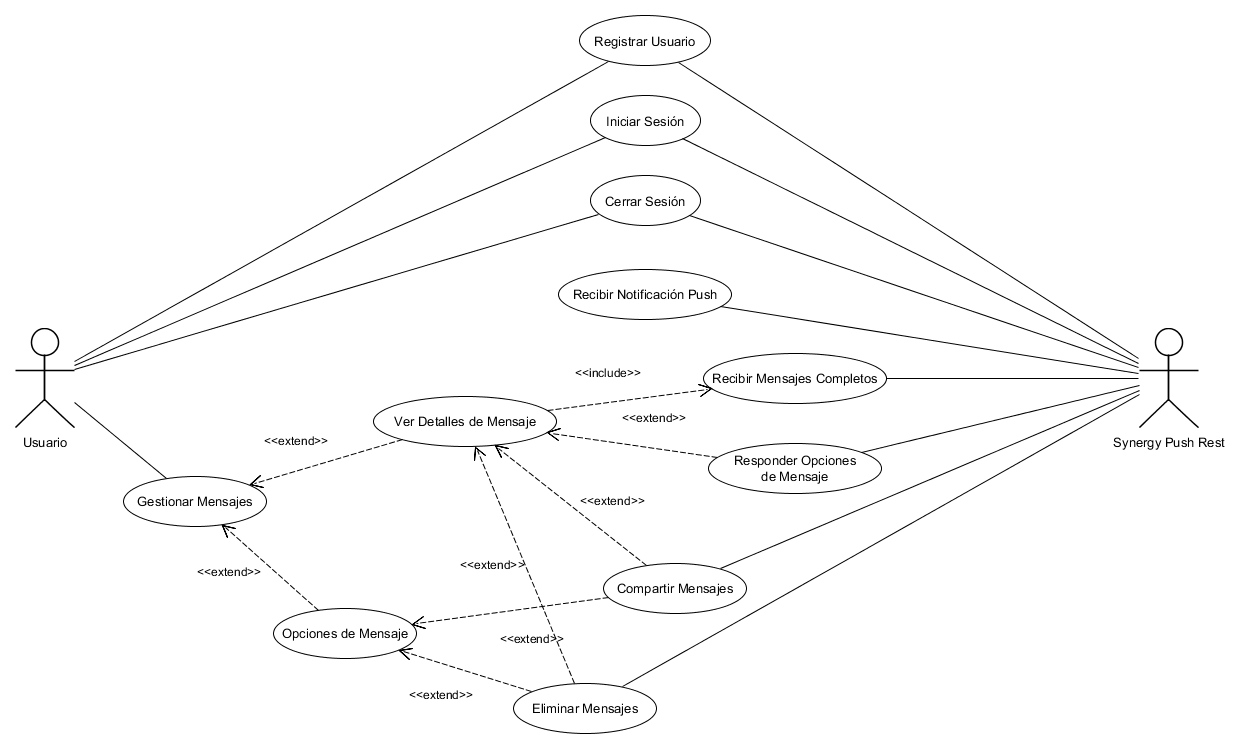
\includegraphics[scale=0.3,type=png,ext=.png,read=.png,angle=0,origin=c]{imagenes/Diagrama_de_Casos_de_Uso_v1_5}
  \caption{Diagrama de Casos de Uso inicial de Notificacones+. Elaboración propia.}
  \label{fig:dcuinicial}
\end{figure}


Luego, se estableció un plan de cuatro iteraciones de 4 semanas cada una, aproximadamente. En la primera iteración se planificó hacer todas las vistas tanto su diseño como su implementción en Ionic con HTML5/CSS3. En a segunda iteración se planificó llevar a cabo los CU relacionados con “Gestionar Mensajes”. En la tercera iteración los CU relacionados con “Recibir Notificaciones Push”, “Registrarse” y “Recibir Mensajes Completos” que son las involcradas directamente con plataforma Synergy Plus.  Finalmente, en la última iteración los CU que permitan iniciar y cerrar sesión y todos los demás detalles que falten.


\section{Diseño} \label{sect:Diseno}
En esta fase, inicialmente se estudiaron los requerimientos del dueño del producto y el API REST de Synergy Plus, para así elaborar las maquetas visuales de la aplicación siguiendo los lineamientos establecidos para el desarrollo de \textit{software} de la empresa. Luego se pasó a hacer una elaboración de las vistas basadas en las maquetas mientras éstas eran aprobadas por el dueño del producto y fuera elaborado el diseño definitivo por parte del departamento de diseño. 


\subsection{Diseño de la arquitectura}
A la hora de diseñar la arquitectura de este sistema, se tuvo en consideración las siguientes importantes características:
\smallskip
\begin{itemize}[noitemsep,nolistsep]
  \item Escalabilidad: Debe poder instanciarse de manera fácil a cualquier banco (u otro cliente que necesite un producto como Notificaciones+), de manera que el producto sea rentable con una fácil personalización de acuerdo a lo que se solicite.
  \item Modularidad: Debe ser lo más modular y de bajo acoplamiento posible para evitar inconvenientes cuando se necesiten hacer cambios a la aplicación.
  \item Flexibilidad: Debe poder cambiar incluso su funcionalidad de la manera menos traumática posible.
\end{itemize}
\bigskip

\subsubsection{Vista de Escenarios}
En la Figura ~\ref{fig:cudef} se presenta el Diagrama de Casos Uso definitivo del proyecto de pasantía Notificaciones+ para Synergy-GB. Se puede ver como en el transcurrir de las iteraciones cambió el diagrama de acuerdo a nuevos requerimientos del cliente. Lo que es más pertinente de acotar es que los Casos de Uso son iguales tanto para la aplicación móvil como la aplicación web, exceptuando "Recibir Notificaciones Push" que es exclusivo de la aplicación móvil.

\begin{figure}[H]
  \centering
  
\includegraphics[scale=0.3,type=png,ext=.png,read=.png,angle=0,origin=c]{imagenes/Diagrama_de_Casos_de_Uso_v2_0}
  \caption{Diagrama de casos de uso definitivo de Notificaciones+. Elaboración propia.}
  \label{fig:cudef}
\end{figure}


En la Figura ~\ref{fig:cupush} se presenta la especificación del CU “Recibir Notificación Push”. En el Apéndice B se pueden consultar las especificaciones de todos los CU del diagrama de la Figura ~\ref{fig:cudef}.

\begin{figure}[ht]
  \centering
  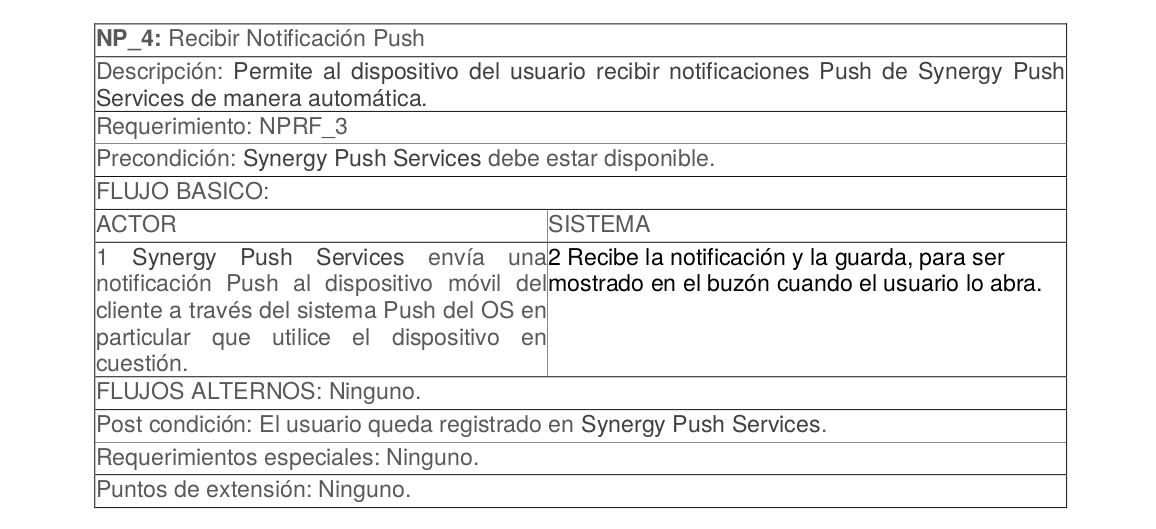
\includegraphics[scale=0.4,type=png,ext=.png,read=.png,angle=0,origin=c]{imagenes/cupush}
  \caption{Especificación del Caso de Uso “Recibir Notificación Push”. Elaboración propia.}
  \label{fig:cupush}
\end{figure}


\subsubsection{Vista Lógica}
Las aplicaciones (web y móvil) estarán conformadas por clases que se encargarán de definir los objetos que se manejan en el sistema y su relación. A continuación, en la Figura ~\ref{fig:clases} se muestra el Diagrama de Clases para Notificaciones+, el cual representa la Vista Lógica de la misma. 

\begin{figure}
  \centering
  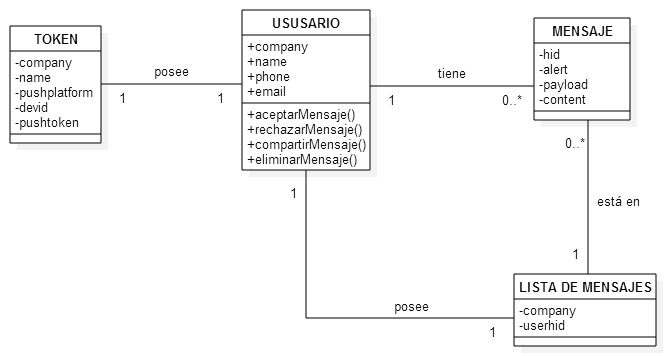
\includegraphics[scale=0.4,type=png,ext=.png,read=.png,angle=0,origin=c]{imagenes/Diagrama_de_Clases}
  \caption{Diagrama de Notificaciones+. Elaboración propia.}
  \label{fig:clases}
\end{figure}


En el diagrama de clases se pueden observar las estructuras manejadas por la plataforma Synergy Push y por lo tanto por la aplicación.


\subsubsection{Vista de Desarrollo}
La vista de desarrollo de la arquitectura de Notificaciones+ se ve reflejada en el Diagrama de Componentes que se muestra en la Figura ~\ref{fig:componentes}


\begin{figure}
  \centering
  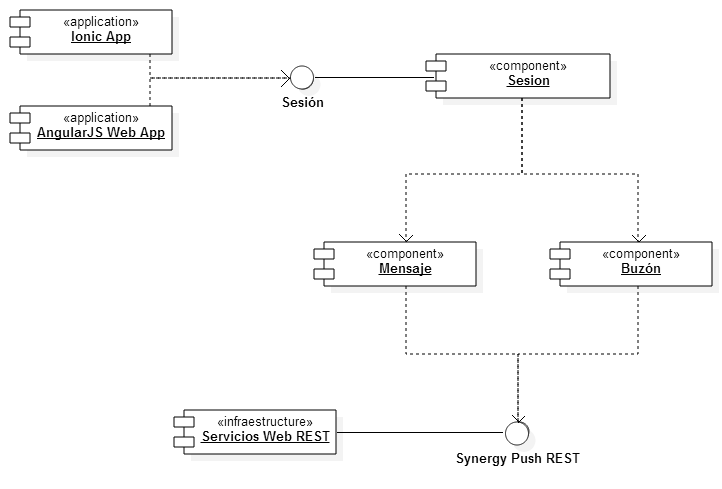
\includegraphics[scale=0.5,type=png,ext=.png,read=.png,angle=0,origin=c]{imagenes/Diagrama_de_Componentes}
  \caption{Diagrama de Componentes de Notificaciones+. Elaboración propia.}
  \label{fig:componentes}
\end{figure}


En este diagrama se puede observar el patrón de diseño MVC (Model-View-Controller) ya que cada capa representa un elemento de los anteriores, se aprecia como Ionic App y AngularJS Web App representan la capa de las vistas (View). Para el caso de la Sesión y cada uno de los siguientes dos componentes: Mensaje y Buzón, representan, en conjunto, el controlador (Controller). Y para finalizar, la capa de servicios de Notificaciones+ representa los datos o el modelo como tal (Model).


\subsubsection{Vista de Implantación}
La vista de implantación de la arquitectura de Notificaciones+ se ve reflejada en el Diagrama de Despliegue que se muestra en la Figura ~\ref{fig:despliegue}

\begin{figure}[H]
  \centering
  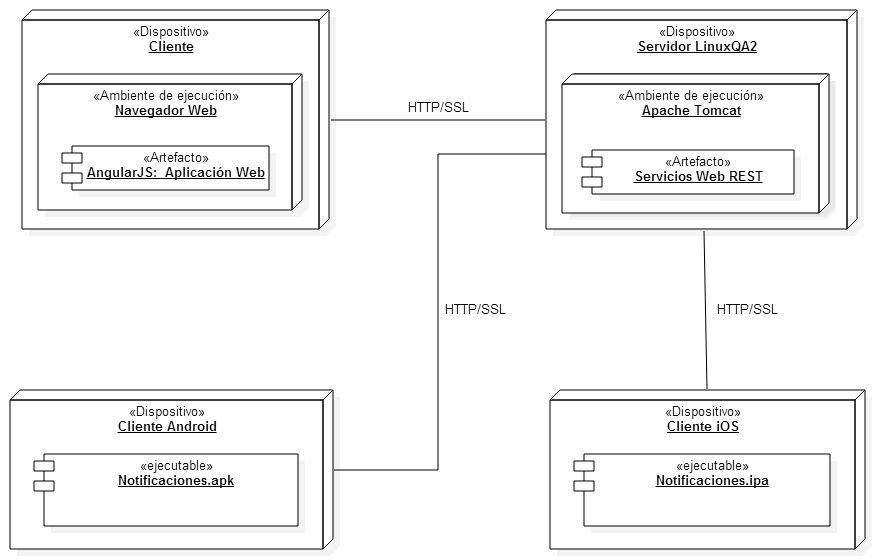
\includegraphics[scale=0.4,type=png,ext=.png,read=.png,angle=0,origin=c]{imagenes/Diagrama_de_Despliegue}
  \caption{Diagrama de Despliegue de Notificaciones+. Elaboración propia.}
  \label{fig:despliegue}
\end{figure}


Se puede ver como co-existen las aplicaciones móviles (para Android y iOS) junto con la aplicación web, e interactúan con los servicios web Rest cuando las aplicaciones se encuentran todas desplegadas.
Es importante aclarar que la comunicación se realiza a través de HTTP debido a que la plataforma Synergy Push todavía es un prototipo. Posteriormente cada una de estas se comunicará a través de HTTPS/SSL. La información que se comparte entre los nodos se encuentra en formato JSON.


\subsubsection{Vista de Procesos}
La Vista de Procesos no fue desarrollada, dado que la aplicación no resuelve aspectos de concurrencia de usuarios y de datos. Los mismos son resueltos por la arquitectura Synergy Push y el sistema bancario al que se instancie la aplicación.


\subsubsection{Vista de Datos}
La Vista de Datos no fue desarrollada dado que la aplicación como tal no cuenta con una base de datos propia. Ésta se alimenta de datos provistos por un core bancario debido al marco de trabajo de Synergy-GB. 


Es importante mencionar que cuando la aplicación sea instanciada para algún banco particular, se alimentará de los datos expuestos por dicho banco. Esos datos corresponden a los atributos de las clases del diagrama de clases mostrado en la Figura  ~\ref{fig:clases}.


\subsection{Planificación del desarrollo}
Se armó un plan inicial de desarrollo basado en los objetivos del proyecto descritos en la introducción del presente informe, lo que se planteaba en el plan de trabajo y los requerimientos que se levantaron junto con el cliente.
Este plan consta de cuatro iteraciones, de unas 4 semanas de duración cada una, aproximadamente. El mismo sufrió varios cambios a medida que se implementaban las funcionalidades para incluir actividades que no habían sido previstas, reestablecer prioridades en el desarrollo, y demás actividades que permitiesen gestionar los cambios en el proceso de construcción. En la Tabla ~\ref{table:iteraciones} se describen los objetivos de cada iteración.


\begin{table}
%\centering 
\begin{tabular}{| p{2.5cm} | p{13.5cm} |}
\hline 
\bfseries \footnotesize {Iteración} & \bfseries \footnotesize {Objetivos finales} \\ 
\hline 
\bfseries \footnotesize {Iteración 1} & 
\begin{itemize}[noitemsep,nolistsep]
  \item \footnotesize Diseño detallado e implementación del módulo de notificaciones y alertas e integración con Synergy Push:
  \begin{itemize}[noitemsep,nolistsep]
    \item \footnotesize Envío de notificaciones interactivas y recepción de respuestas
    \item \footnotesize Envío de información promocional con contenido Web
    \item \footnotesize Envío de recibos de transacciones realizadas en otros canales
  \end{itemize}
\end{itemize}
\\ \hline 
\bfseries \footnotesize {Iteración 2} & 
\begin{itemize}[noitemsep,nolistsep]
  \item \footnotesize Diseño detallado e implementación de la aplicación móvil y web de notificaciones y alertas:
  \begin{itemize}[noitemsep,nolistsep]
	   \item \footnotesize Gestión de notificaciones y respuestas
  \end{itemize}
  \item \footnotesize  Diseño detallado e implementación de la aplicación móvil en phonegap, para las funcionalidades de notificación y alertas
\end{itemize}
\\ \hline 
\bfseries \footnotesize{Iteración 3} & 
\begin{itemize}[noitemsep,nolistsep]
  \item \footnotesize Diseño detallado e implementación de la aplicación móvil en phonegap incluyendo todas sus funcionalidades. 	
\end{itemize}
\\ \hline 
\bfseries \footnotesize{Iteración 4} & 
\begin{itemize}[noitemsep,nolistsep]
  \item \footnotesize Prueba de la aplicación móvil en las distintas plataformas móviles, y desarrollo de ajustes para problemas específicos de plataformas.
  \item \footnotesize Finalización de los casos pendientes de las iteraciones anteriores.  
\end{itemize}
\\ \hline 
\end{tabular}
\footnotesize \caption{Iteraciones de desarrollo de Notificaciones+ y sus objetivos. Elaboración Propia.}
\label{table:iteraciones}
\end{table}


\section{Construcción} \label{sect:Construccion}
Esta fase se centró en el desarrollo de las funcionalidades y Casos de Uso previamente definidos, siguiendo la planificación especificada en la Tabla ~\ref{table:iteraciones}. La misma se llevó a cabo de acuerdo a los estándares de Synergy-GB promoviendo la modularidad, reutilización y gerencia de cambio (cambios de requisitos de \textit{software} no planificados).


Al finalizar cada iteración, los componentes desarrollados fueron probados para permitir la verificación de la correctitud de las funcionalidades implementadas. Al finalizar esta etapa, dichos componentes quedaron listos para pasar a las pruebas de sistemas y de aceptación, las cuales, sobre la base de la metodología que se está utilizando (Metodología de Proyectos de Synergy-GB), se hacen en la fase de transición.


\subsection{Iteración 1}
En esta iteración se realizaron las tareas de los Sprint 1, 2, 3 y 4 (pueden consultarse a detalle en el Apéndice C). Para cumplir los objetivos propuestos para esta etapa, en primer lugar, se realizó un estudio del API de la plataforma Synergy Push y de los requerimientos detallados del dueño del producto para realizar un diseño preliminar de la aplicación móvil, incluyendo las vistas. De la plataforma Synergy Push se dio a entender 2 distinciones esenciales del funcionamiento de la aplicación y de qué es lo que va a recibir y manejar:
\smallskip
\begin{itemize}[noitemsep,nolistsep]
  \item Notificaciones que alertan al usuario que posee un mensaje. Una notificación posee toda la información del mensaje excepto su contenido. El usuario puede recibir notoficaciones de dos maneras distintas:
  \begin{itemize}[noitemsep,nolistsep]
    \item Vía Push: exclusivo para dispositivos móviles. Son recibidos siempre y cuando el usuario haya hecho login, aún así el dispositivo esté en descanso y bloqueado.
    \item Vía HTTP: se reciben dentro de la aplicación, tanto móvil como web, a solicitud del usuario. Siempre se puede recibir la notificación de un mensaje mientras éste no haya sido abierto.
  \end{itemize}
  \item Mensajes: versión completa de la notificación, que posee un contenido de texto o dirección web. Una vez abierto se elimina de la plataforma Synergy Push y quedará contenido en el dispositivo móvil o en el navegador dónde el usuario lo haya abierto con la aplicación web.
\end{itemize}
\bigskip


En segundo lugar, una vez entregada una versión inicial de los diseños de vistas y funcionalidades, se procedió a empezar a implementar las vistas preliminares a la espera de las vistas oficiales del departamento de diseño. Una vez hechas las vistas preliminares se pasó a implementar las funcionalidades básicas de transición.


Al ser recibido el diseño de la aplicación del departamento de diseño de la empresa se pasó a adaptar las vistas ya hechas. Las vistas no eran convencionales y no se podían hacer con las utilidades que trae Ionic por defecto, así que se tuvo que hacer mucha investigación y experimentación para manipular el código CSS para lograr lo exigido.


Luego, se empezó la integración de lo ya programado a la plataforma Android y así empezar a implementar la recepción de las notificaciones Push, fundamentales para esta aplicación. Debido a la naturaleza experimental de esta funcionalidad, nueva en el framework Ionic, requirió gran cantidad de tiempo y pruebas, exclusivamente en Android; la creación de la versión móvil iOS se dejó para después de que la versión Android tuviera todas sus funcionalidades fundamentales implementadas, a petición del líder de movilidad de la empresa encargado de supervisar el proyecto.


Al finalizar esta iteración se hicieron pruebas manuales por parte del desarrollador usando directamente la plataforma Synergy Push para probar la recepción y el manejo de las notificaciones Push. Haciendo esto se descubrieron varios de los errores superados en la sección de Retos y Logros.


\subsection{Iteración 2}
En esta iteración se realizaron las tareas de los Sprint 5 y 6 (pueden consultarse a detalle en el Apéndice C), que incluyen las funcionalidades: login, apertura y recepción de mensajes, eliminar mensajes, registro y modificar perfil. Se tuvo que hacer también las vistas de registro y modificar perfil ya que no habían sido tomadas en consideración por el departamento de diseño ni el dueño del producto, para esto fue necesario que el desarrollador y el líder de departamento de diseño las hicieran en conjunto.


En esta iteración estaba planificado la implementación del grueso de las funcionalidades de la aplicación móvil multiplataforma y el comienzo de la aplicación web, con la intención de empezar la aplicación web desde cero, pero después de hecha la estructura principal se tomó la decisión de usar una plantilla web propiedad de la empresa, que no estaba lista todavía, así que todo lo que era desarrollo web fue postergado para la última iteración.


La aplicación está diseñada para trabajar en conjunto con la plataforma Synergy Push y con algún sistema del cliente que compre la aplicación, y como dicho sistema no existe todavía hay algunas cosas que tuvieron que resolverse:
\smallskip
\begin{itemize}[noitemsep,nolistsep]
  \item La aplicación debe iniciar sesión con la página del cliente (un banco u otro) así que se creo un mini servidor que aceptara inicio de sesión con el específico único de implementar esta funcionalidad.
  \item La aplicación debe registarse con Synergy Push y el sistema del cliente al mismo tiempo así que se hizo uso nuevamente del mini servidor provisional para que aceptara registro de la aplicación tanto web como móvil.
  \item Los mensajes deberían ser enviados por el sistema del cliente a la plataforma Synergy Push y es ésta la que lo gestiona y envía a la aplicación de los usuarios particulares. Para implementar y hacer pruebas de esto simplemente se hizo uso del modo desarrollador de Synergy Push y se enviaron los mensajes manualmente.
  \item Las respuestas de los mensajes interactivos son recibidas por el mismo sistema del cliente que envió dichos mensajes en primer lugar, para eso nuevamente se hizo uso del mini servidor provisional que recibiera las respuestas.
\end{itemize}
\bigskip


Luego se pasó a agregar guardado de mensajes persistente en la aplicación móvil, de manera que los mensajes abiertos no se perdieran hasta que el usuario los borrara.


Luego se exportó todo lo hecho tanto a la plataforma Android como a la plataforma iOS, descubriendo el error de Synergy Push para enviar notificaciones Push para iOS. La habilidad de recibir notificaciones Push por parte de la aplicación móvil fue comprobada por el desarrollador por medio de otros programas auxiliares. Todas las demás funcionalidades implementadas funcionan en ambas plataformas.


Al finalizar la iteración, se realizaron pruebas unitarias para todas las funcionalidades implementadas. Al igual que en la iteración anterior, estas pruebas fueron llevadas a cabo de forma manual utilizando la plaraforma Synergy Push y el mini servidor provisional.


\subsection{Iteración 3}
En esta iteración se realizaron las tareas de los Sprint 7 y 8 (pueden consultarse a detalle en el Apéndice C) que incluyen las funcionalidades: \textit{pull refresh}, autenticación, compartir mensajes y botones de respuesta, además del arreglo de un bug de la recepción Push para Android detectado por el desarrollador. Esta iteración consiste básicamente en terminar los últimos detalles y resolver los errores de la aplicación móvil.


Primero se implementó la funcionalidad \textit{pull refresh}, que simplemente consiste en darle poder al usuario para hacer que la aplicación buscara notificaciones nuevas desde el buzón vía HTTP sin tener que esperar que llegara la notificación vía Push. Se tuvo que hacer uso de un algoritmo muy eficiente para mezclar la lista de notificaciones entrante con la que ya estaba almacenada en el teléfono para ahorrar recursos computacionales del dispositivo. Este algoritmo consiste en una mezcla de listas de JavaScript usando la función "map()".

Luego se hizo la funcionalidad autenticar, que simplemente consistió en una mejora del login ya implementado. Se hizo que la aplicación mandara una solicitud en particular al mini servidor y que este devolviera a su vez una respuesta particular que le permitiera a la aplicación avanzar a la siguiente vista.


Para la funcionalidad de compartir solo se hizo uso del plugin de Cordova diseñado para eso, que funciona adecuadamente para ambas plataformas móviles y comparte los mensajes de Notificaciones+ a través de cualquier aplicación de mensajería o de red social que el usuario tenga instalada en su dispositivo. 


Los botones de respuesta se implementaron haciendo uso del mini servidor provisional para que recibiera dichas respuestas. Se tuvo una reunión con el dueño del producto y este indicó que los mensajes se podían responder solamente una vez y así fue implementado.


La última tarea del Sprint consistía en resolver un error de recepción Push en la versión Android de Notificaciones+, dónde las notificaciones Push no son recibidas por la aplicación si esta estaba en segundo plano. Se hizo investigación y varias pruebas hasta localizar el error en el código fuente del plugin de recepción Push. Para resolver esto se tuvo que modificar dicho código fuente para adaptarlo a las necesidades de la aplicación. Se desconoce si este error se presenta también para iOS ya que como se ha mencionado antes, la plataforma Synergy Push no es capaz de mandar notificaciones Push a iOS todavía.


\subsection{Iteración 4}
En esta iteración se realizaron las tareas de los Sprint 9, 10 y 11 (pueden consultarse a detalle en el Apéndice C) que abarca todo el desarrollo de la aplicación Notificaciones+ Web. Una vez obtenido acceso a la plantilla web de la empresa, se pasó a adaptar las partes útiles las necesidades de la aplicación tanto visual como en funcionalidad. Debido a que no era necesario hacer una vista desde cero sino adaptar una, los aspectos visuales fueron sugeridos directamente por el líder del departamento de diseño sin necesidad de realizar un diseño completo.


Primero se adaptó una vista de manejador de correo electrónico perteneciente a la plantilla para hacer de vista buzón de Notificaciones+. Luego se pasó a hacer las funcionalidades. Después de toda la experiencia adquirida en el desarrollo de la aplicación en Ionic, el desarrollo web fue relativamente sencillo. Una vez completadas todas las funcionalidades de la vista buzón, incluyendo filtro por tipo de mensajes y por texto introducido por el usuario, se pasó a desarrollar las siguientes vistas.


Las vistas y funcionalidades de login, registro y modificar perfil se adaptaron igualmente de las páginas prediseñadas de la plantilla. La pantalla de modificar perfil fue una adaptación de la de registro ya que no existía un equivalente en la plantilla. Sus funcionamientos fueron análogos a la versión móvil de Ionic, haciendo uso de las mismas técnicas de programación y del mini servidor provisional.


El último requisito que se atacó fue la vista de detalles de mensajes, y sus funcionalidades inherentes como compartir, eliminar y responder mensajes. La respuesta de mensajes es análoga a la de la aplicación móvil. La funcionalidad de eliminar mensajes no lo fue tanto ya que en la aplicación web se puede enviar los mensajes a una papelera desde el buzón antes de ser borrados y luego en la papelera se pueden eliminar varios o todos los mensajes al mismo tiempo seleccionándolos antes. Desde la vista de detalles de mensaje también se pueden borrar los mensajes pero solo definitivamente sin pasar por la papelera primero. La funcionalidad compartir requirío aplicar links directos a las redes sociales correspondientes excepto para Facebook, cuyas políticas de desarrollo obligan a registrar la aplicación Notificaciones+ para poder compartir algo.


Finalmente se hicieron pruebas manuales para verificar el correcto desempeño de todas las funcionalidades implementadas. 


\subsection{Descripción general del producto}
Al finalizar la fase de construcción, se cuenta con un prototipo funcional estable de Notificaciones+ tanto web como móvil, validado por el cliente. La aplicación permite: iniciar y cerrar sesión; recibir mensajes vía push o Internet, guardar los mensajes, compartir y eliminar mensajes.

Al abrir las aplicaciones, se muestra la pantalla de inicio de sesión, en la cual deben escribirse los datos del usuario para poder iniciar su sesión y entrar a su buzón. En la Figura ~\ref{fig:login} se muestra las capturas de pantalla de dicha vista (tanto para móvil como para web).

%%En la Figura ~\ref{fig:login} se muestra la pantalla de la página de inicio de sesión del sistema.
\begin{figure}[htp]
  \centering
  %%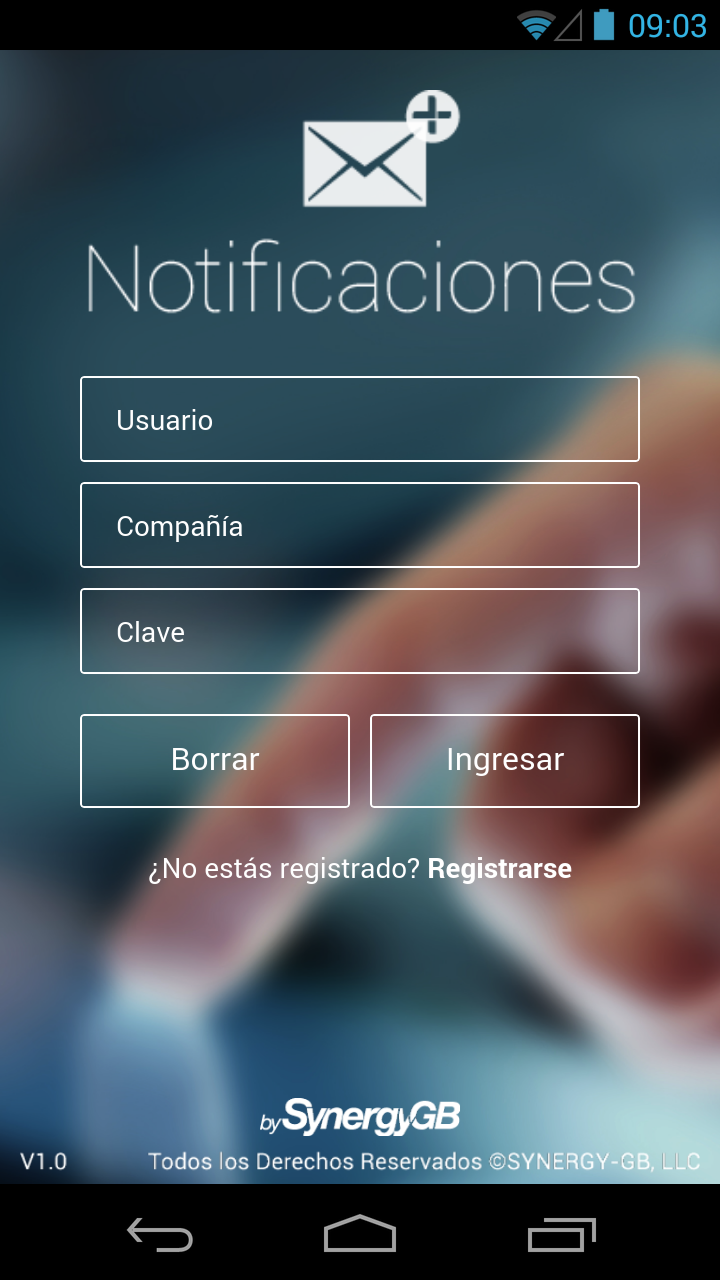
\includegraphics[width=3cm,type=png,ext=.png,read=.png,angle=0,origin=c]{imagenes/pantalla1}
  \subfloat[Versión Web]{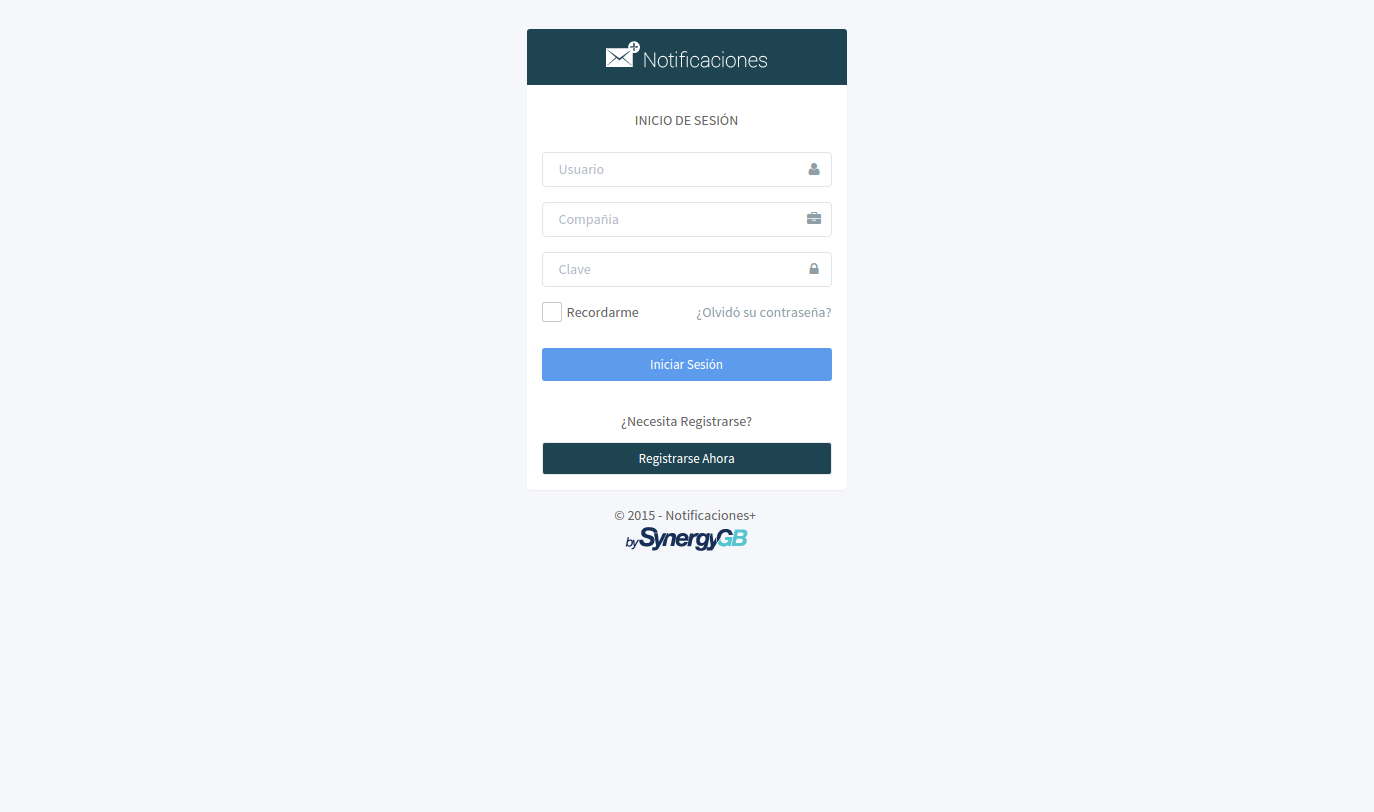
\includegraphics[width=11cm]{imagenes/Login_Web2}}
  \quad
  \subfloat[Versión Móvil]{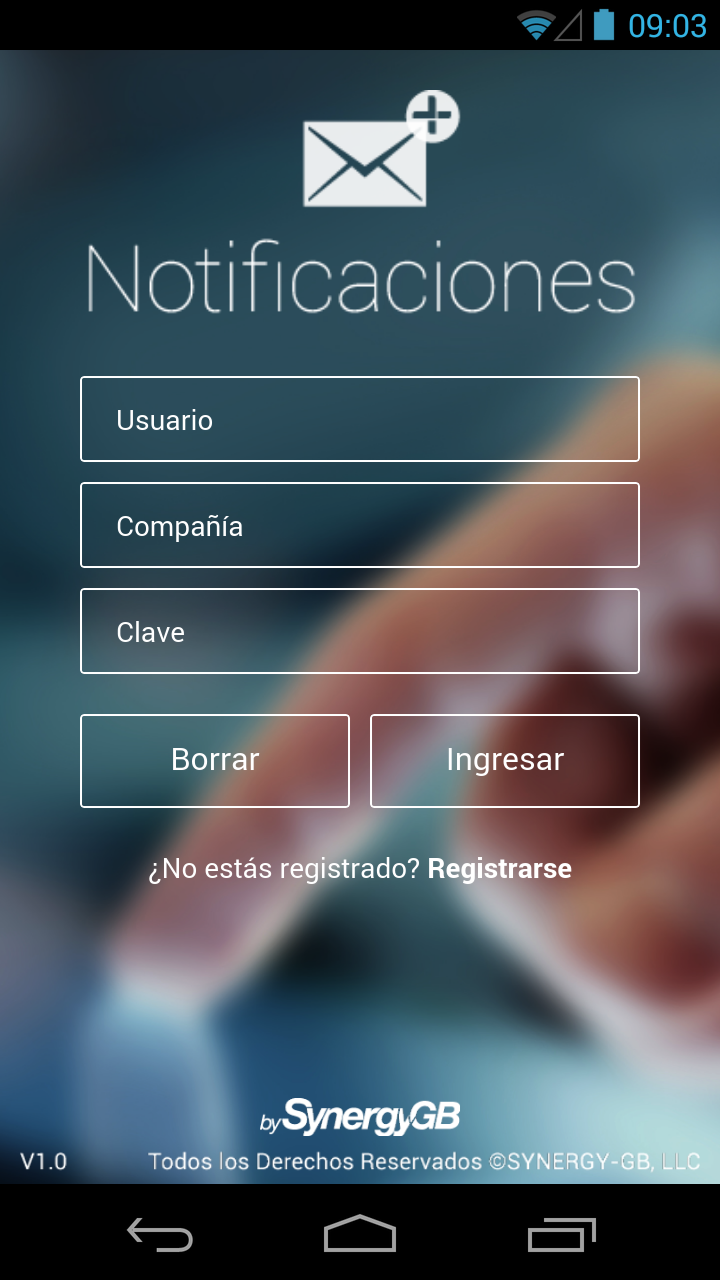
\includegraphics[width=3.5cm]{imagenes/pantalla1}}
  \caption{Pantallas de Inicio de Sesión de Notificaciones. Elaboración propia.}\label{fig:login}
\end{figure} 

Si el usuario no estrá registrado, se le da la opción al usuario de registrarse a la plataforma en la pantalla login. En la Figura ~\ref{fig:registro} se muestra la captura de pantalla de esta página.
\begin{figure}[htp]
  \centering
  %%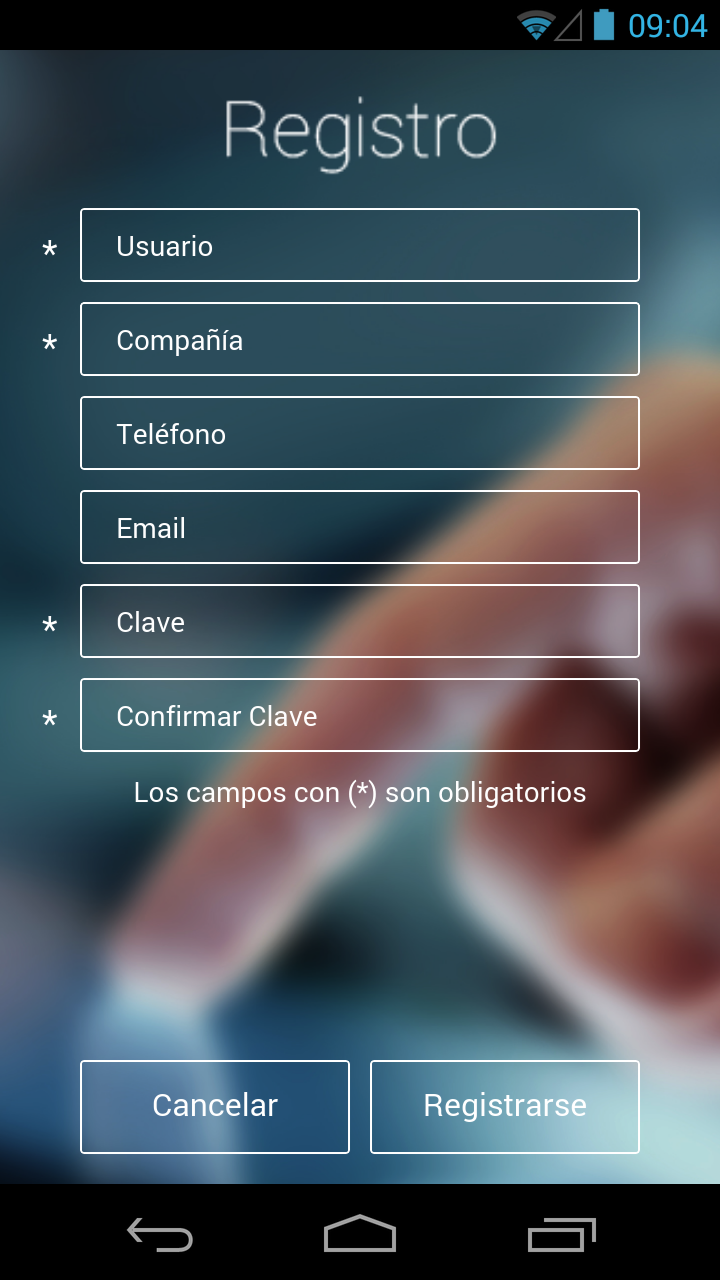
\includegraphics[width=3cm,type=png,ext=.png,read=.png,angle=0,origin=c]{imagenes/pantalla2}
  \subfloat[Versión Web]{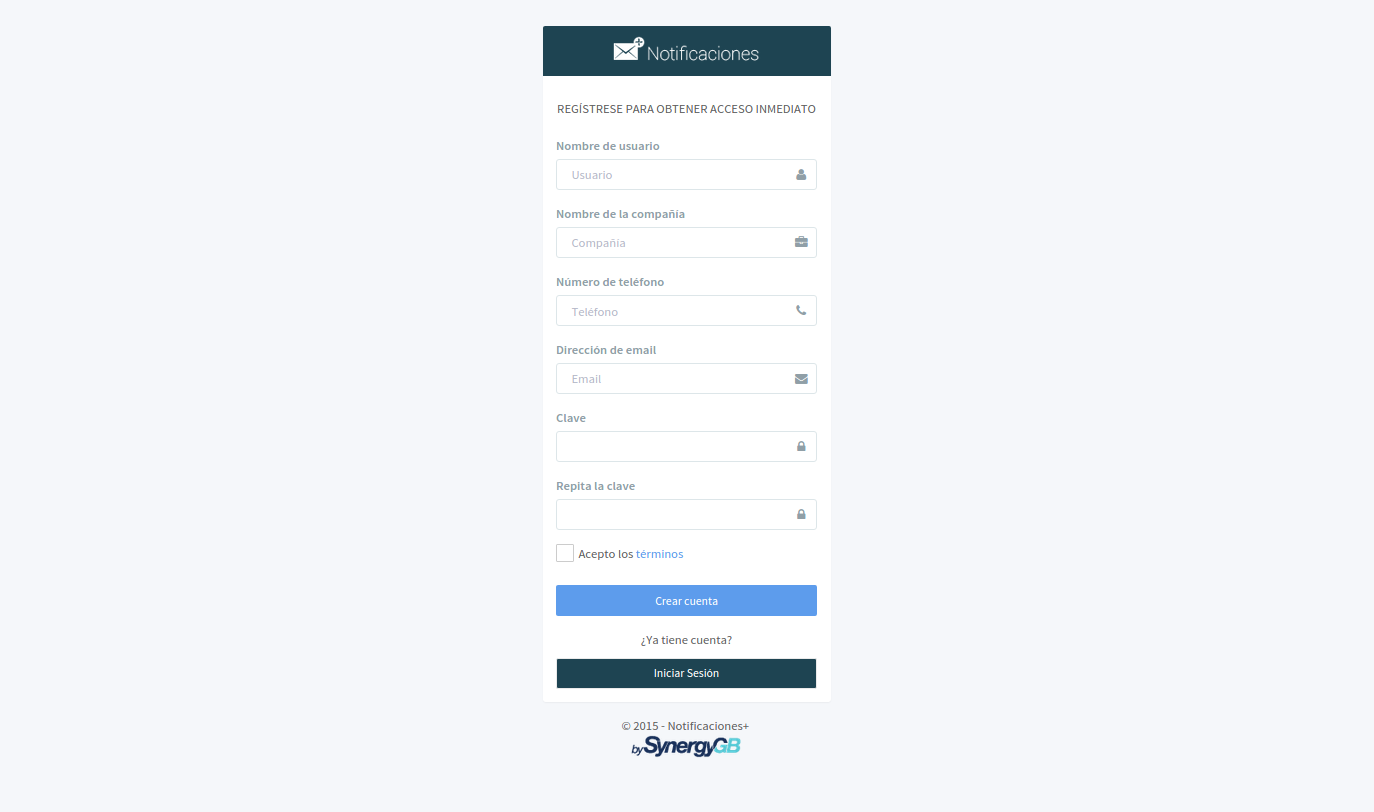
\includegraphics[width=11cm]{imagenes/Registro_Web2}}
  \quad
  \subfloat[Versión Móvil]{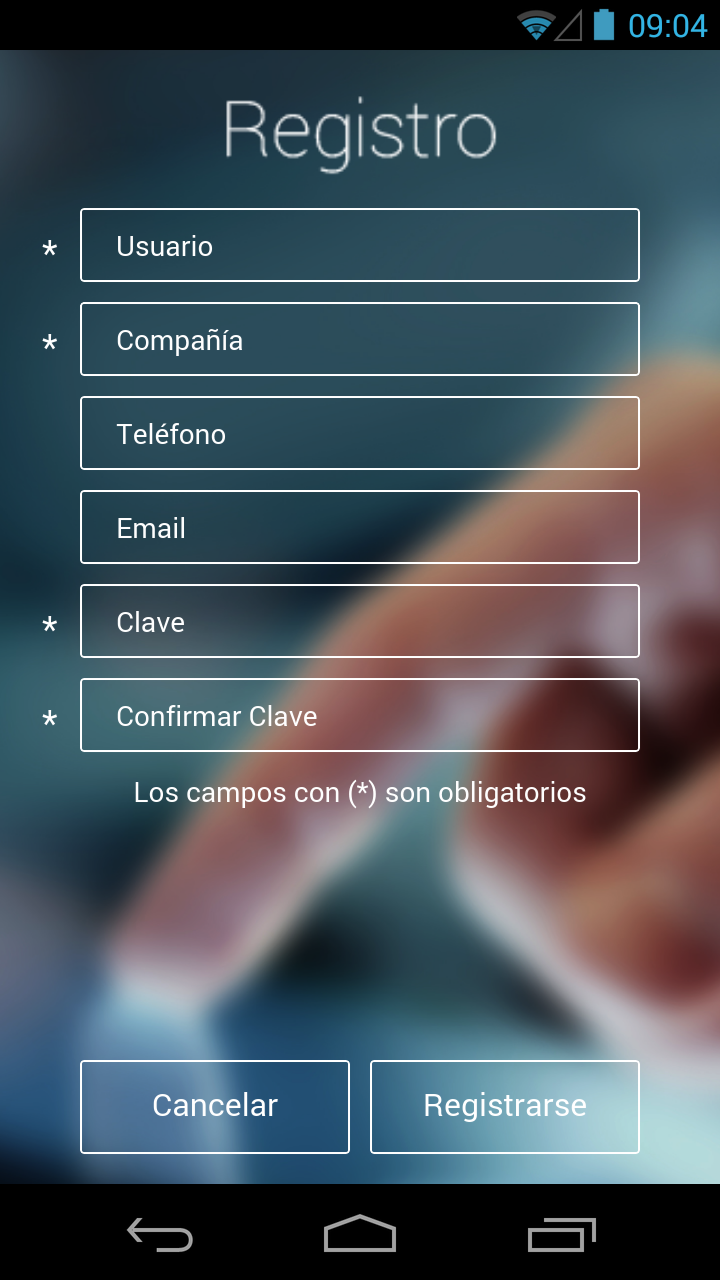
\includegraphics[width=3.5cm]{imagenes/pantalla2}}
  \caption{Pantalla de Registro. Elaboración propia.}\label{fig:registro}
\end{figure} 

Una vez iniciada la sesión del usuario se visualiza el menú principal, donde el usuario puede acceder directamente al buzón con o sin un filtro de mensajes seleccionado. Además, se le ofrece la opción de modificar su perfil. En la Figura ~\ref{fig:MenuPrincipal} se muestra la captura de pantalla de esta página.
\begin{figure}[htp]
  \centering
  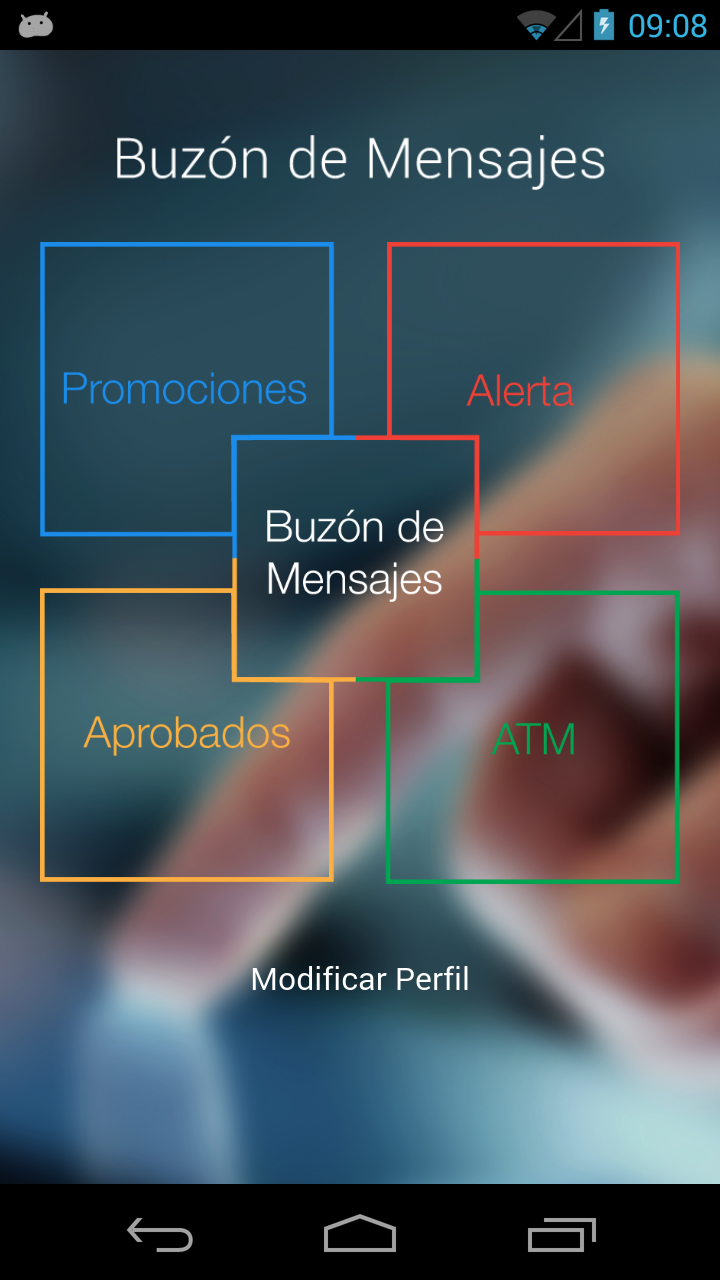
\includegraphics[width=3cm,type=png,ext=.png,read=.png,angle=0,origin=c]{imagenes/pantalla3}
  \caption{Pantalla de Menú Principal. Elaboración propia.}
  \label{fig:MenuPrincipal}
\end{figure} 

Si el usuario selecciona la opción de modificar su perfil se le muestra dicha pantalla, con el campo nombre en gris indicando que es lo único que no puede modificar. En la Figura ~\ref{fig:ModificarPerfil} se muestra la captura de pantalla de esta página, se puede acceder desde el Menú Principal en la aplicación móvil o desde el Buzón en la versión web.
\begin{figure}[htp]
  \centering
  %%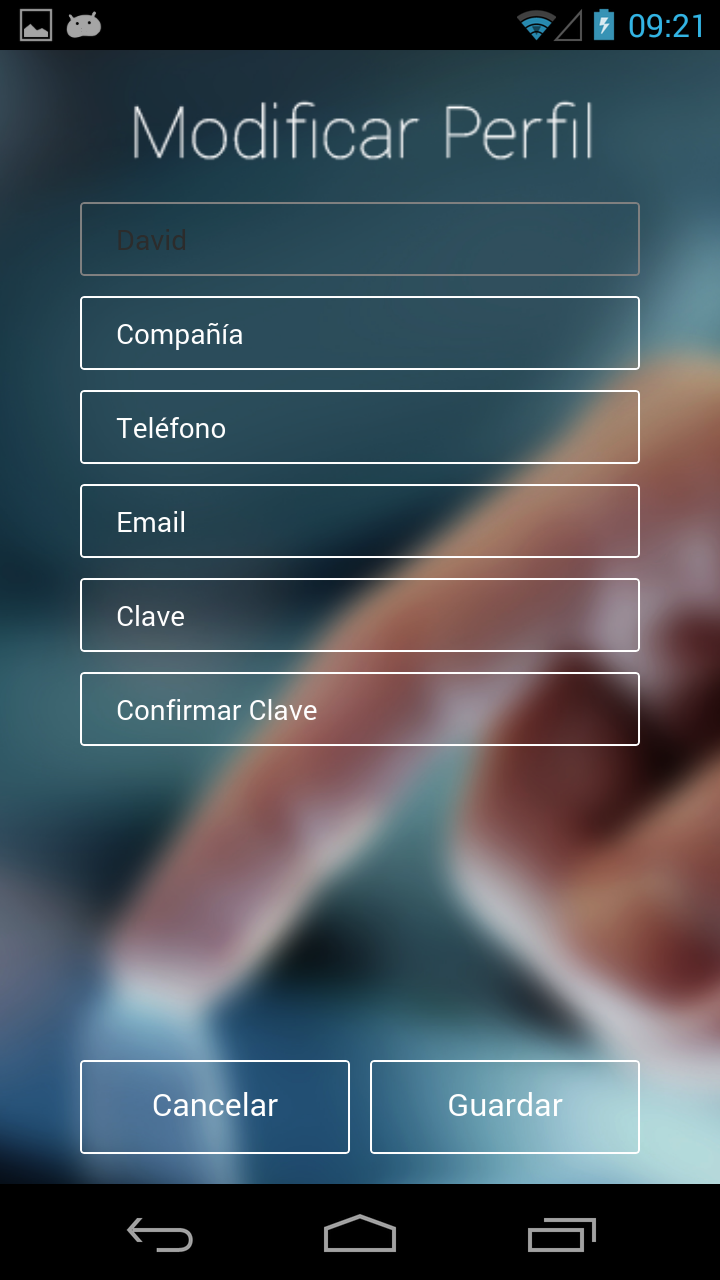
\includegraphics[width=3cm,type=png,ext=.png,read=.png,angle=0,origin=c]{imagenes/pantalla4}
  \subfloat[Versión Web]{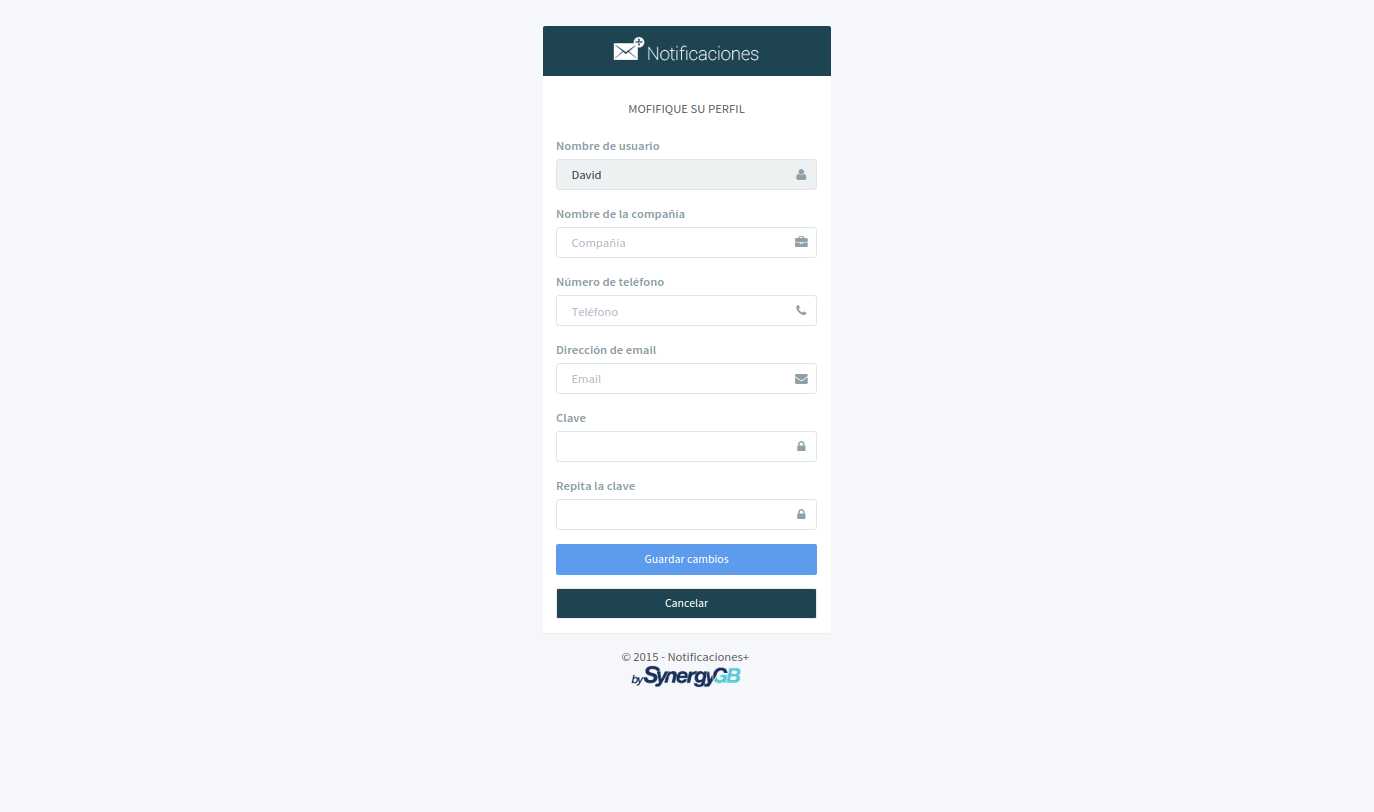
\includegraphics[width=11cm]{imagenes/Modificar_Perfil_Web2}}
  \quad
  \subfloat[Versión Móvil]{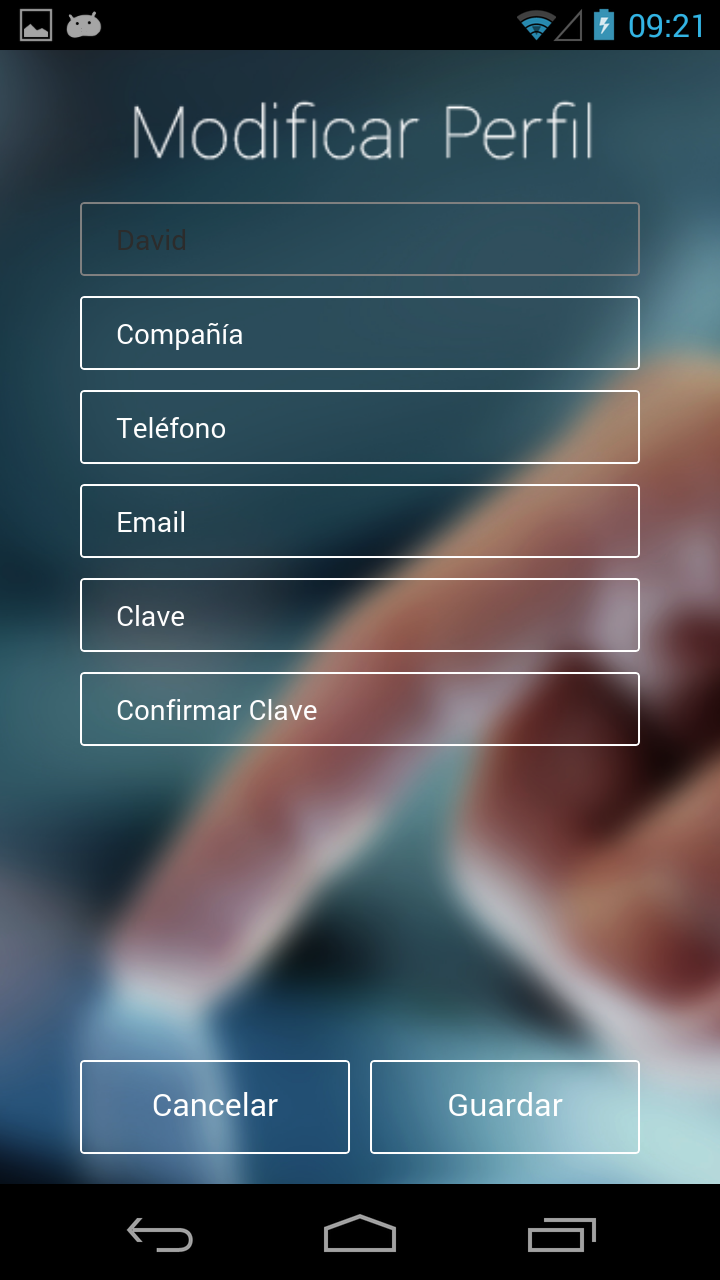
\includegraphics[width=3.5cm]{imagenes/pantalla4}}
  \caption{Pantalla Modificar Perfil. Elaboración propia.}
  \label{fig:ModificarPerfil}
\end{figure} 	

En la pantalla buzón, se muestran todos los mensajes recibidos, los cuales pueden ser filtrados por tipo al presionar uno de los botones mostrados, o por el texto que contienen en el cuadro de búsqueda. En la Figura ~\ref{fig:pantallaMulti} se puede observar la pantalla de la versión móvil sin alterar y bajo la acción de los botones. En la Figura ~\ref{fig:pantallaMultiWeb} se puede observar la pantalla de la versión web sin alterar y bajo la acción de los botones. Cabe acotar que para que aparezca el cuadro de búsqueda en la versión web hay que solicitarlo mediante el botón indicado.
\begin{figure}[htp]
\centering
  \subfloat[Buzón de mensajes]{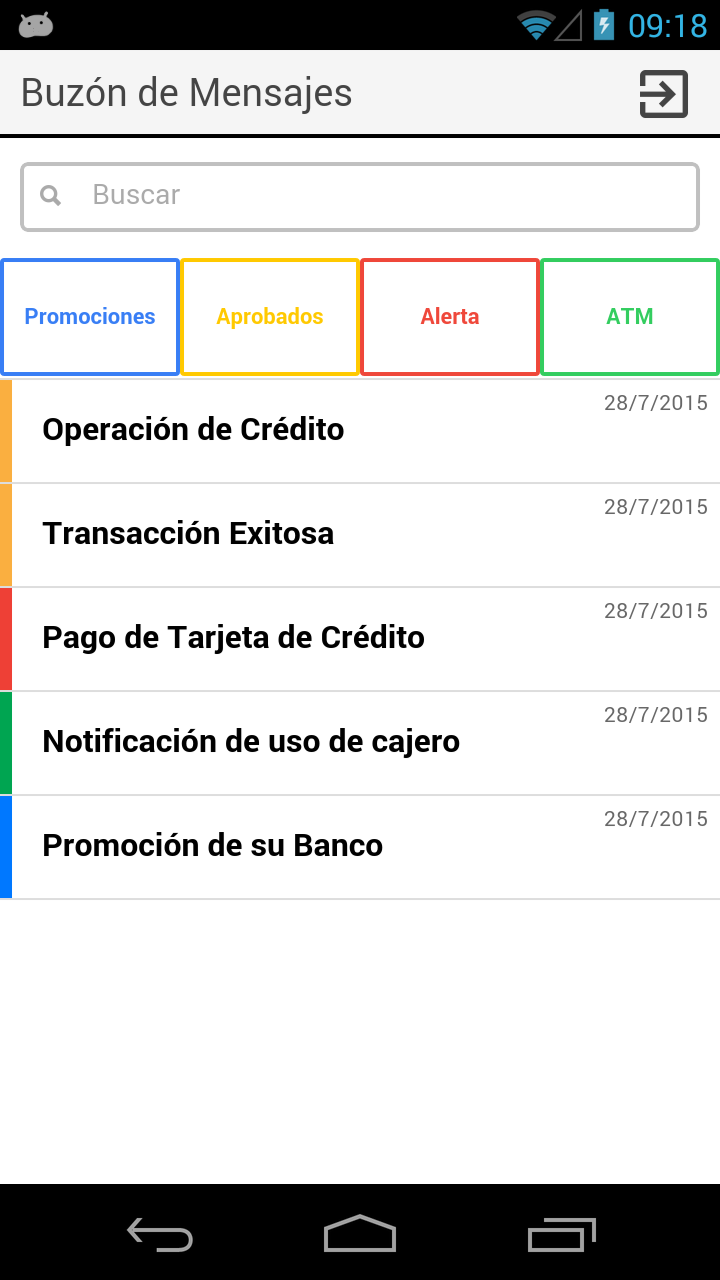
\includegraphics[width=3.5cm]{imagenes/pantalla5}}
  \quad
  \subfloat[Filtro Aprobados]{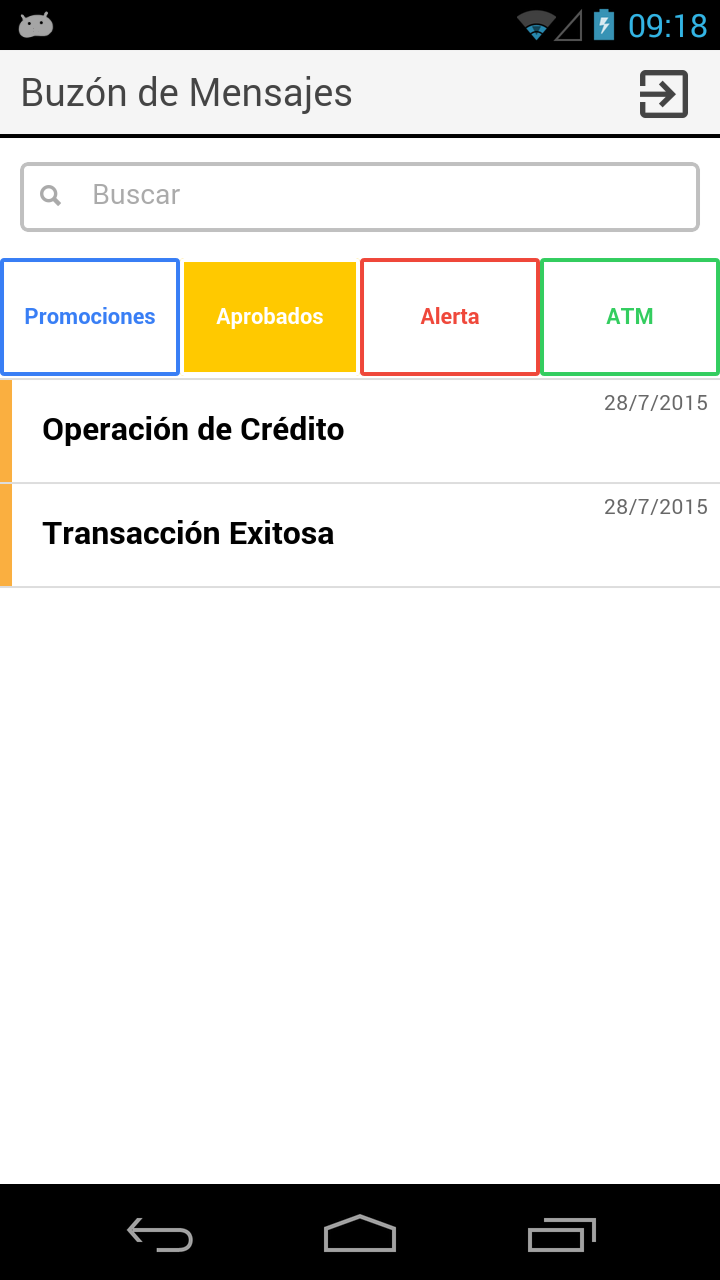
\includegraphics[width=3.5cm]{imagenes/pantalla6}}
  \quad
  \subfloat[Filtro Promociones]{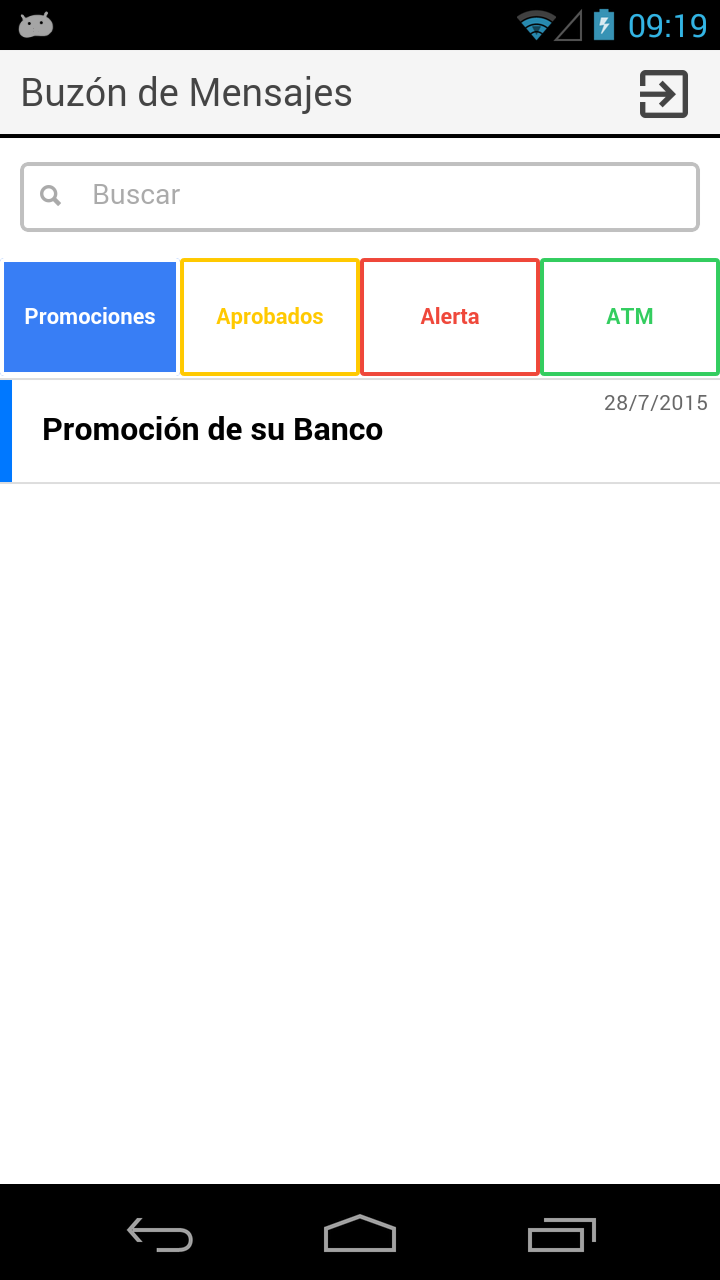
\includegraphics[width=3.5cm]{imagenes/pantalla7}}
  \quad
  \subfloat[Filtro Alerta]{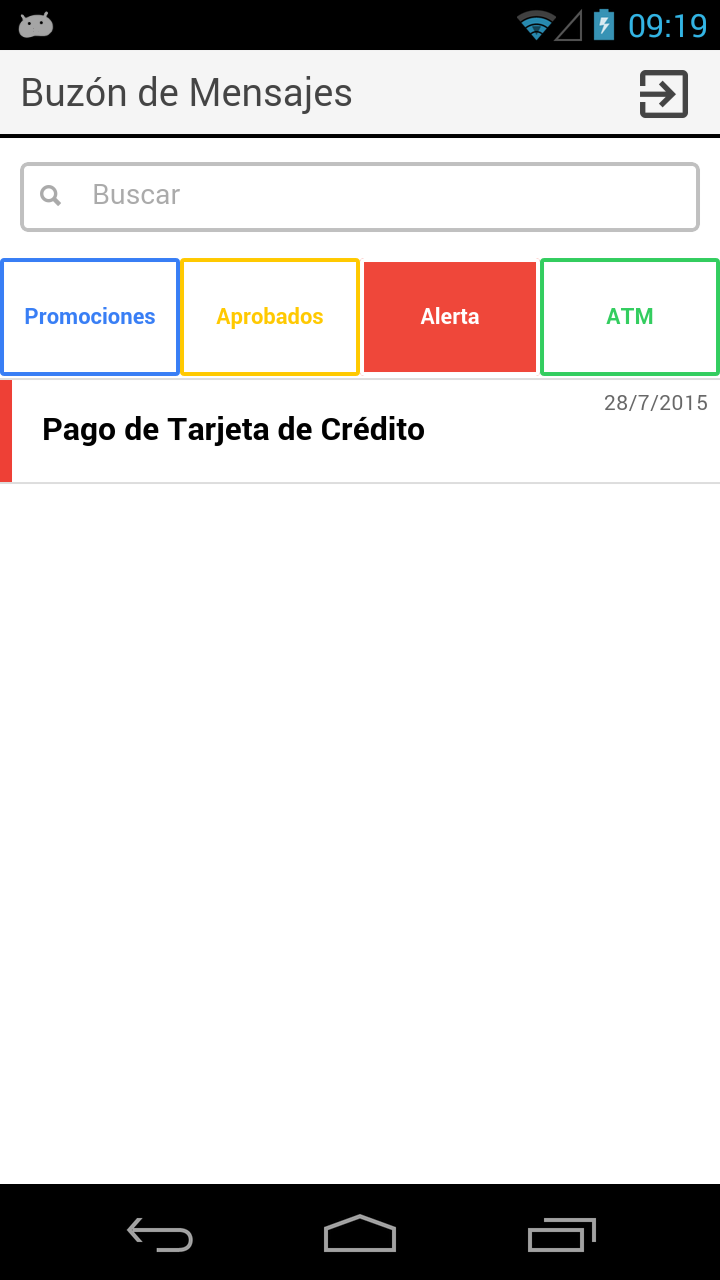
\includegraphics[width=3.5cm]{imagenes/pantalla8}}
  \quad
  \subfloat[Filtro ATM]{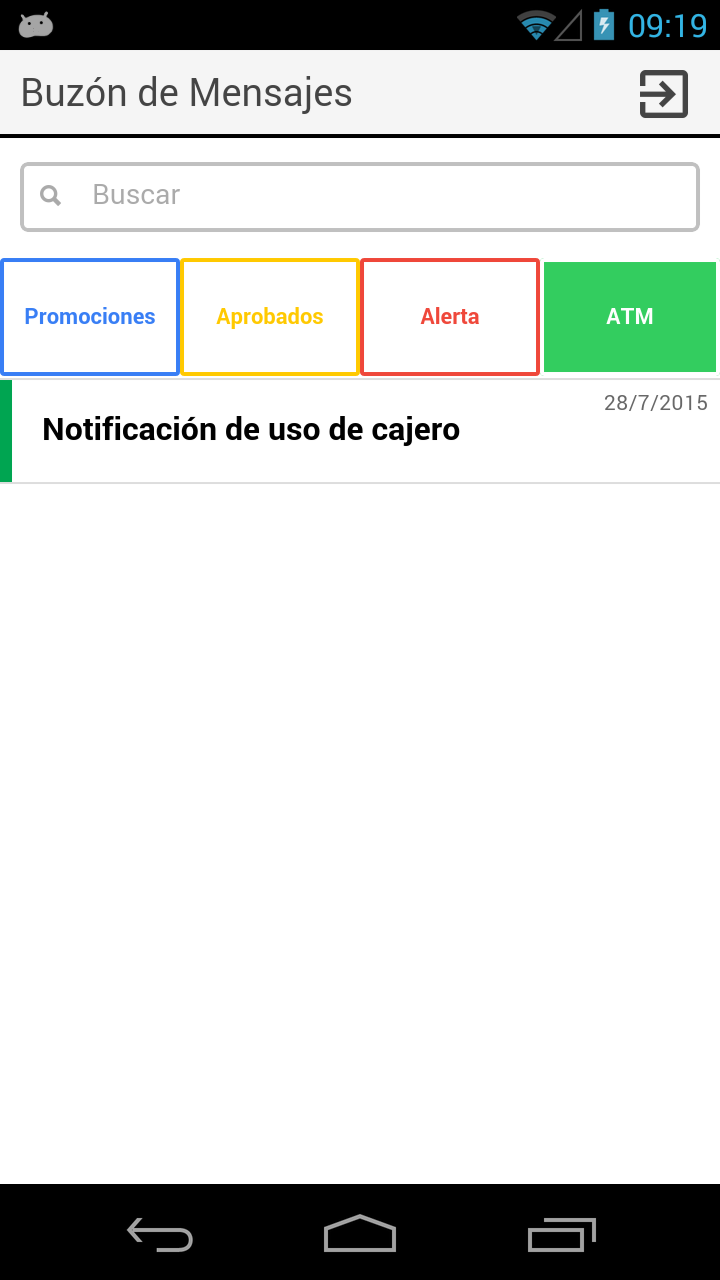
\includegraphics[width=3.5cm]{imagenes/pantalla9}} 
  \quad
  \subfloat[Mensaje leído]{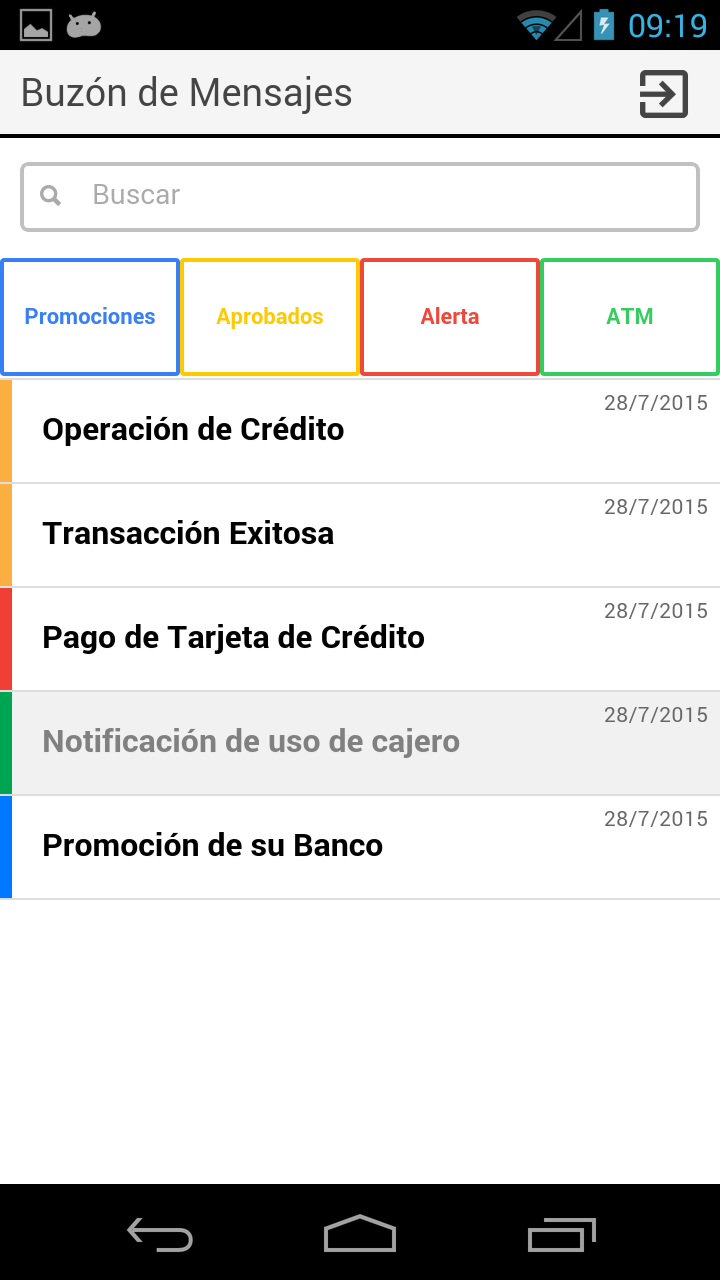
\includegraphics[width=3.5cm]{imagenes/pantalla10}}
\caption{Pantalla de Buzón con botones de filtrado versión Móvil. Elaboración propia.}\label{fig:pantallaMulti}
\end{figure}

\begin{figure}[htp]
\centering
  \subfloat[Buzón de mensajes]{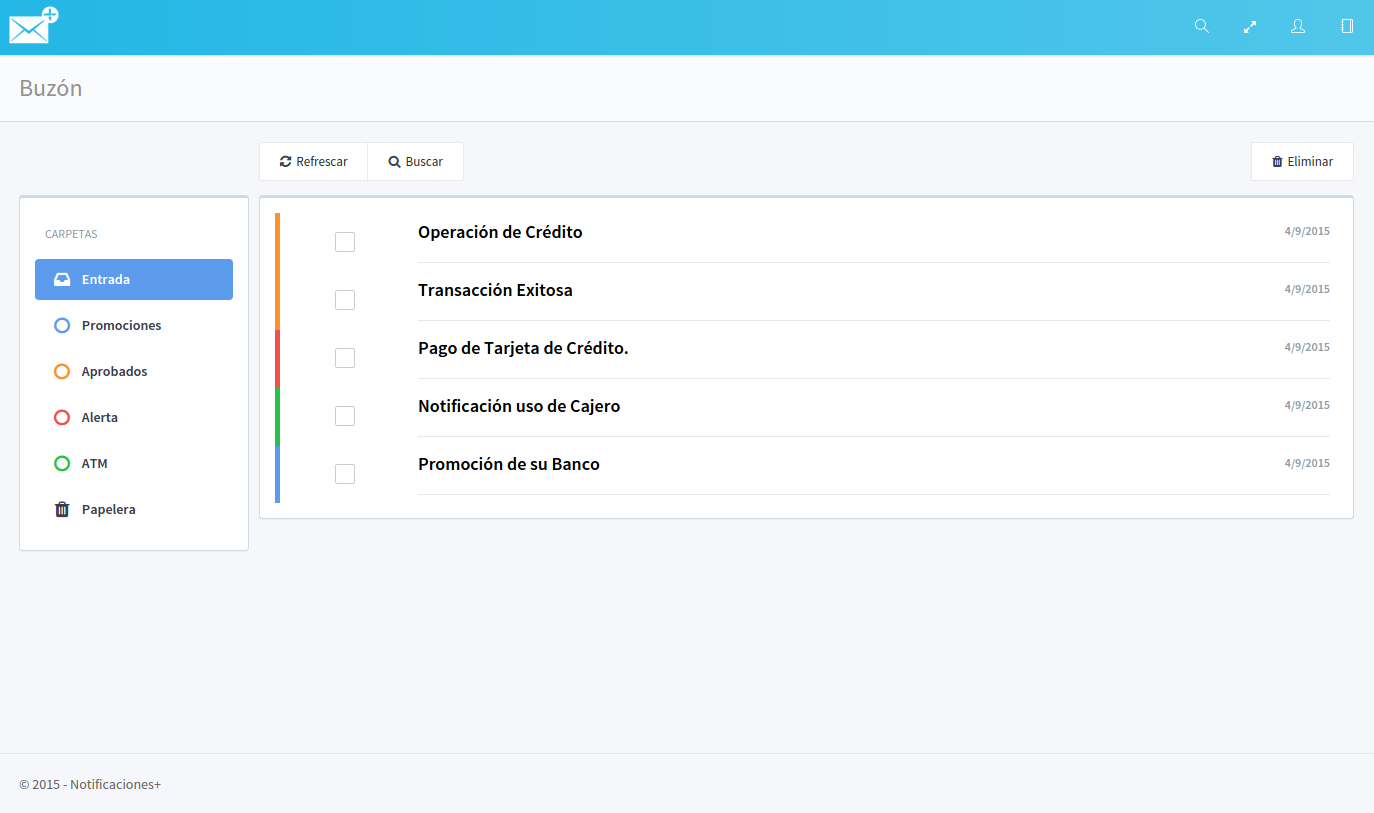
\includegraphics[width=11cm]{imagenes/Buzon_Web}}
  \quad
  % \subfloat[Filtro Aprobados]{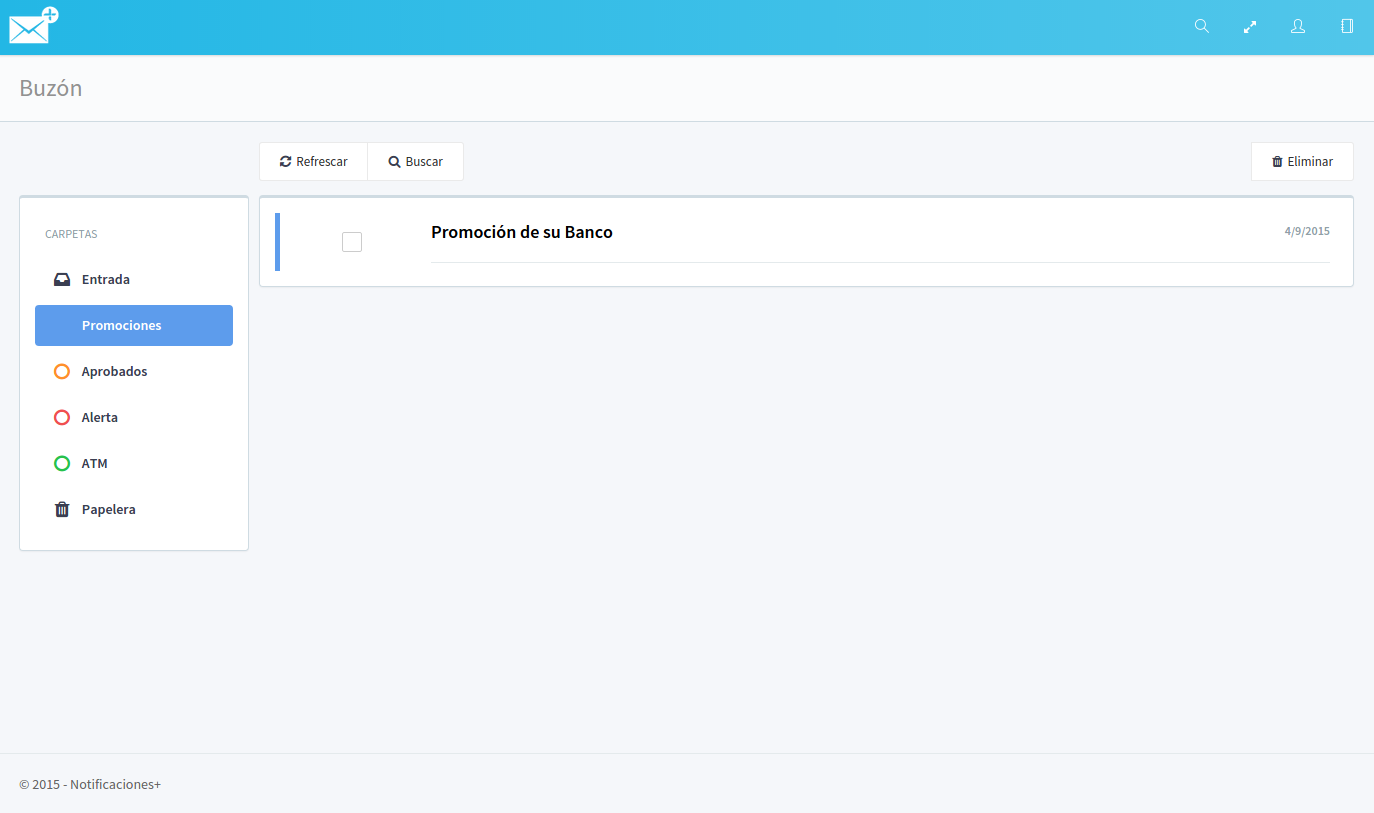
\includegraphics[width=11cm]{imagenes/Filtro1}}
  % \quad
  % \subfloat[Filtro Promociones]{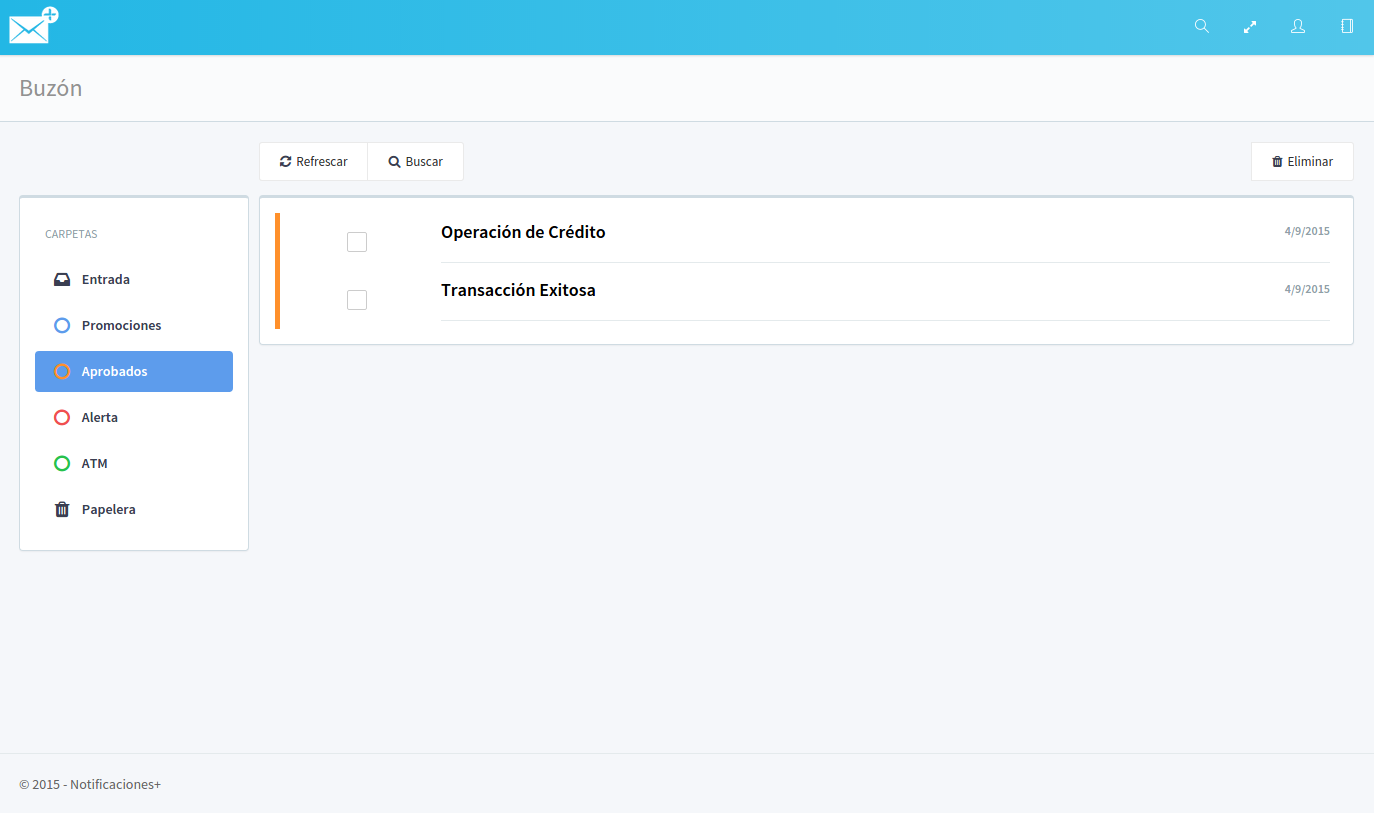
\includegraphics[width=11cm]{imagenes/Filtro2}}
  % \quad
  % \subfloat[Filtro Alerta]{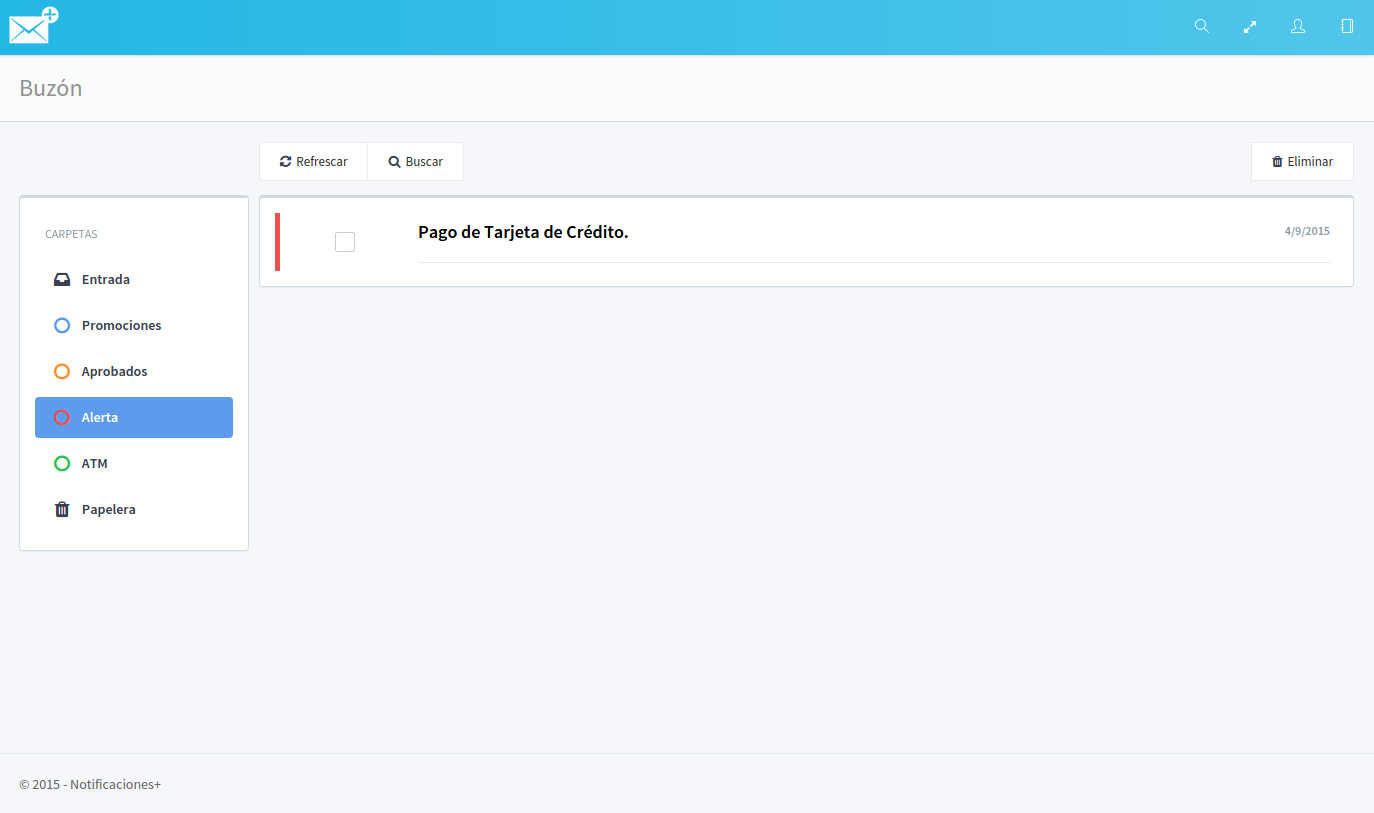
\includegraphics[width=11cm]{imagenes/Filtro3}}
  % \quad
  % \subfloat[Filtro ATM]{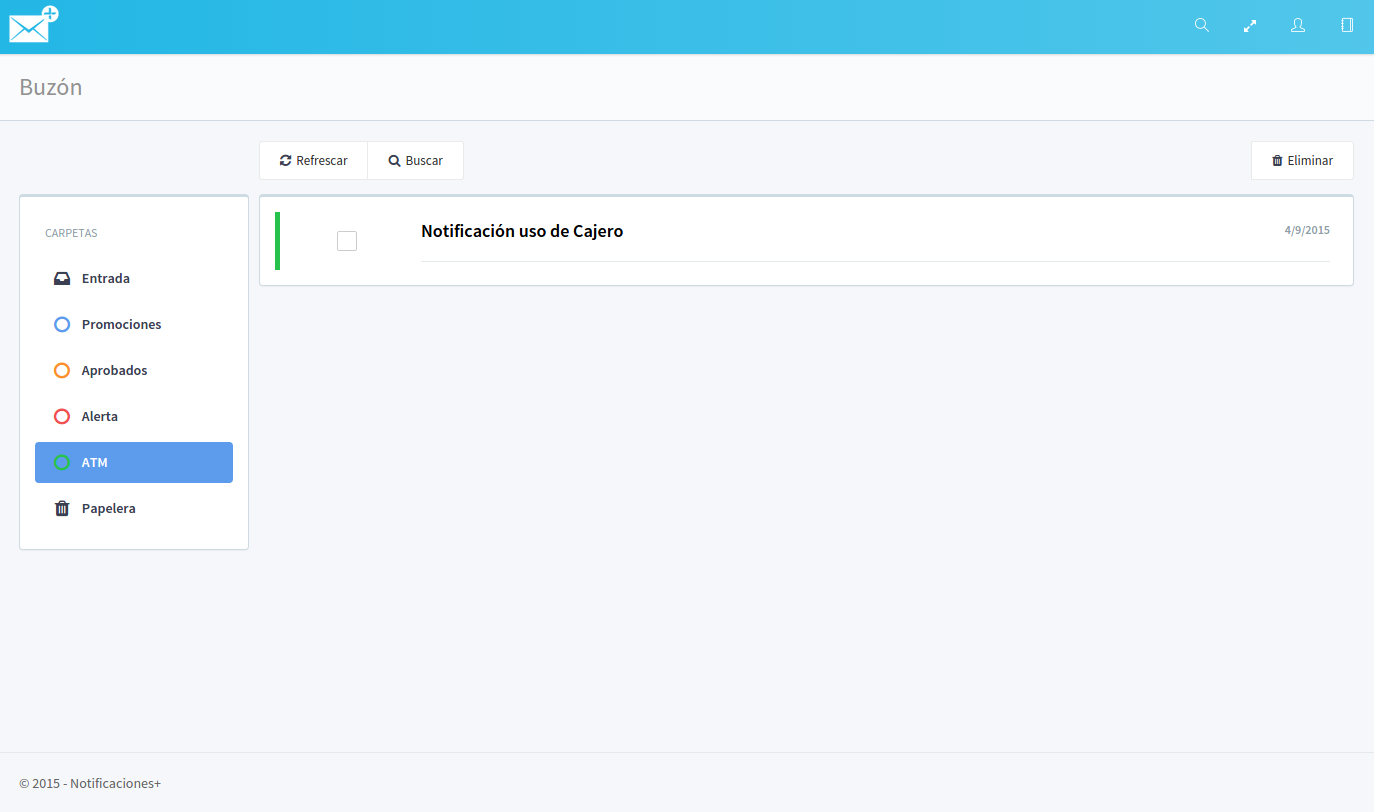
\includegraphics[width=11cm]{imagenes/Filtro4}} 
  % \quad
  \subfloat[Papelera]{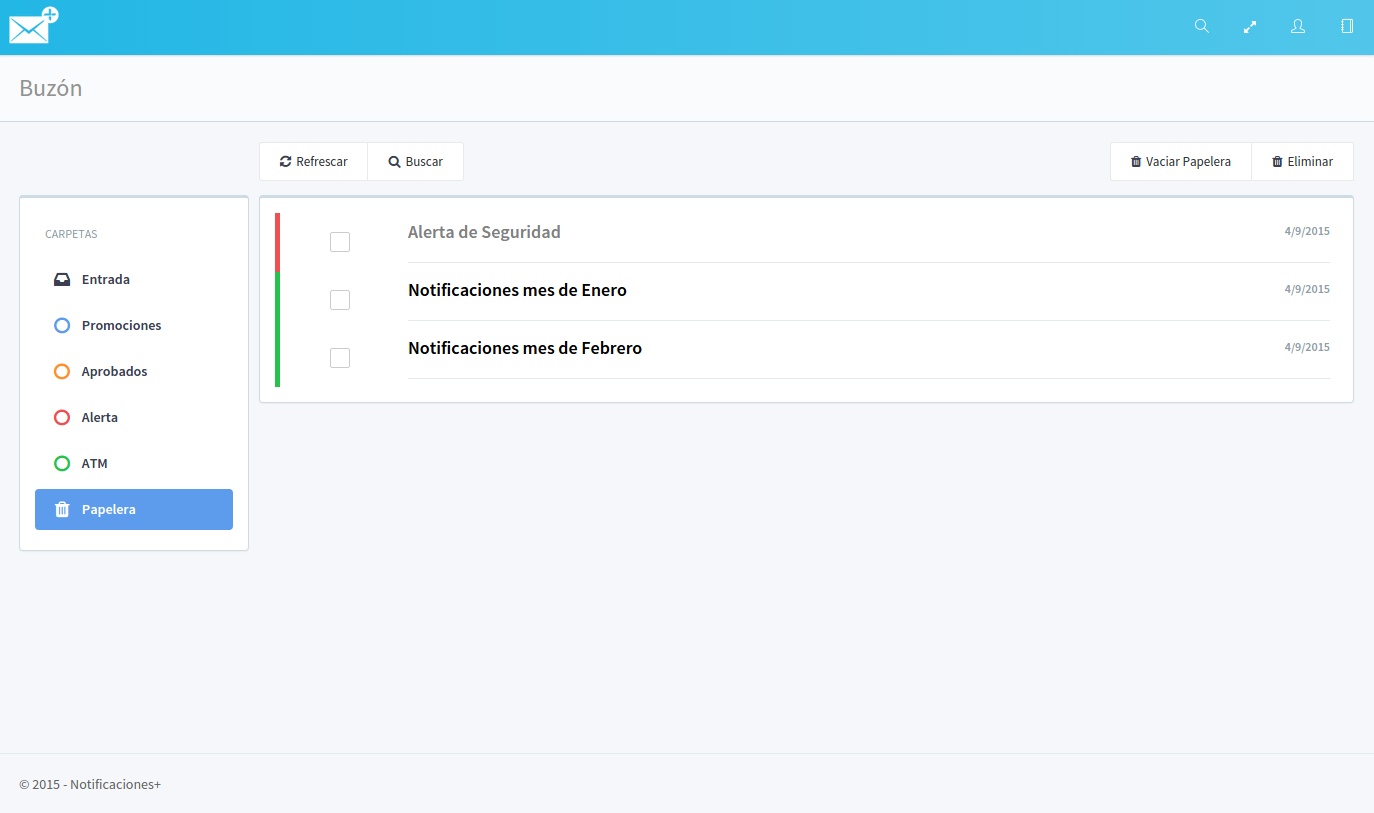
\includegraphics[width=11cm]{imagenes/Papelera}}
\caption{Pantalla de Buzón con botones de filtrado versión Web. Elaboración propia.}\label{fig:pantallaMultiWeb}
\end{figure}

% \begin{figure}[t]
% \centering
% \def\tabularxcolumn#1{m{#1}}
% \begin{tabularx}{\linewidth}{c}
% % 
%   \begin{tabular}{ccc}
%     \subfloat[Buzón de mensajes]{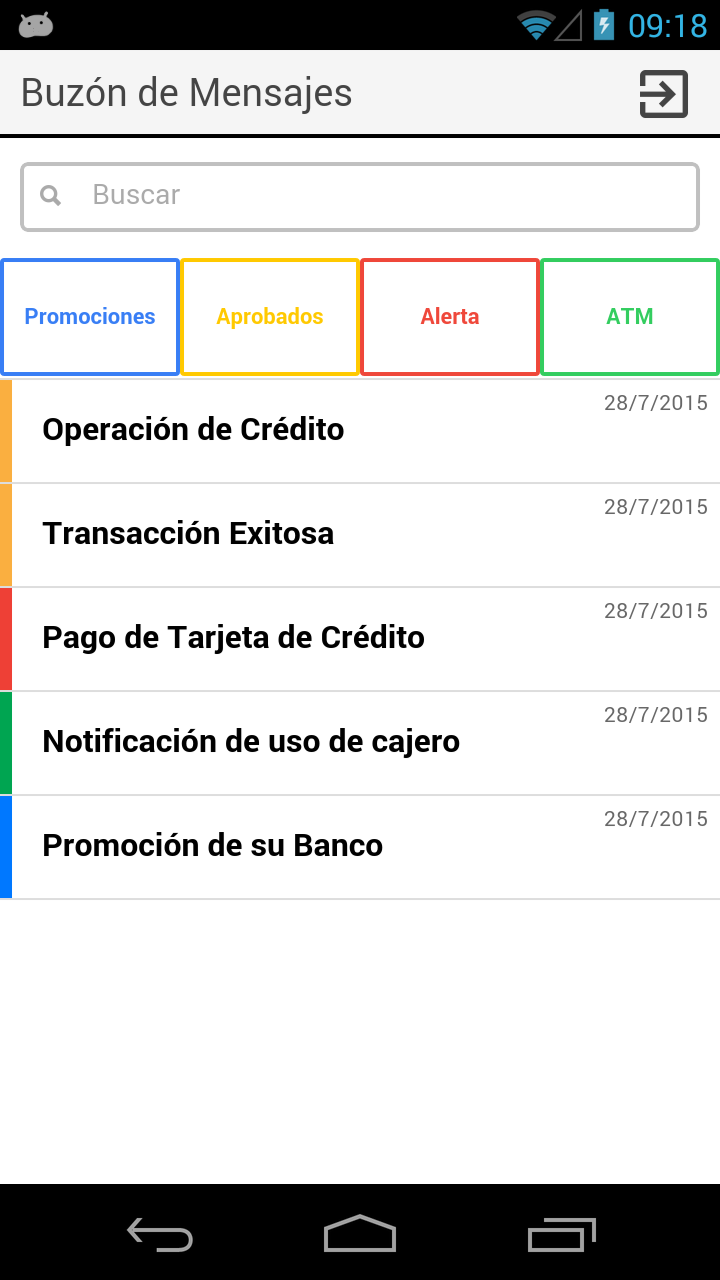
\includegraphics[width=3cm,type=png,ext=.png,read=.png,angle=0]{imagenes/pantalla5}} 
%     & \subfloat[Filtro Aprobados]{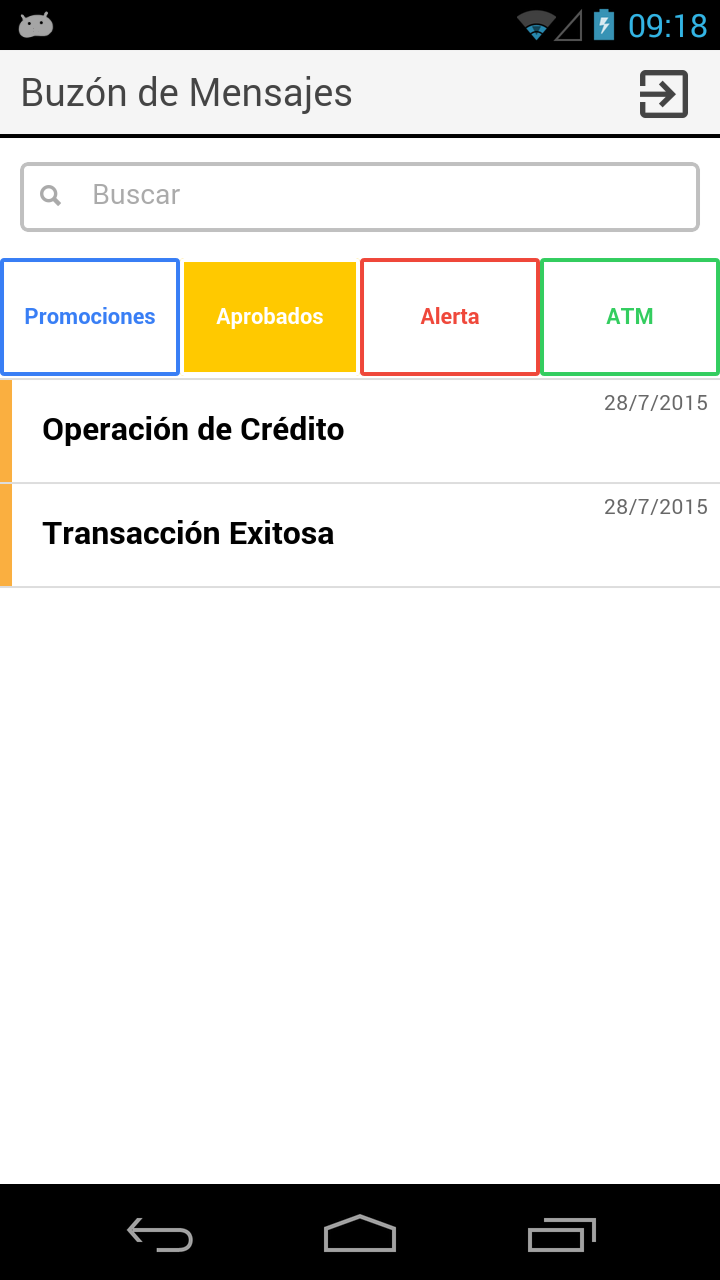
\includegraphics[width=3cm,type=png,ext=.png,read=.png,angle=0]{imagenes/pantalla6}}
%     & \subfloat[Filtro Promociones]{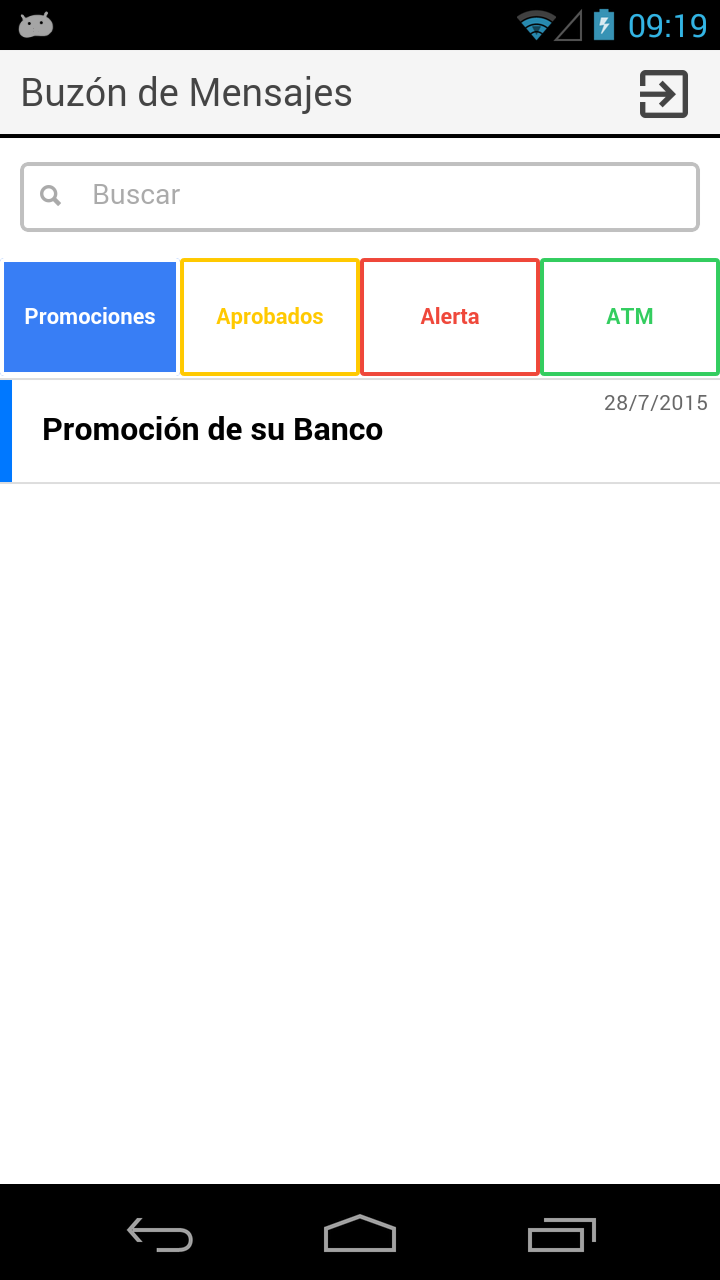
\includegraphics[width=3cm,type=png,ext=.png,read=.png,angle=0]{imagenes/pantalla7}}\\
%     \subfloat[Filtro Alerta]{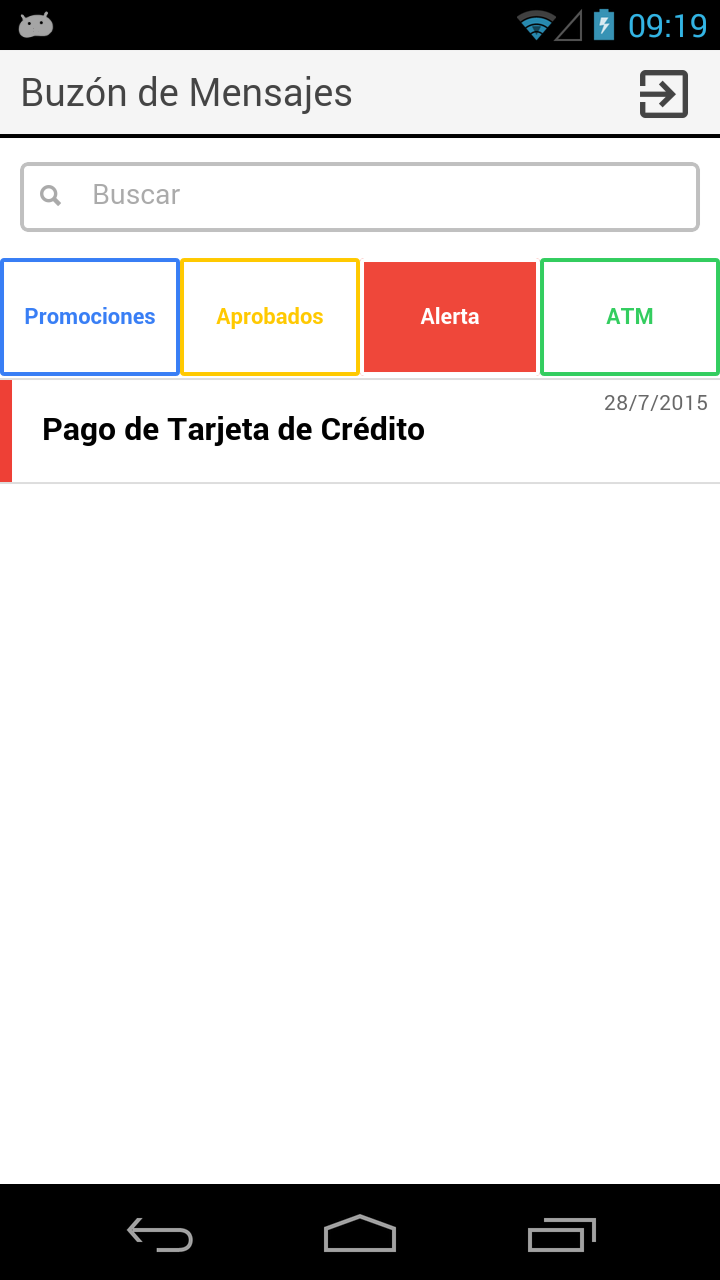
\includegraphics[width=3cm,type=png,ext=.png,read=.png,angle=0]{imagenes/pantalla8}}
%     & \subfloat[Filtro ATM]{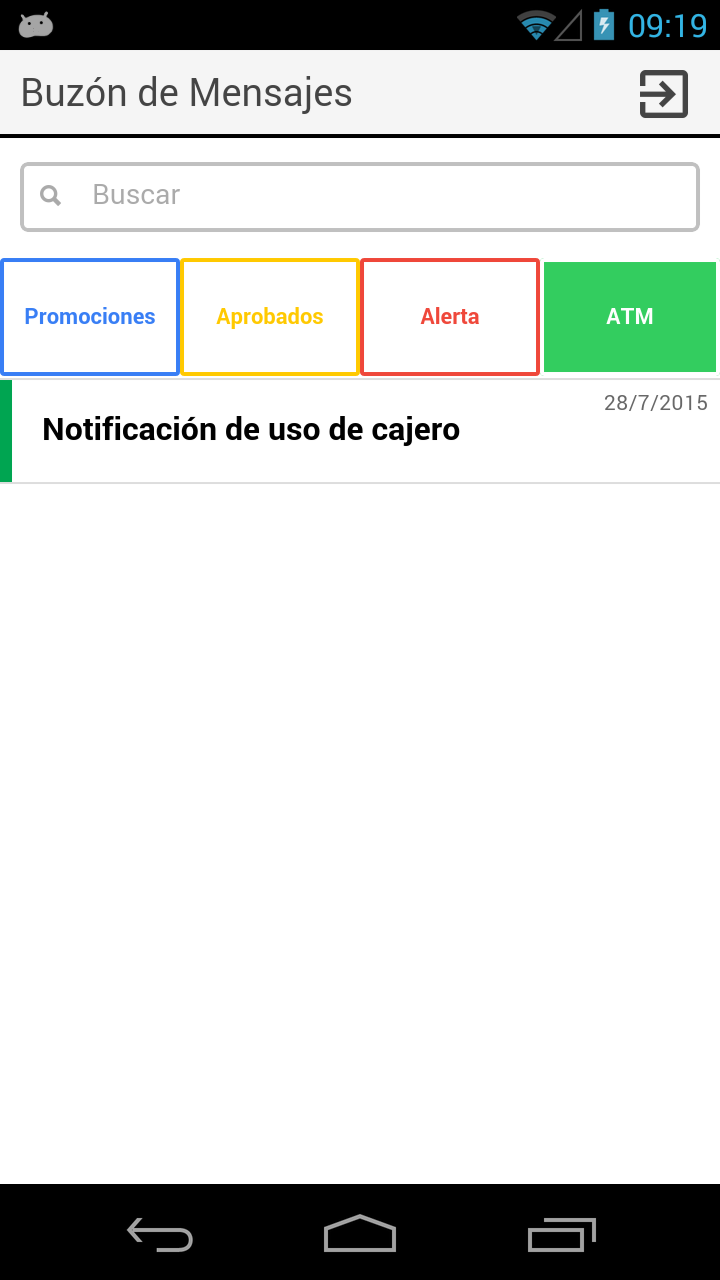
\includegraphics[width=3cm,type=png,ext=.png,read=.png,angle=0]{imagenes/pantalla9}} 
%     & \subfloat[Mensaje leído]{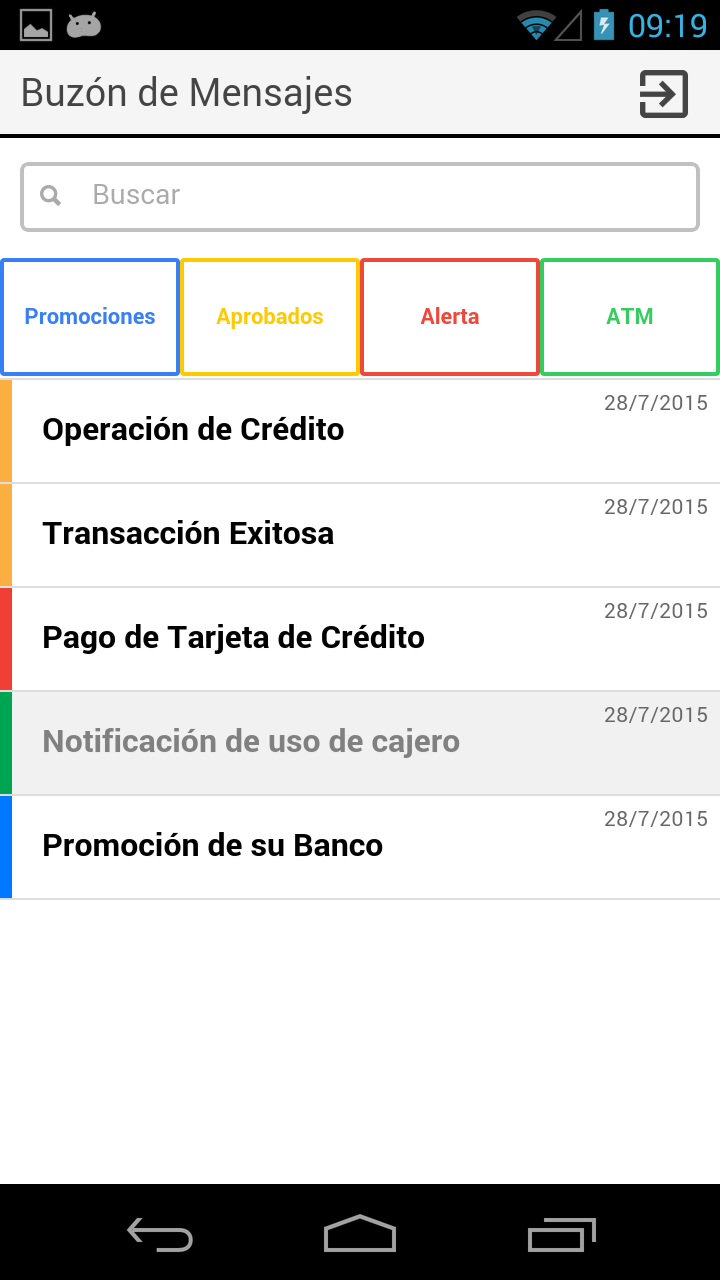
\includegraphics[width=3cm,type=png,ext=.png,read=.png,angle=0]{imagenes/pantalla10}}\\
%   \end{tabular}
% \end{tabularx}

% \caption{Pantalla de Buzón con botones de filtrado. Elaboración propia.}\label{fig:pantallaMulti}
% \end{figure}

Al deslizar un mensaje hacia la izquierda se muestra los botones de opcíon de compartir y eliminar. De seleccionarse eliminar se mostrará un menú de confirmación. El aspecto de los menús de confirmación y de las opciones para compartir dependen de la plataforma de la aplicación (iOS o Android). Ver la Figura ~\ref{fig:pantallaMulti2}.

\begin{figure}[htp]
\centering
  \subfloat[Opciones de mensaje]{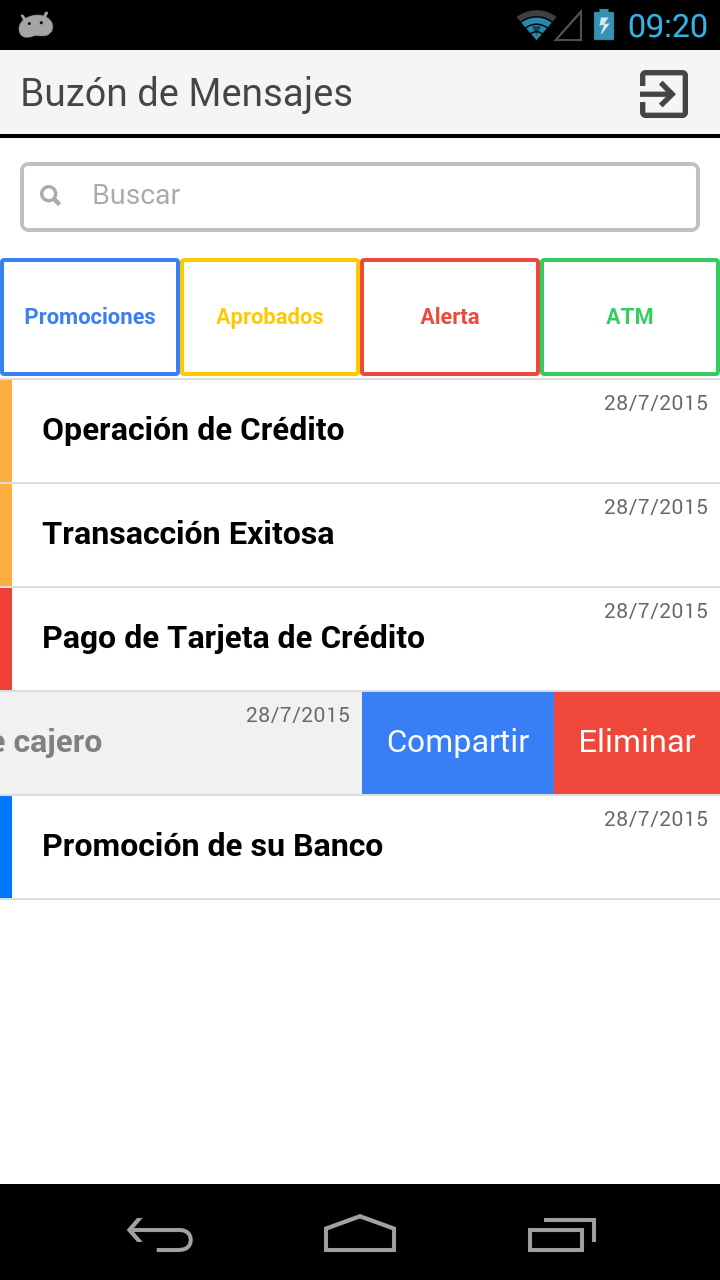
\includegraphics[width=3.5cm]{imagenes/pantalla11}} 
  \quad
  \subfloat[Confirmación de eliminar (Android)]{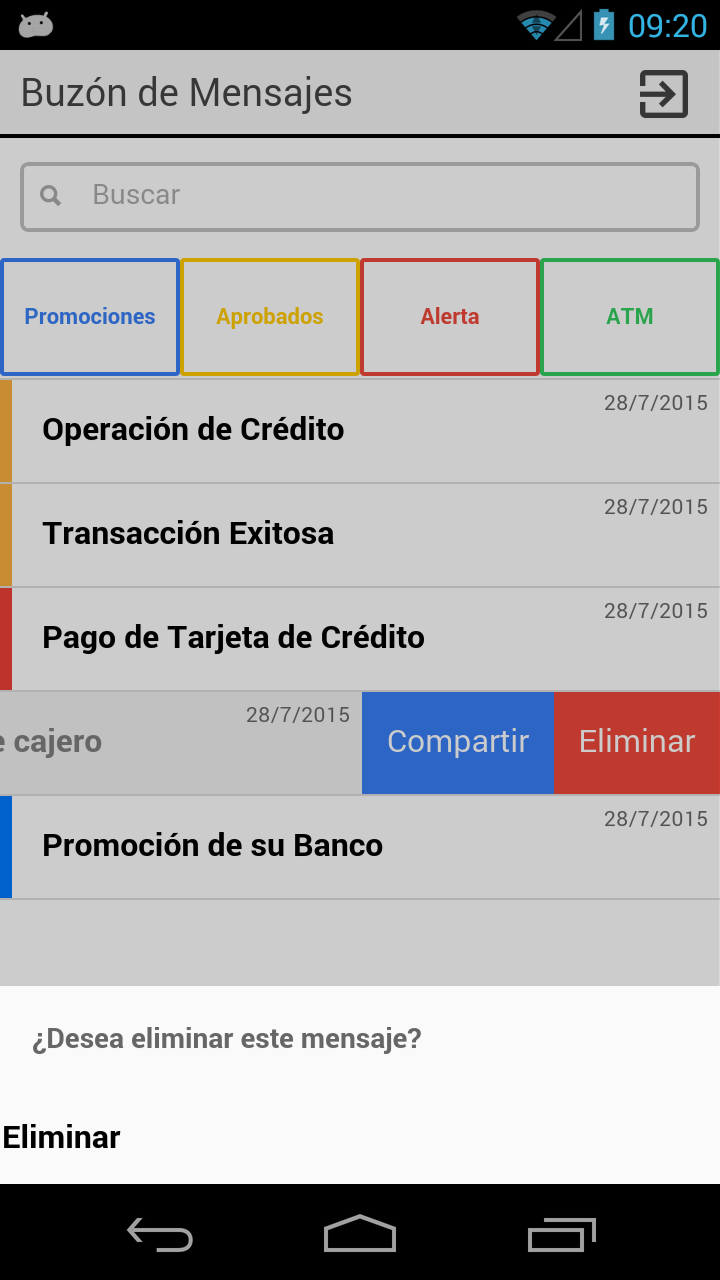
\includegraphics[width=3.5cm]{imagenes/pantalla12}}
  \quad
  \subfloat[Confirmación de eliminar (iOS)]{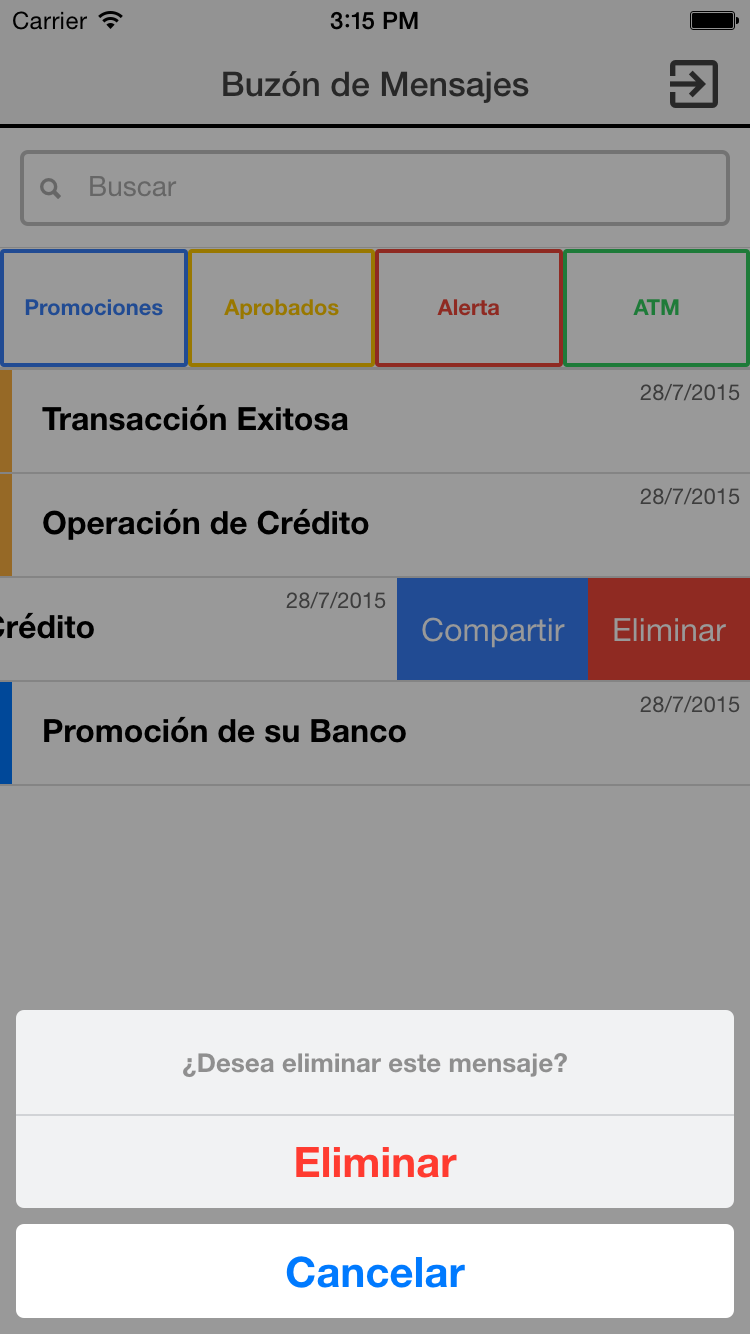
\includegraphics[width=3.5cm]{imagenes/iOSelim}}
\caption{Pantalla de Buzón con opciones de mensaje. Elaboración propia.}\label{fig:pantallaMulti2}
\end{figure}

% \begin{figure}[htp]
% \centering

% \subcaptionbox{Opciones de mensaje}{%
%   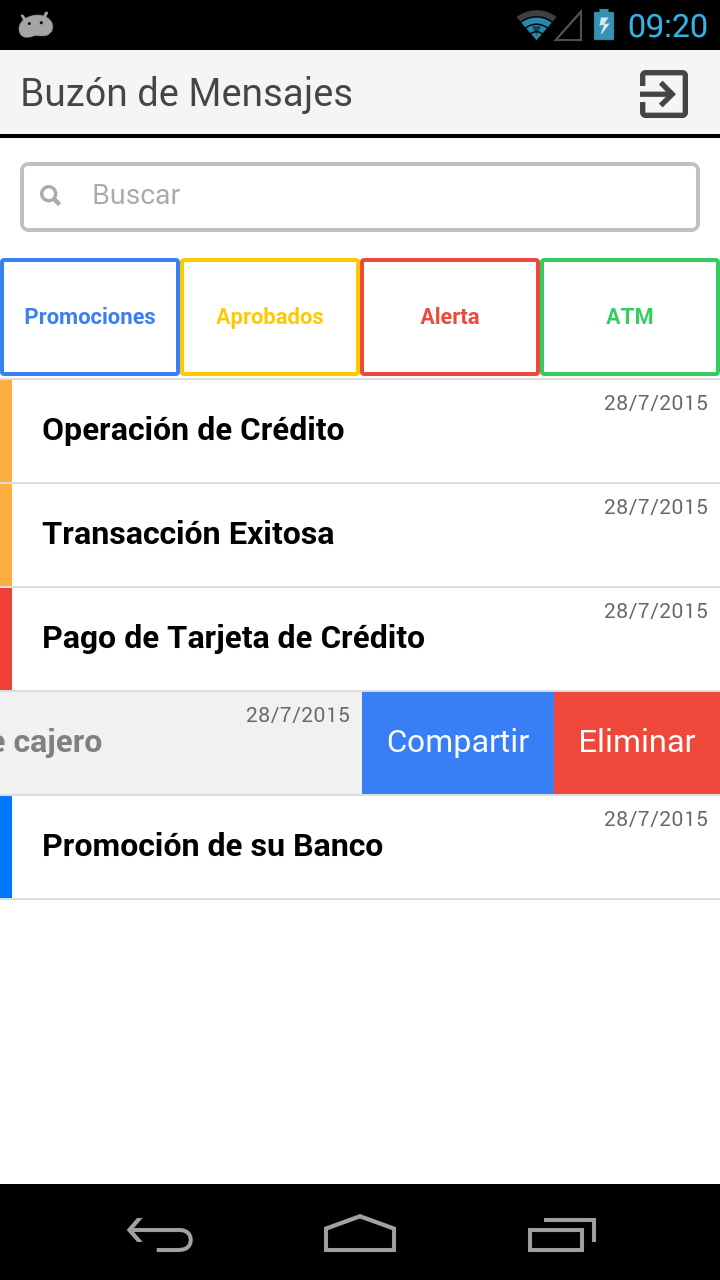
\includegraphics[width=3cm]{imagenes/pantalla11}%
% }\quad
% \subcaptionbox{Confirmación de eliminar (Android)}{%
%   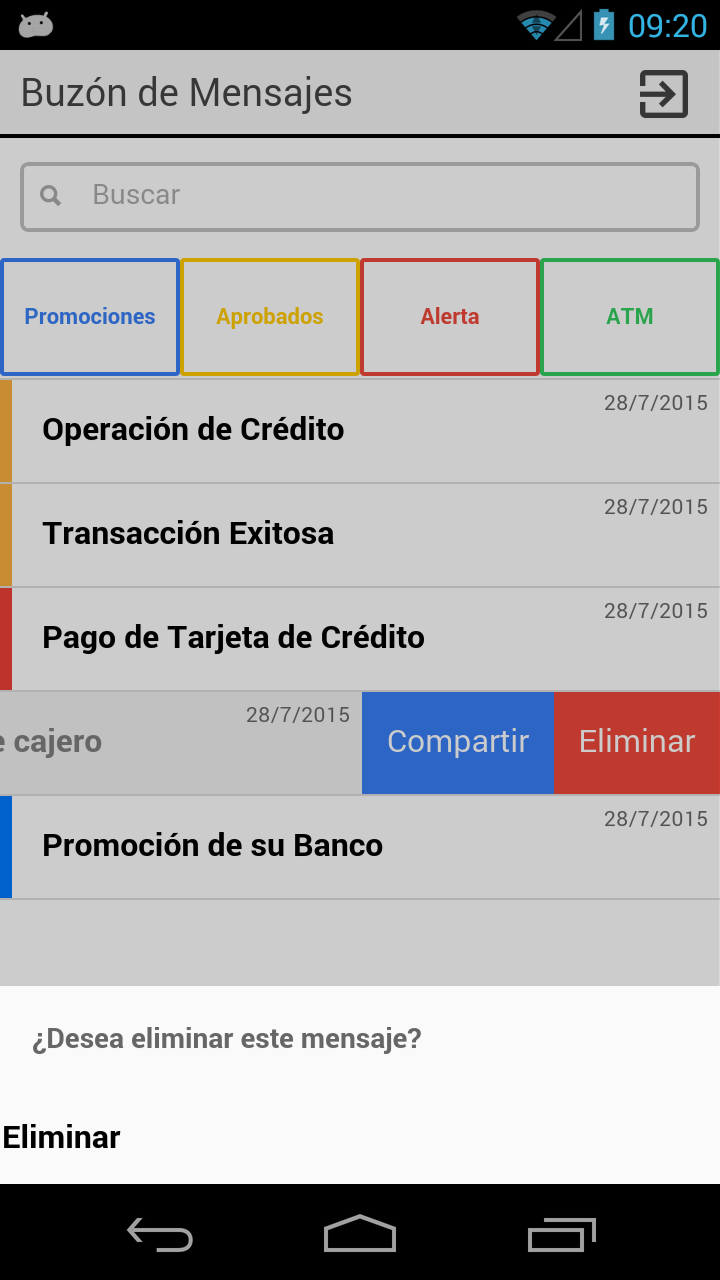
\includegraphics[width=3cm]{imagenes/pantalla12}%
% }\quad
% \subcaptionbox{Confirmación de eliminar (iOS)}{%
%   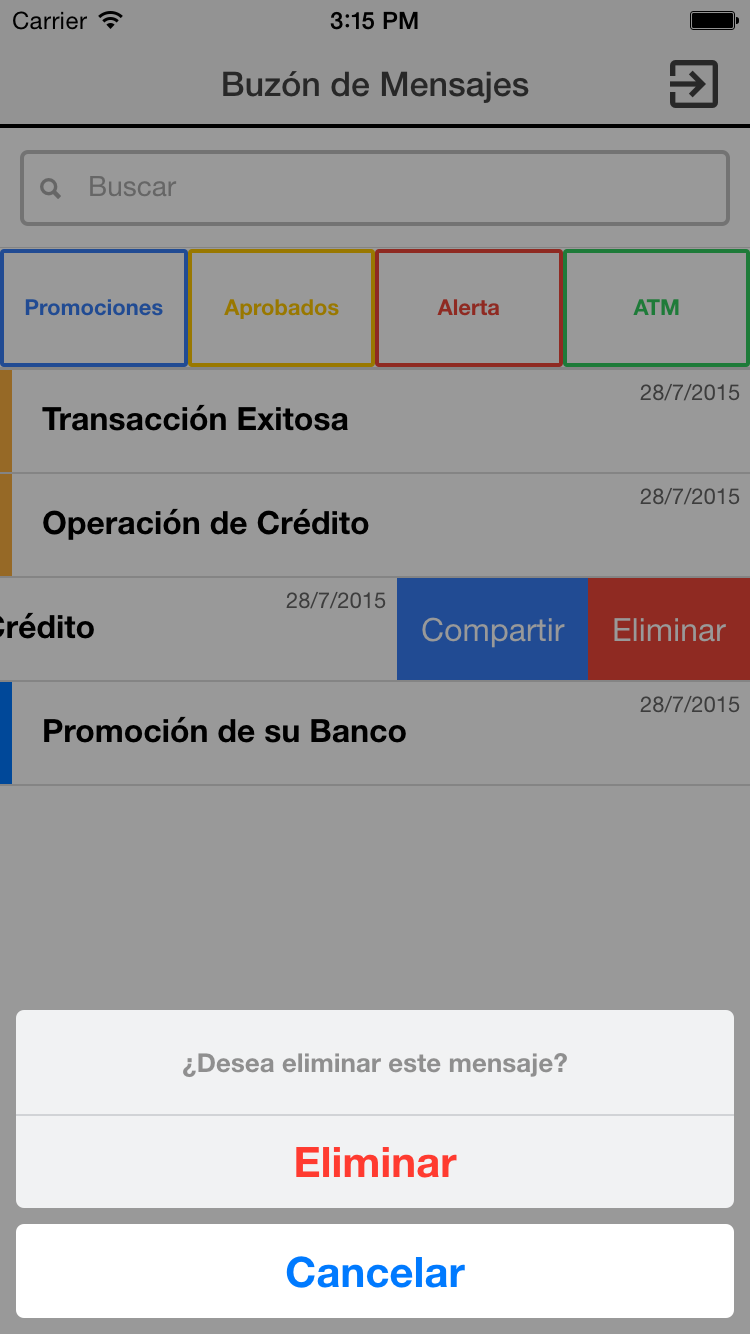
\includegraphics[width=3cm]{imagenes/iOSelim}%
% }

% \caption{Pantalla de Buzón con opciones de mensaje. Elaboración propia.}
% \label{fig:pantallaMulti2}

% \end{figure}

% \begin{figure}[t]
% \centering
% \def\tabularxcolumn#1{m{#1}}
% \begin{tabularx}{\linewidth}{c}
% %
%   \begin{tabular}{ccc}
%     \subfloat[Opciones de mensaje]{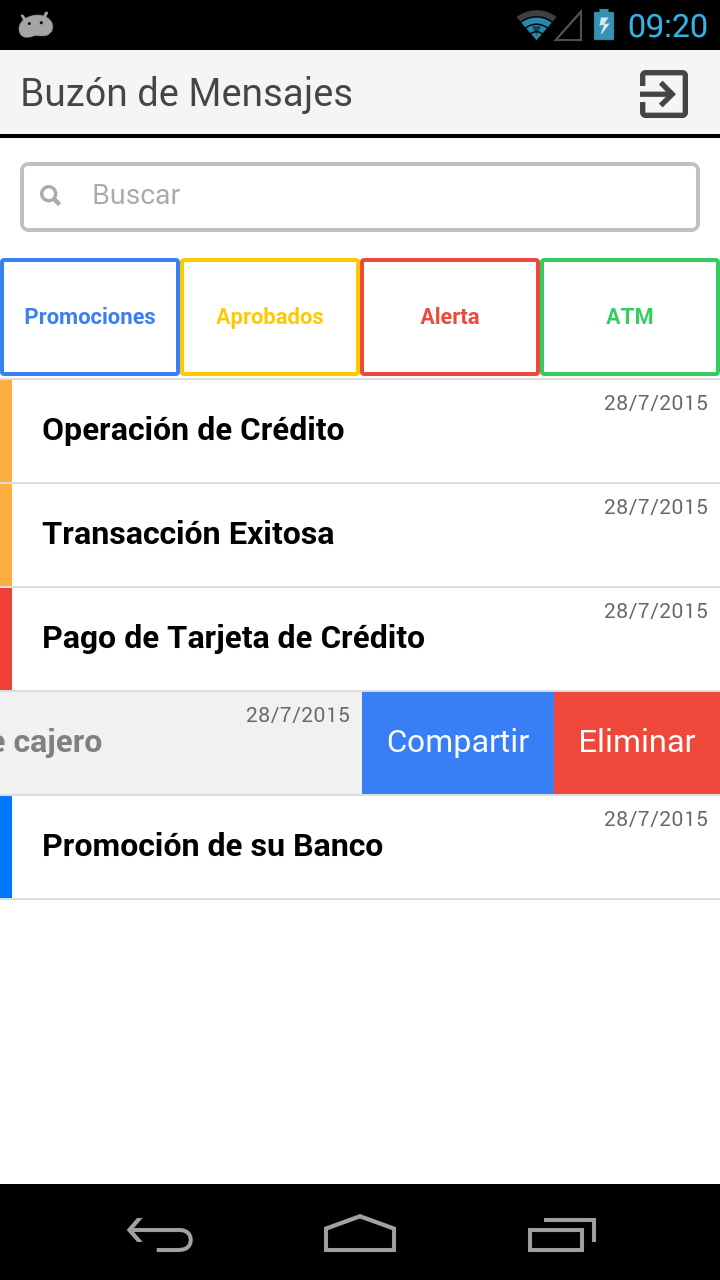
\includegraphics[width=3cm,type=png,ext=.png,read=.png,angle=0]{imagenes/pantalla11}} 
%     & \subfloat[Confirmación de eliminar (Android)]{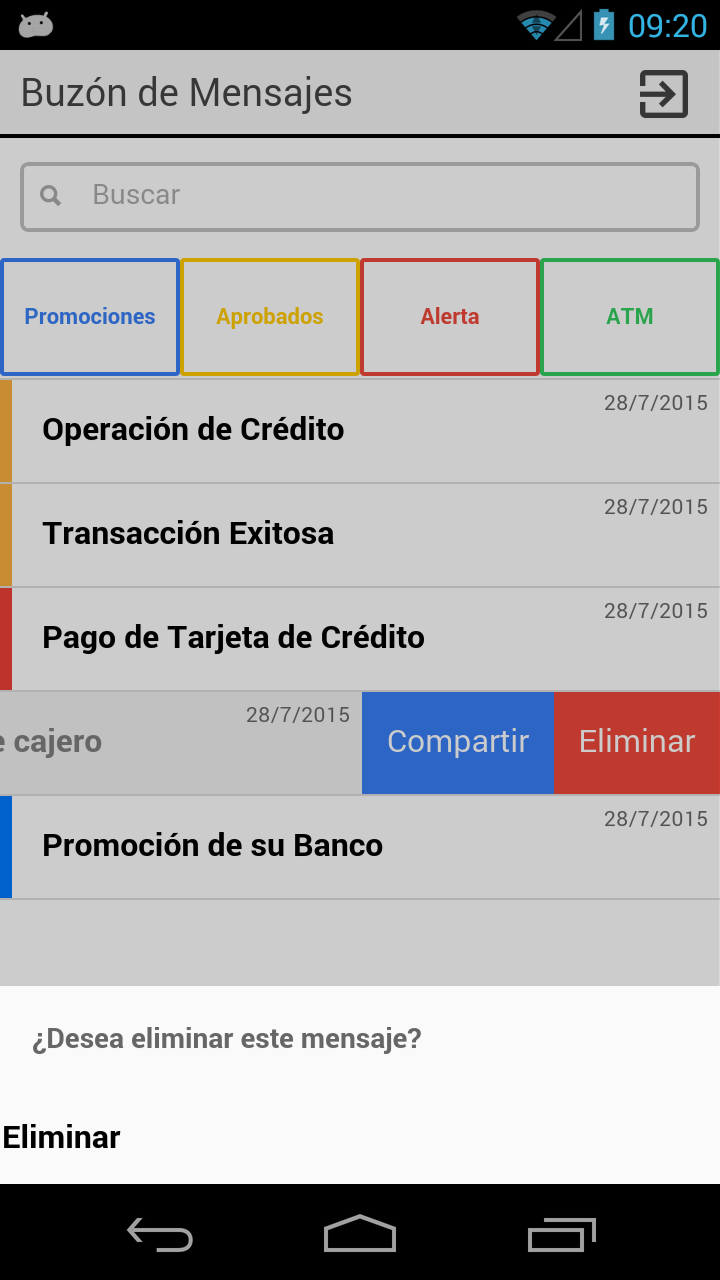
\includegraphics[width=3cm,type=png,ext=.png,read=.png,angle=0]{imagenes/pantalla12}}
%     & \subfloat[Confirmación de eliminar (iOS)]{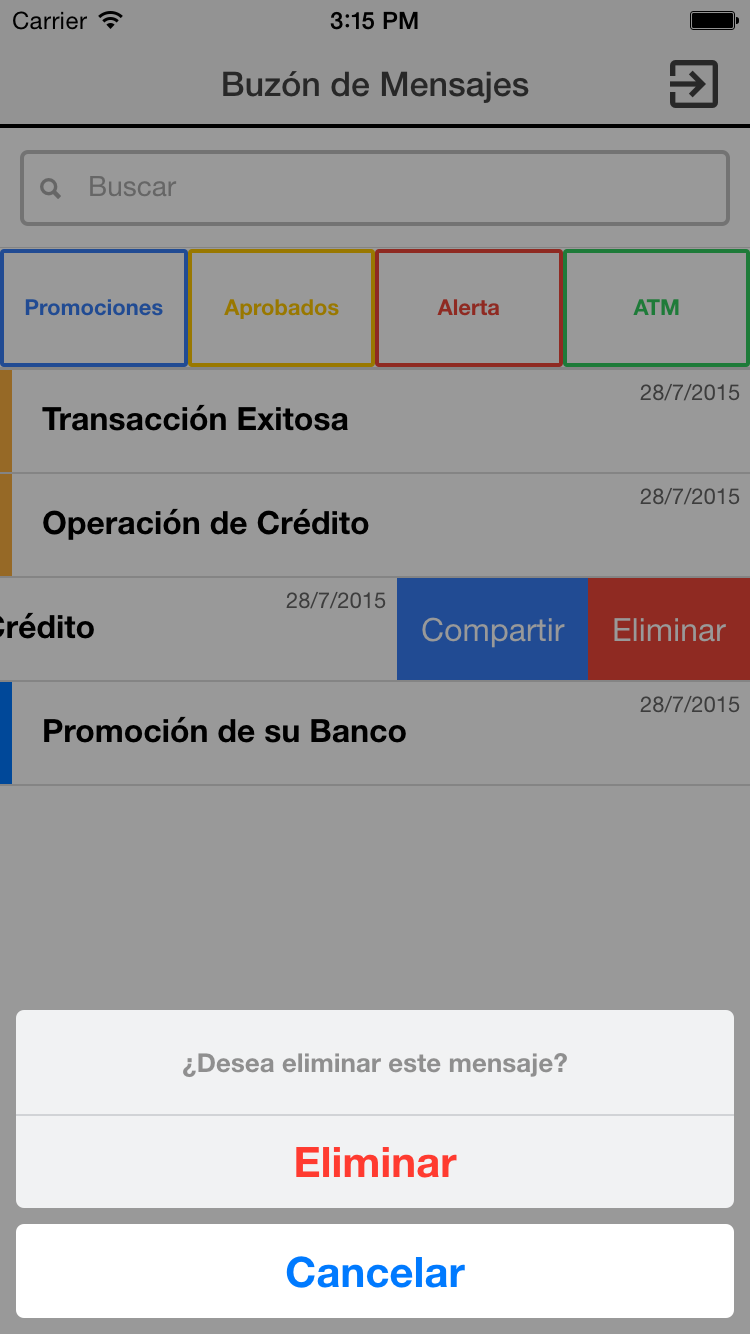
\includegraphics[width=3cm,type=png,ext=.png,read=.png,angle=0]{imagenes/iOSelim}}\\
%   \end{tabular}
% \end{tabularx}

% \caption{Pantalla de Buzón con opciones de mensaje. Elaboración propia.}\label{fig:pantallaMulti2}
% \end{figure}	

\section{Transición} \label{sect:Transicion}
La fase de transición no fue llevada a cabo debido a que el objetivo del proyecto fue, desde su concepción, la elaboración de un prototipo inicial 100\% funcional. Es por esto que tanto la aplicación web como la aplicación móvil de Notificaciones+ aún no ha entrado en una fase formal de transición a producción. Sin embargo, la plataforma Synergy Push (que provee los servicios de los que hace uso Notificaciones+) si se encuentra en producción y ya está siendo utilizada por bancos clientes de la empresa, así que la puesta en producción de Notificaciones+ dependería del momento en que la empresa quiera hacerlo.


\chapter{Retos Enfrentados y Logros Adicionales}\label{chapter:Retos y logros}

Este capítulo muestra aquellos retos que se presentaron a lo largo de la pasantía; así como la descripción de algunos logros adicionales que no estaban en el plan inicial.

\section{Retos enfrentados} \label{sect:Retos}
Durante el desarrollo del proyecto de pasantía surgieron una serie de retos considerables. El primer reto en presentarse fue el trabajar con una herramienta aún nueva, con la que solo un pasante había trabajado anteriormente, y que todavía está en su infancia en su desarrollo. Esto significó defectos y errores en la plataforma que dificultaran el aprendizaje y desarrolo además de poco soporte y documentación comparado con las plataformas nativas móviles.

Luego, la interfaz proporcionada por el departamento de diseño para la aplicación móvil constituyó un gran reto ya que, aunque la aplicación es simple, la interfaz de diseño minimalista contiene muchas particularidades que no son provistas por la plataforma Ionic. Por tanto se tuvieron que modificar estas y hacer trucos de programación para lograr los requerimientos visuales y funcionales de la interfaz. Hay dos casos en particular que cabe resaltar: los botones múltiples del menú principal y los botones filtros de la página buzón.

Los botones del menú principal fueron un reto en el sentido en que se requería una forma particular de los botones, no el estándar rectangular que provee Ionic, así que se tuvo que improvisar botones invisibles, parcialmnete solapados entre si, que estuvieran libre del contexto del resto de la página para colocarlos debajo de la imágen de botones provistas por el departamento de diseño para que funcionaran como se requería. Los botones filtros significaron tener que modificar la funcionalidad normal las cabeceras de página y de los botones provista por Ionic. Se tuvo que modificar la acción de los botones para que estos se quedaran presionados mientras ejercían su función como filtros, pero que a la vez solamente se permitiera uno presionado a la vez. Estos dos retos fueron superados gracias a la manipulación de las funcionalidades de AngularJS sobre HTML y CSS de la aplicación, con ideas provistas por la comunidad de StackOverflow.

Otro reto importante fue el mantener un buen desempeño de la aplicación, ya que posiblemente tenga que manejar grandes cantidades de mensajes. Por lo tanto se hizo uso de las herramientas que AngularJS ofrece para que la manipulación de mensajes (apertura, eliminación y guardado) sea lo más eficiente posible.


Posiblemente el reto más importante, no por su dificultad sino por lo crítico que era para la funcionalidad de la aplicación, era el uso del plugin para la recepción de notificaciones push en Cordova. Primero no se tenía mucho soporte ya que era un plugin nuevo, hecho por terceros ajenos a la plataforma Ionic, y se requirió mucho tiempo y ensayo y error para hacerlo funcionar. Después se descubrió un fallo: las notificaciones push provenientes de la plataforma Synergy Push no eran recibidas cuando la aplicación estaba en segundo plano. Se detectó el orígen del problema en un fallo del dieño del código fuente del plugin de Cordova, por lo que se tuvo que modificar el código fuente para solventarlo.


\section{Logros adicionales} \label{sect:Logros}
Durante el desarrollo del proyecto de pasantía se alcanzaron una serie de logros adicionales que no se encontraban estipulados en el plan de trabajo inicial. Entre ellos se encuentra la realización las maquetas iniciales que normalmente corresponderían al equipo de diseño o equipo encargado de planificar el producto, pero fue delegada al pasante que entregó al dueño del producto para su aprobación y luego al equipo de diseño para la fabricación de la interfaz definitiva. El dueño del producto especificó las funcionalidades que debía tener la aplicación y a partir de estos el pasante creó los casos de uso y luego las maquetas en base a esos casos. 

Para que el sistema de tipos de mensaje (Promoción, Aprobados, Alerta y ATM) y su clasificación (Respuesta Simple, Respuesta de dos Opciones, o WebView) funcionara, se tuvo que crear un estándar de identificación para que cada mensaje proveniente de Synergy Push estuviera debidamente identificado y la aplicación supiera identificarlos y tratarlos. Esto fue un logro adicional ya que la empresa no había decidido todavía como tratar a los mensajes. Solo estaba hecha la plataforma Synergy Push que trata mensajes genéricos y el concepto de la aplicación. Durante este trayecto se descubrió un error en la implementación de Synergy Push del cual la empresa no estaba al tanto, y fue informada para su futura corrección. Mientras estas se llevaban a cargo se implementó una solución provisional dentro de la aplicación que solventara el error contenido en los mensajes, haciendo uso de expresiones regulares.

Otro defecto encontrado de la plataforma Synergy Push es que actualmente envía los mensajes sin fecha, por lo que fue necesario agregarle a Notificaciones+ la funcionalidad de agregarle fecha a los mensajes cuando son recibidos.

La modificación del código fuente del plugin de recepción de notificaciones push de Cordova se cuenta como un logro adicional. El defecto del diseño de este plugin también fue reportado en su repositorio y en la comunidad de StackOverflow.

Finalmente, otro logro adicional fue la localización de otro error, pero esta vez es en la plataforma Ionic, que fue reportado a los creadores. La plataforma Ionic posee animaciones cuando manipula elementos en una lista, y uno de estas animaciones desencadena un error fatal cuando corre bajo la plataforma iOS 7. Para solventarlo se eliminó la animación exclusivamente en esa plataforma.


\chapter{Conclusiones y Recomendaciones} 

\label{chap:conclusiones}

En este proyecto de pasantía se desarrolló la aplicación web y móvil de Notificaciones+, donde sus objetivos es ofrecer a sus usuarios una manera de recibir y recopilar todas sus notificaciones bancarias como alertas de seguridad, promociones y transacciones de cajeros automáticos. El proceso completo incluyó el diseño y desarrollo de las aplicaciones, y su conexión con la plataforma de mensajería Synergy Push ya existente en la compañía.


Cabe acotar que las opciones y tipos de mensajes demostradas en esta aplicación a lo largo de todo el informe no son fijas y se pueden adaptar a las necesidades y preferencias de cualquier banco al que se le instancie la aplicación, incluso el cliente al que se le ofrezca la aplicación podría ser otro tipo de empresa diferente a un banco.


Para el momento de concepción de este proyecto no existía un competidor en el mercado venezolano, ya que todos los bancos notifican a sus clientes a través de mensajería SMS o e-mail.


Para poder lograr el proyecto, se usaron distintas herramientas entre las que se encuentran PhoneGap/Cordova, Ionic Framework y AngularJS para la aplicación móvil. Éstas permitieron su desarrollo sin necesidad de tener conocimientos específicos de ninguna plataforma móvil sino de programación web. Con el uso de buenas prácticas de programación para así lograr que la aplicación lograra un desempeño lo más similar posible a una aplicación nativa Android o iOS. AngularJS fue también la herramienta utilizada para desarrollar la aplicación web, usando adicionalmente Gulp para la automatización de tareas y una plantilla de aplicación web de la empresa.


Luego de 20 semanas de su inicio, al final del proyecto de pasantía, se obtuvo un prototipo funcional para la aplicación móvil. Cumple con todos los requerimientos hechos por el cliente en el plan inicial y también con las funcionalidades extras que surgieron durante el desarrollo, ideadas por el pasante como complemento a las requerimientos básicos originales con la intención de mejorar el producto final, guíandose del ejemplo de otras aplicaciones comunes que no están relacionadas a este proyecto.


A pesar de que el producto final de este proyecto cuenta con las aprobación del cliente, el pasante considera posibles futuras mejoras y ampliaciones que le darían a la empresa la posibilidad de hacer un producto más competitivo y atractivo a los posibles bancos y demás clientes que estén interesados en adquirir el producto. Estas ampliaciones son:
\smallskip
\begin{itemize}[noitemsep,nolistsep]
	\item Agregar una pantalla adicional para mensajes guardados. Ya que a pesar de que los filtros en el buzón de mensajes son muy útiles, y cualquier mensaje abierto no borrado es un mensaje guardado, podría convertirse en un volumen incómodo y desagradable para el usuario.  
	\item Ampliar la información mostrada en el item de mensajes en la pantalla buzón.
	\item Agregar la habilidad de agregar archivos PDF a los mensajes, como alternativa a los mensajes Web View, para así poder mandar información como recibos de cajero y de transacciones a los mensajes y tenerlos guardados sin necesidad de poseer siempre una conexión a Internet.
	\item A medida de que la plataforma Ionic crezca, instanciar la aplicación a Windows Phone además de Android y iOS.
	\item A pesar de no ser necesario actualmente, se podría cambiar el guardado de mensajes actual simple agregando una base de datos, para así poder guardar eficientemente información necesaria en futuras ampliaciones. En su estado actual la aplicación no necesita una base de datos ya que solo guarda el texto de los mensajes, pero si se agregan funcionalidades adicionales podría ser necesaria.
\end{itemize}
\bigskip

Se recomienda enormemente para la salida a producción de Notificaciones+ corregir los problemas de la plataforma Synergy Push, ya que evitaría posibles futuros conflictos dentro de la aplicación y además le quitaría carga de procesamiento que usa para corregir el defecto. También se le debe agregar a los mensajes provenientes de Synergy Push la \textit{fecha de envío}, así la aplicación no tiene que agregarles fecha que sería realmente la \textit{fecha de recibo}.


Por último se recomienda que se realicen pruebas exhaustivas que garanticen la calidad de la aplicación, incluyendo pruebas de capacidad de carga y desempeño para ver que tan capaz es una aplicación hecha en Ionic para manejar grandes cantidades de mensajes. Además de probar la aplicación en distintos dispositivos con diferentes tamaños y versiones de sistema operativo, sobre todo en la plataforma Android.


La experiencia de la pasantía permitió al pasante poner en práctica los conocimientos adquiridos a lo largo del periodo universitario para solventar un problema real, así como aprender nuevas herramientas y tecnologías como servicios web REST, de los cuales el pasante no sabía su existencia hasta entrar en contacto con Synergy. Aunque no se generaron servicios web si se trabajó con ellos. También se generó un crecimiento en cuando a la gestión del tiempo, gestión de los cambios en los requerimientos y estimación del tiempo que llevaría realizar alguna actividad. Adicionalmente, el pasante tuvo la oportunidad de trabajar sobre una arquitectura con muchos conceptos e innovaciones. Ionic y AngularJS son herramientas que tienen muchas aplicaciones y mucho futuro. Esta experiencia resultó muy beneficiosa para el pasante ya que no solo aumenta sus destrezas y habilidades en el ámbito laboral, sino que lo introdujo al mundo de aplicaciones y programación web y móvil, lo cual era su objetivo principal al aceptar la pasantía en Synergy.

  
Finalmente, a los futuros pasantes se les recomienda definir claramente el alcance y los requerimientos al comenzar la pasantía y mantener reuniones periódicas con el cliente o responsable del proyecto en la empresa para que el mismo apruebe lo desarrollado hasta el momento. Así mismo, se recomienda estudiar las buenas prácticas utilizadas por la empresa y tomarlas en cuenta a lo largo del desarrollo, utilizar patrones de diseño de \textit{software} en caso de ser posible y consultar la documentación de las herramientas para sacar todo el provecho posible de las mismas. Tener siempre en cuenta las buenas prácticas de programación aprendidas en la carrera universitaria; tener paciencia al tratar con una plataforma nueva, ya que es algo que un ingeniero de computación o \textit{software} va a tener que hacer durante toda su vida; ser ordenado y competente, siempre apuntando a la mejor manera de hacer las cosas. 






% % Establece las citas y bibliografia
\bibliographystyle{ieeetr}
\bibliography{myrefs}

\glsaddall
\printglossary

% % Crea el apendice
\appendix
% \chapter{Lista de Riesgos}
% \includepdf[pages=-]{apendices/ListaRiesgos.pdf}
\chapter{Documento de Arquitectura de Software}
\includepdf[pages=-]{apendices/DAS.pdf}
\chapter{Especificación Funcional}
\includepdf[pages=-]{apendices/ERS.pdf}
% \chapter{Investigación de la Arquitectura Banca+ Multicanal}
% \includepdf[pages=-]{apendices/ArquitecturaBanca+Multicanal.pdf}
% \chapter{Arquitectura de Servicios Web REST}
% \includepdf[pages=-]{apendices/REST.pdf}
\chapter{Sprint Backlog}
\includepdf[pages=-]{apendices/SprintBacklog.pdf}
%\includepdf[pages=-]{apendices/IFFv1.1/IFF.pdf}
%%\documentclass[12pt,letterpaper]{article}
%\usepackage[utf8]{inputenc}
%\usepackage{amsmath}
%\usepackage{amsfonts}
%\usepackage{amssymb}
%\usepackage[spanish]{babel}
%\usepackage{array}
%\usepackage{longtable}
%\author{Jon Ander Ricchiuti}
%\title{IFF v1.1}
%\begin{document}
%\pagenumbering{arabic}
%\maketitle
%\thispagestyle{empty}
%\newpage
\chapter{Intercambio de Información Financiera (IFF)}

\section*{Introducción}

El protocolo de intercambio de información financiera (IFF), describe la forma correcta de comunicación con un prototipo de sistema bancario creado en Synergy Global Business (SGB). El IFF busca estandarizar el intercambio de información financiera que realizará el prototipo bancario. De esta manera la comunicación es sencilla y a la vez robusta. Para la realización de este protocolo de comunicación se utilizó como base el IFX (Interactive Financial Exchange).
\\
\\ 
La forma de comunicación que el IFF	utiliza es de tipo petición-respuesta (request-response). En cada petición se debe especificar un método. Este método define la naturaleza de la petición.
%\pagenumbering{arabic}
%\newpage

\section{Tipo de datos}

Los tipos de datos que se utilizarán en este estándar son los siguientes:
\begin{itemize}
\item Cadena de caracteres.
\item Enumeración.
\item Tiempo y Hora.
\item Entero.
\item Decimal
\item Booleano.
\end{itemize}

\subsection{Cadena de caracteres}
Las cadenas de caracteres se representan con el nombre de ``Cadena de caracteres'' seguido de la longitud de la misma. Esta longitud es representada entre paréntesis de la siguiente forma.
\begin{itemize}
\item Cadena de caracteres (X-Y), indica que la longitud mínima de la cadena de caracteres es ``X'' y la máxima longitud es ``Y''.
\item Cadena de caracteres (X+), indica que la longitud mínima de la cadena de caracteres es ``X'' pero no tiene longitud máxima para la misma.
\end{itemize}
Si la longitud no es especificada entonces no existe restricción sobre el tamaño de la cadena de caracteres.

\subsection{Enumeración}
Son los valores que puede tomar un campo. Estos pertenecen a un conjunto de cadena de caracteres definidas específicamente para ese campo en particular. Los diferentes tipos de enumeración serán especificados en la siguiente sección.

\subsection{Tiempo y Hora}
Tanto la hora como la fecha son cadenas de caracteres que se representan con un fromato particular. Para la hora el formto es ``\%H:\%M:\%S''. Para la fecha el formato es ``\%Y-\%m-\%d \%H:\%M:\%S''. Donde \%Y representa el año, \%m el mes, \%d el dia, \%H la hora, \%M el minuto, \%S el segundo. Todos los componentes de la hora y fecha se representan con caracteres numéricos.

\subsection{Entero}
Es un número entero y puede representarse de dos formas diferentes. Como un entero de cuatro bytes o como un entero de ocho bytes. Para especificar que es un entero de ocho bytes, debe ser escrito de la siguiente forma: Entero(8).
\\
\\
Si no se especifica que un entero es de ocho bytes entonces se asume que es de cuatro  bytes.

\subsection{Decimal}
Es un número con hasta quince dígitos decimales.

\subsection{Booleano}
Un Booleano representa si una condición se cumple o no. En el caso del IFF un Booleano será representado por medio de un carácter. Es decir, el carácter 'T' será el que representa cuando un estado es cierto y 'F' será el valor de cuando el estado no se cumple.

\section{Tipos de Enumeración}
\subsection{Correspondiente a personVerifyType}
\begin{center}
\begin{tabular}{|>{\centering\arraybackslash}p{0.3\textwidth}|>{\centering\arraybackslash}p{0.3\textwidth}|>{\centering\arraybackslash}p{0.3\textwidth}|}
\hline 
\bfseries {Valor} & \bfseries {Descripción} & \bfseries {Por defecto} \\ 
\hline 
Passport & Pasaporte de crédito & N \\ 
\hline 
CI & Cedula de identidad & N \\
\hline 
\end{tabular} 
\end{center}

\subsection{Correspondiente a nameAddrType}
\begin{center}
\begin{tabular}{|>{\centering\arraybackslash}p{0.3\textwidth}|>{\centering\arraybackslash}p{0.3\textwidth}|>{\centering\arraybackslash}p{0.3\textwidth}|}
\hline 
\bfseries {Valor} & \bfseries {Descripción} & \bfseries {Por defecto} \\ 
\hline 
Customer & Es la dirección del cliente & N \\ 
\hline 
ShipTo & Dirección a la cual algo debería ser enviado por correo & N \\
\hline 
Delivery & Dirección a la cual serán enviadas las facturas en papel & N \\
\hline 
\end{tabular} 
\end{center}

\subsection{Correspondiente a addrType}
\begin{center}
\begin{tabular}{|>{\centering\arraybackslash}p{0.3\textwidth}|>{\centering\arraybackslash}p{0.3\textwidth}|>{\centering\arraybackslash}p{0.3\textwidth}|}
\hline 
\bfseries {Valor} & \bfseries {Descripción} & \bfseries {Por defecto} \\ 
\hline 
Seasonal & Habitación vacacional & N \\ 
\hline 
Primary & Habitación principal & N \\
\hline 
Secondary & Habitación secundaria & N \\
\hline
Business & Dirección de negocio & N \\
\hline 
\end{tabular} 
\end{center}

\subsection{Correspondiente a cardStatusCode}
\begin{center}
\begin{tabular}{|>{\centering\arraybackslash}p{0.3\textwidth}|>{\centering\arraybackslash}p{0.3\textwidth}|>{\centering\arraybackslash}p{0.3\textwidth}|}
\hline 
\bfseries {Valor} & \bfseries {Descripción} & \bfseries {Por defecto} \\ 
\hline 
Active & Activa & N \\ 
\hline 
Expired & Vencida & N \\
\hline 
Blocked & Bloqueada & N \\
\hline
\end{tabular} 
\end{center}

\subsection{Correspondiente a accountStatusCode}
\begin{center}
\begin{tabular}{|>{\centering\arraybackslash}p{0.3\textwidth}|>{\centering\arraybackslash}p{0.3\textwidth}|>{\centering\arraybackslash}p{0.3\textwidth}|}
\hline 
\bfseries {Valor} & \bfseries {Descripción} & \bfseries {Por defecto} \\ 
\hline 
Active & Activa & N \\ 
\hline 
Blocked & Bloqueada & N \\
\hline
\end{tabular} 
\end{center}

\subsection{Correspondiente a cardType}
\begin{center}
\begin{tabular}{|>{\centering\arraybackslash}p{0.3\textwidth}|>{\centering\arraybackslash}p{0.3\textwidth}|>{\centering\arraybackslash}p{0.3\textwidth}|}
\hline 
\bfseries {Valor} & \bfseries {Descripción} & \bfseries {Por defecto} \\ 
\hline 
Credit & Tarjeta de crédito & N \\ 
\hline 
Debit & Tarjeta de débito & N \\
\hline 
\end{tabular} 
\end{center}

\subsection{Correspondiente a brand}
\begin{center}
\begin{tabular}{|>{\centering\arraybackslash}p{0.3\textwidth}|>{\centering\arraybackslash}p{0.3\textwidth}|>{\centering\arraybackslash}p{0.3\textwidth}|}
\hline 
\bfseries {Valor} & \bfseries {Descripción} & \bfseries {Por defecto} \\ 
\hline 
Visa &  & N \\ 
\hline 
MasterCard &  & N \\
\hline 
\end{tabular} 
\end{center}

\subsection{Correspondiente a transType}
\begin{center}
\begin{tabular}{|>{\centering\arraybackslash}p{0.3\textwidth}|>{\centering\arraybackslash}p{0.3\textwidth}|>{\centering\arraybackslash}p{0.3\textwidth}|}
\hline 
\bfseries {Valor} & \bfseries {Descripción} & \bfseries {Por defecto} \\ 
\hline 
Withdrawal & Retiro & N \\ 
\hline 
Deposit & Deposito & N \\
\hline 
Transference & Transferencia & N \\
\hline
\end{tabular} 
\end{center}

\subsection{Correspondiente a acctType}
\begin{center}
\begin{tabular}{|>{\centering\arraybackslash}p{0.3\textwidth}|>{\centering\arraybackslash}p{0.3\textwidth}|>{\centering\arraybackslash}p{0.3\textwidth}|}
\hline 
\bfseries {Valor} & \bfseries {Descripción} & \bfseries {Por defecto} \\ 
\hline 
Saving & Ahorro & N \\ 
\hline 
Current & Corriente & N \\
\hline 
Loan & Préstamo & N \\
\hline
\end{tabular} 
\end{center}

\subsection{Correspondiente a contactInfo}
\begin{center}
\begin{tabular}{|>{\centering\arraybackslash}p{0.3\textwidth}|>{\centering\arraybackslash}p{0.3\textwidth}|>{\centering\arraybackslash}p{0.3\textwidth}|}
\hline 
\bfseries {Valor} & \bfseries {Descripción} & \bfseries {Por defecto} \\ 
\hline 
dayPhone & Teléfono de contacto durante el día & N \\
\hline 
evePhone & Teléfono de contacto durante la tarde & N \\
\hline 
dayFax & Fax de contacto durante el día & N \\
\hline
eveFax & Fax de contacto durante la tarde & N \\
\hline
emailAddr & Dirección de correo electrónica & N \\
\hline
\end{tabular} 
\end{center}
	
\section{Recursos}
El protocolo IFF esta basado en recursos. Los recursos son fuentes de información sobre las cuales se realizan las peticiones. Estos recursos son divididos en dos grandes grupos, los concretos y los abstractos.

\subsection{Recursos concretos}
Los recursos concretos son la representación directa del modelo de datos que expone el core bancario para ofrecer sus servicios. Este tipo de recursos es muy sencillo y son los que permiten realizar las operaciones más básicas. \\

A continuación se presentan los recursos concretos.

\subsubsection{Nombre de usuario ``login''}
Contiene la información que relaciona el nombre de usuario electrónico con su información  en la institución financiera.

\begin{center}
\begin{tabular}{|>{\centering\arraybackslash}p{0.2\textwidth}|>{\centering\arraybackslash}p{0.2\textwidth}|>{\centering\arraybackslash}p{0.2\textwidth}|>{\centering\arraybackslash}p{0.2\textwidth}|}
\hline 
\bfseries {Etiqueta} & \bfseries {Tipo} & \bfseries {Uso} & \bfseries {Descripción} \\ 
\hline 
username & Cadena de caracteres (6-20) & Requerido & ID de ingreso del cliente \\ 
\hline 
password & Cadena de caracteres (6+) & Opcional & Clave de ingreso \\ 
\hline 
custPermId & Cadena de caracteres (32+) & Requerido & ID permanente del cliente. Es asignado por la institución financiera para representar al cliente en el sistema \\ 
\hline 
\end{tabular}
\end{center}

\subsubsection{Cliente ``customer''}
Tiene la información que identifica inequívocamente a un cliente.

\begin{center}
\begin{longtable}{|>{\centering\arraybackslash}p{0.25\textwidth}|>{\centering\arraybackslash}p{0.2\textwidth}|>{\centering\arraybackslash}p{0.15\textwidth}|>{\centering\arraybackslash}p{0.2\textwidth}|}
\hline 
\bfseries {Etiqueta} & \bfseries {Tipo} & \bfseries {Uso} & \bfseries {Descripción} \\ 
\hline 
custPermId & Cadena de caracteres (32+) & Opcional & ID permanente del cliente. Es asignado por la institución financiera para representar al cliente en el sistema \\ 
\hline 
personId & Cadena de caracteres (32+) & Opcional & Relación al objeto ``person'' \\ 
\hline 
custLogin & Cadena de caracteres (6-20) & Opcional & ID permanente del cliente. Es asignado por la institución financiera para representar al cliente en el sistema \\ 
\hline 
personalIdent & Cadena de caracteres (8+) & Requerido & Identificación personal presentada por el cliente \\ 
\hline 
personVerifyType & Enumeración & Requerido & El tipo de documento con el cual se verifica la identidad del cliente \\ 
\hline
dtBCustomer & Fecha & Opcional & Momento en el cual la persona se vuelve cliente de la institución \\ 
\hline
dtLLogin & Fecha & Opcional & Último momento en el cual el cliente utiliza su cuenta \\ 
\hline
group & Cadena de caracteres (32+) & Opcional & Relaciona al cliente con el objeto ``grupo'' \\ 
\hline
\end{longtable}
\end{center}

\subsubsection{Información del banco ``bankInformation''}
Agrupa la información esencial de una agencia bancaria.

\begin{center}
\begin{longtable}{|>{\centering\arraybackslash}p{0.2\textwidth}|>{\centering\arraybackslash}p{0.2\textwidth}|>{\centering\arraybackslash}p{0.2\textwidth}|>{\centering\arraybackslash}p{0.2\textwidth}|}
\hline 
\bfseries {Etiqueta} & \bfseries {Tipo} & \bfseries {Uso} & \bfseries {Descripción} \\ 
\hline 
bankId & Cadena de caracteres (4+) & Opcional & ID que identifica a la agencia bancaria \\ 
\hline 
name & Cadena de caracteres & Opcional & Nombre de la agencia \\ 
\hline 
branchId & Cadena de caracteres & Opcional & ID que identifica a la sucursal \\ 
\hline 
branchName & Cadena de caracteres & Opcional & Nombre de la sucursal \\ 
\hline 
postAddr & Cadena de caracteres & Opcional & Dirección \\ 
\hline
city & Cadena de caracteres & Opcional & Ciudad \\ 
\hline
stateProv & Cadena de caracteres & Opcional & Estado o Provincia \\ 
\hline
postalCode &  Cadena de caracteres (4+) & Opcional & Código postal \\ 
\hline
country & Cadena de caracteres & Opcional & País \\ 
\hline
\end{longtable}
\end{center}

\subsubsection{Dirección ``address''}
Representa la dirección suministrada por el cliente.

\begin{center}
\begin{longtable}{|>{\centering\arraybackslash}p{0.2\textwidth}|>{\centering\arraybackslash}p{0.2\textwidth}|>{\centering\arraybackslash}p{0.2\textwidth}|>{\centering\arraybackslash}p{0.2\textwidth}|}
\hline 
\bfseries {Etiqueta} & \bfseries {Tipo} & \bfseries {Uso} & \bfseries {Descripción} \\ 
\hline 
addressId & Cadena de caracteres & Opcional & ID que identifica a la dirección \\ 
\hline 
custPermId & Cadena de caracteres (32+) & Requerido & ID permanente del cliente. Es asignado por la institución financiera para representar al cliente en el sistema \\
\hline 
nameAddrType & Enumeración & Requerido & Define el uso de la información suministrada \\ 
\hline 
addr & Cadena de caracteres & Opcional & Dirección \\ 
\hline
city & Cadena de caracteres & Opcional & Ciudad \\ 
\hline
stateProv & Cadena de caracteres & Opcional & Estado o Provincia \\ 
\hline
postalCode &  Cadena de caracteres (4+) & Opcional & Código postal \\ 
\hline
country & Cadena de caracteres & Opcional & País \\ 
\hline
addrType & Enumeración & Opcional & Define el tipo de dirección \\ 
\hline
startDt & Hora & Opcional & Hora de inicio \\ 
\hline
endDt & Hora & Opcional & Hora de fin \\ 
\hline
\end{longtable}
\end{center}

\subsubsection{Información de contacto ``contactInfo''}
Información suministrada por el cliente para poder ser contactado en caso de necesitarlo.

\begin{center}
\begin{longtable}{|>{\centering\arraybackslash}p{0.25\textwidth}|>{\centering\arraybackslash}p{0.2\textwidth}|>{\centering\arraybackslash}p{0.15\textwidth}|>{\centering\arraybackslash}p{0.2\textwidth}|}
\hline 
\bfseries {Etiqueta} & \bfseries {Tipo} & \bfseries {Uso} & \bfseries {Descripción} \\ 
\hline 
contactInfoId & Cadena de caracteres (32+) & Opcional & ID que identifica la información de contacto del cliente \\ 
\hline 
custPermId & Cadena de caracteres (32+) & Requerido & ID permanente del cliente. Es asignado por la institución financiera para representar al cliente en el sistema \\
\hline 
custContactPref & Enumeración & Requerido & Representa la manera en la cual el cliente será contactado \\ 
\hline 
prefTimeStart & Hora & Opcional & Hora a partir de la cual puede ser contactado \\ 
\hline
prefTimeEnd & Hora de caracteres & Opcional & Hora a partir de la cual ya no puede ser contactado \\ 
\hline
dayPhone & Cadena de caracteres & Opcional (ver descripción) & Teléfono de contacto durante el día. 
\\ & & & \\
& & & Este campo es requerido si ni ``evePhone'', ``dayFax'', ``eveFax'' o ``emailAddr'' es suministrado \\ 
\hline
evePhone & Cadena de caracteres & Opcional (ver descripción) & Teléfono de contacto durante la tarde. \\ & & & \\
& & & Este campo es requerido si ni ``dayPhone'', ``dayFax'', ``eveFax'' o ``emailAddr'' es suministrado \\ 
\hline
dayFax & Cadena de caracteres & Opcional (ver descripción) & Fax de contacto durante el día. \\ & & & \\
& & & Este campo es requerido si ni ``dayPhone'', ``evePhone'', ``eveFax'' o ``emailAddr'' es suministrado \\ 
\hline
eveFax & Cadena de caracteres & Opcional (ver descripción) & Fax de contacto durante la tarde. \\ & & & \\
& & & Este campo es requerido si ni ``dayPhone'', ``evePhone'', ``dayFax'' o ``emailAddr'' es suministrado \\ 
\hline
emailAddr & Cadena de caracteres & Opcional (ver descripción) & Correo electrónico de contacto. \\ & & & \\
& & & Este campo es requerido si ni ``dayPhone'', ``evePhone'', ``dayFax'' o ``eveFax'' es suministrado \\ 
\hline
\end{longtable}
\end{center}

\subsubsection{Información personal ``personalInfo''}
Contiene la información personal de un cliente.

\begin{center}
\begin{longtable}{|>{\centering\arraybackslash}p{0.2\textwidth}|>{\centering\arraybackslash}p{0.2\textwidth}|>{\centering\arraybackslash}p{0.2\textwidth}|>{\centering\arraybackslash}p{0.2\textwidth}|}
\hline 
\bfseries {Etiqueta} & \bfseries {Tipo} & \bfseries {Uso} & \bfseries {Descripción} \\ 
\hline 
personalInfoId & Cadena de caracteres (32+) & Opcional & ID que identifica a la información personal del cliente \\ 
\hline 
custPermId & Cadena de caracteres (32+) & Requerido & ID permanente del cliente. Es asignado por la institución financiera para representar al cliente en el sistema \\
\hline 
lastName & Cadena de caracteres & Requerido & Apellido del cliente \\ 
\hline 
firstName & Cadena de caracteres & Requerido & Dirección \\ 
\hline
middleName & Cadena de caracteres & Opcional & Ciudad \\ 
\hline
tittlePrefix & Cadena de caracteres & Opcional & Titulo por el cual llamar al cliente. Por ejemplo ``Dr.'' \\ 
\hline
nameSuffix & Cadena de caracteres & Opcional & Sufijo agregado al final del nombre del cliente. Por ejemplo ``Jr.'' \\ 
\hline
\end{longtable}
\end{center}

\subsubsection{Preferencia ``preference''}
Permite al cliente definir cierto comportamiento sobre su cuenta. El cliente puede establecer un monto predeterminado para concepto de retiro sobre una de sus cuentas. También, si se le ha hecho una transferencia al cliente y no se especificó cuenta destino, el dinero será transferido a la cuenta que el cliente haya definido por defecto.

\begin{center}
\begin{longtable}{|>{\centering\arraybackslash}p{0.3\textwidth}|>{\centering\arraybackslash}p{0.15\textwidth}|>{\centering\arraybackslash}p{0.15\textwidth}|>{\centering\arraybackslash}p{0.2\textwidth}|}
\hline 
\bfseries {Etiqueta} & \bfseries {Tipo} & \bfseries {Uso} & \bfseries {Descripción} \\ 
\hline 
preferenceId & Cadena de caracteres (32+) & Opcional & ID que identifica a la información de preferencia del cliente \\ 
\hline 
custPermId & Cadena de caracteres (32+) & Requerido & ID permanente del cliente. Es asignado por la institución financiera para representar al cliente en el sistema \\
\hline 
acctId & Cadena de caracteres (32+) & Opcional & ID de la cuenta a la cual se le aplicaran los consumos por concepto de retiros predefinidos \\ 
\hline 
defaultTranfAccount & Cadena de caracteres (32+) & Opcional & ID de la cuenta a la cual se le aplicaran las transferencias sin cuenta de destino especificada \\ 
\hline
withdrawalAmt & Cadena de caracteres (32+) & Opcional (ver descripción) & Monto de retiro por defecto. 
\\ & & & \\
& & & Este campo es requerido si ``acctId'' es especificado \\
\hline
\end{longtable}
\end{center}

\subsubsection{Transferencias a terceros ``registeredRecipient''}
Contiene los datos de alguna cuenta o tarjeta de otro banco junto con la identificación de sus acreedores.

\begin{center}
\begin{longtable}{|>{\centering\arraybackslash}p{0.25\textwidth}|>{\centering\arraybackslash}p{0.2\textwidth}|>{\centering\arraybackslash}p{0.15\textwidth}|>{\centering\arraybackslash}p{0.2\textwidth}|}
\hline 
\bfseries {Etiqueta} & \bfseries {Tipo} & \bfseries {Uso} & \bfseries {Descripción} \\ 
\hline 
recipientId & Cadena de caracteres (32+) & Opcional & ID que identifica la información acerca de un cliente en otra institución financiera \\ 
\hline 
custPermId & Cadena de caracteres (32+) & Requerido & ID permanente del cliente. Es asignado por la institución financiera para representar al cliente en el sistema \\
\hline 
personId & Cadena de caracteres (32+) & Opcional & ID que identifica al objeto ``person'' \\ 
\hline 
acctNum & Cadena de caracteres & Opcional (ver descripción) & representa el número de cuenta en alguna otra institución financiera. 
\\ & & & \\
& & & Este campo es requerido si ``cardSeqNum'' no es especificado \\ 
\hline
cardSeqNum & Cadena de caracteres & Opcional (ver descripción) & representa el número de tarjeta de alguna otra institución financiera. 
\\ & & & \\
& & & Este campo es requerido si ``acctNum'' no es especificado \\ 
\hline
name & Cadena de caracteres & Requerido & Nombre del beneficiario \\ 
\hline
desc & Cadena de caracteres & Requerido & Descripción \\ 
\hline
maxAmtLimit & Cadena de caracteres & Opcional & Máximo monto permitido para realizar la transferencia \\ 
\hline
personalIdent & Cadena de caracteres (8+) & Requerido & Identificación personal presentada por el cliente \\ 
\hline
personVerifyType & Enumeración & Requerido & El tipo de documento con el cual se verifica la identidad del cliente \\ 
\hline
\end{longtable}
\end{center}

\subsubsection{Persona ``person''}
Contiene los datos que identifican a los clientes como personas. También reúne los
datos de los clientes que tienen cuentas en otros bancos, estos datos provienen de
``registeredRecipient''.

\begin{center}
\begin{longtable}{|>{\centering\arraybackslash}p{0.3\textwidth}|>{\centering\arraybackslash}p{0.15\textwidth}|>{\centering\arraybackslash}p{0.15\textwidth}|>{\centering\arraybackslash}p{0.2\textwidth}|}
\hline 
\bfseries {Etiqueta} & \bfseries {Tipo} & \bfseries {Uso} & \bfseries {Descripción} \\ 
\hline 
personId & Cadena de caracteres (32+) & Opcional & ID que identifica a la información de una persona \\ 
\hline 
name & Cadena de caracteres & Requerido & Nombre \\
\hline 
\end{longtable}
\end{center}

\subsubsection{Conocido ``known''}
Contiene la información de las personas conocidas. De esta forma se puede pueden
realizar transferencias a personas en lugar de a cuentas.

\begin{center}
\begin{longtable}{|>{\centering\arraybackslash}p{0.3\textwidth}|>{\centering\arraybackslash}p{0.15\textwidth}|>{\centering\arraybackslash}p{0.15\textwidth}|>{\centering\arraybackslash}p{0.2\textwidth}|}
\hline 
\bfseries {Etiqueta} & \bfseries {Tipo} & \bfseries {Uso} & \bfseries {Descripción} \\ 
\hline 
knownId & Cadena de caracteres (32+) & Opcional & ID que identifica a la información acerca de un conocido	 \\ 
\hline 
personId & Cadena de caracteres (32+) & Requerido & ID que identifica la información acerca de una persona.
\\ & & & \\
& & & En este caso representa a un conocido \\
\hline 
custPermId & Cadena de caracteres (32) & Requerido & ID permanente del cliente. Es asignado por la institución financiera para representar al cliente en el sistema.
\\ & & & \\
& & & En este caso representa al conocedor \\
\hline 
relationship & Cadena de caracteres & Requerido & Describe el tipo de relación entre el conocedor y el conocido. \\ 
\hline 
status & Booleano & Opcional & Representa si se ha validado que estas dos personas se conocen \\ 
\hline 
\end{longtable}
\end{center}

\subsubsection{Miembro de un grupo ``groupMember''}
Un cliente tiene la capacidad de crear grupo de personas conocidas. De esta forma puede establecer en que cuenta serán ubicados los fondos recibidos por parte de algún miembro del grupo. Un miembro del grupo es aquel cliente que pertenezca a un grupo.

\begin{center}
\begin{longtable}{|>{\centering\arraybackslash}p{0.25\textwidth}|>{\centering\arraybackslash}p{0.2\textwidth}|>{\centering\arraybackslash}p{0.15\textwidth}|>{\centering\arraybackslash}p{0.2\textwidth}|}
\hline 
\bfseries {Etiqueta} & \bfseries {Tipo} & \bfseries {Uso} & \bfseries {Descripción} \\ 
\hline 
groupMemberId & Cadena de caracteres (32+) & Opcional & ID que identifica al objeto ``groupMember'' \\ 
\hline 
custPermId & Cadena de caracteres (32+) & Requerido & ID permanente del cliente. Es asignado por la institución financiera para representar al cliente en el sistema \\
\hline 
member & Cadena de caracteres (32+) & Requerido & Representa al cliente miembro del grupo \\
\hline 
groupId & Cadena de caracteres (32+) & Requerido & Identifica al grupo al cual pertenece un miembro de grupo\\
\hline 
\end{longtable}
\end{center}

\subsubsection{Grupo ``group''}
Es una unidad en la cual un cliente puede agrupar a otros clientes del banco y
predefinir una cuenta en la cual los miembros al grupo transferirán.

\begin{center}
\begin{longtable}{|>{\centering\arraybackslash}p{0.2\textwidth}|>{\centering\arraybackslash}p{0.2\textwidth}|>{\centering\arraybackslash}p{0.2\textwidth}|>{\centering\arraybackslash}p{0.2\textwidth}|}
\hline 
\bfseries {Etiqueta} & \bfseries {Tipo} & \bfseries {Uso} & \bfseries {Descripción} \\ 
\hline 
groupId & Cadena de caracteres (32+) & Opcional & ID que identifica al objeto ``group'' \\ 
\hline
acctId & Cadena de caracteres (32+) & Opcional & ID de la cuenta a la cual se le aplicaran los consumos por concepto de retiros predefinidos \\ 
\hline 
name & Cadena de caracteres & Requerido & Nombre del grupo \\
\hline 
descripción & Cadena de caracteres & Opcional & Descripción del grupo \\
\hline 
\end{longtable}
\end{center}

\subsubsection{Estado de la cuenta ``accountStatus''}
Tiene la información del estado en el cual se encuentra la cuenta.

\begin{center}
\begin{longtable}{|>{\centering\arraybackslash}p{0.25\textwidth}|>{\centering\arraybackslash}p{0.2\textwidth}|>{\centering\arraybackslash}p{0.15\textwidth}|>{\centering\arraybackslash}p{0.2\textwidth}|}
\hline 
\bfseries {Etiqueta} & \bfseries {Tipo} & \bfseries {Uso} & \bfseries {Descripción} \\ 
\hline 
accountStatusId & Cadena de caracteres (32+) & Opcional & ID que identifica al objeto ``accountStatus'' \\ 
\hline
acctId & Cadena de caracteres (32+) & Opcional & ID de la cuenta a la cual se le aplicaran los consumos por concepto de retiros predefinidos \\ 
\hline 
accountStatusCode & Enumeración & Requerido & Representa el estado de la cuenta \\
\hline 
effDt & Fecha & Opcional & Fecha en la cual se hizo efectivo dicho estado \\
\hline 
statusModBy & Cadena de caracteres & Opcional & Tiene la información acerca de quien modificó el estado \\
\hline 
statusDesc & Cadena de caracteres & Opcional & Descripción sobre el estado \\
\hline 
\end{longtable}
\end{center}

\subsubsection{Estado de la tarjeta ``cardStatus''}
Contiene la información del estado en el cual se encuentra la tarjeta.

\begin{center}
\begin{longtable}{|>{\centering\arraybackslash}p{0.25\textwidth}|>{\centering\arraybackslash}p{0.2\textwidth}|>{\centering\arraybackslash}p{0.15\textwidth}|>{\centering\arraybackslash}p{0.2\textwidth}|}
\hline 
\bfseries {Etiqueta} & \bfseries {Tipo} & \bfseries {Uso} & \bfseries {Descripción} \\ 
\hline 
card	StatusId & Cadena de caracteres (32+) & Opcional & ID que identifica al objeto ``cardStatus'' \\ 
\hline
cardEmBossNum & Cadena de caracteres (32+) & Requerido & Número de la tarjeta a la cual pertenece el estado \\ 
\hline 
cardStatusCode & Enumeración & Requerido & Representa el estado de la tarjeta \\
\hline 
effDt & Fecha & Opcional & Fecha en la cual se hizo efectivo dicho estado \\
\hline 
statusModBy & Cadena de caracteres & Opcional & Tiene la información acerca de quien modificó el estado \\
\hline 
statusDesc & Cadena de caracteres & Opcional & Descripción sobre el estado \\
\hline 
\end{longtable}
\end{center}

\subsubsection{Tarjeta ``card''}
Contiene la información de la tarjeta.

\begin{center}
\begin{longtable}{|>{\centering\arraybackslash}p{0.25\textwidth}|>{\centering\arraybackslash}p{0.2\textwidth}|>{\centering\arraybackslash}p{0.15\textwidth}|>{\centering\arraybackslash}p{0.2\textwidth}|}
\hline 
\bfseries {Etiqueta} & \bfseries {Tipo} & \bfseries {Uso} & \bfseries {Descripción} \\ 
\hline 
cardEmBossNum & Cadena de caracteres (32+) & Requerido & Número de la tarjeta \\ 
\hline
acctId & Cadena de caracteres (32+) & Requerido & ID de la cuenta a la cual se le aplicaran los consumos por concepto de retiros predefinidos \\ 
\hline
cardType & Enumeración & Opcional & Tipo de tarjeta \\
\hline 
brand & Enumeración & Opcional & Consorcio al que pertenece la tarjeta \\
\hline 
issuerName & Cadena de caracteres & Opcional & Nombre del tarjetahabiente \\
\hline 
issDt & Fecha & Opcional & Fecha en la cual se emite la tarjeta \\
\hline 
expDt & Fecha & Opcional & Fecha en la cual expira la tarjeta \\
\hline 
\end{longtable}
\end{center}

\subsubsection{Balance ``balance''}
Contiene la información del dinero existente en una cuenta y las transacciones que
la han afectado.

\begin{center}
\begin{longtable}{|>{\centering\arraybackslash}p{0.2\textwidth}|>{\centering\arraybackslash}p{0.2\textwidth}|>{\centering\arraybackslash}p{0.2\textwidth}|>{\centering\arraybackslash}p{0.2\textwidth}|}
\hline 
\bfseries {Etiqueta} & \bfseries {Tipo} & \bfseries {Uso} & \bfseries {Descripción} \\ 
\hline 
acctId & Cadena de caracteres (32+) & Requerido & ID de la cuenta a la cual pertenece el balance \\ 
\hline
transId & Entero (8) & Opcional & ID de la transacción que afectó el balance \\
\hline 
curAmt & Decimal & Requerido & Cantidad de dinero en la cuenta para la fecha \\
\hline 
effDt & Fecha & requerido & Fecha en la cual se afectó el balance \\
\hline 
descr & Cadena de caracteres & Opcional & Descripción \\
\hline 
\end{longtable}
\end{center}

\subsubsection{Transacción ``transaction''}
Cualquier movimiento que afecte algún balance.

\begin{center}
\begin{longtable}{|>{\centering\arraybackslash}p{0.2\textwidth}|>{\centering\arraybackslash}p{0.2\textwidth}|>{\centering\arraybackslash}p{0.2\textwidth}|>{\centering\arraybackslash}p{0.2\textwidth}|}
\hline 
\bfseries {Etiqueta} & \bfseries {Tipo} & \bfseries {Uso} & \bfseries {Descripción} \\ 
\hline
transId & Entero (8) & Opcional & ID de la transacción \\
\hline 
acctId & Cadena de caracteres (32+) & Requerido & ID de la cuenta que realizó la transacción \\ 
\hline 
acctOutFlow & Cadena de caracteres (32+) & Opcional (ver descripción) & ID de la cuenta a la cual se le debitará el dinero.
\\ & & & \\
& & & Este campo es requerido en caso de que la transacción debite de alguna forma dinero de la cuenta \\
\hline 
acctInFlow & Cadena de caracteres (32+) & Opcional (ver descripción) & ID de la cuenta que recibirá el dinero.
\\ & & & \\
& & & Este campo es requerido en caso de que la transacción abone de alguna forma dinero a la cuenta \\
\hline
thirdParty & Cadena de caracteres & Opcional (ver descripción) & ID de la cuenta o tarjeta de un beneficiario en otro banco.
\\ & & & \\
& & & Este campo es requerido en caso de existir un tercero involucrado \\
\hline
amt & Decimal & Requerido & Cantidad de dinero que moverá la transacción \\
\hline 
dueDt & Fecha & Requerido & Fecha en la cual se desea la transacción sea efectuada \\
\hline 
curDt & Fecha & Requerido & Fecha en la cual se realizó la transacción \\
\hline 
transType & Enumeración & Opcional & Tipo de transacción realizada \\
\hline 
\end{longtable}
\end{center}

\subsubsection{Transacción ``transaction''}
Cualquier movimiento que afecte algún balance.

\begin{center}
\begin{longtable}{|>{\centering\arraybackslash}p{0.2\textwidth}|>{\centering\arraybackslash}p{0.2\textwidth}|>{\centering\arraybackslash}p{0.2\textwidth}|>{\centering\arraybackslash}p{0.2\textwidth}|}
\hline 
\bfseries {Etiqueta} & \bfseries {Tipo} & \bfseries {Uso} & \bfseries {Descripción} \\ 
\hline
acctId & Cadena de caracteres (32+) & Requerido & ID de la cuenta que realizó la transacción \\ 
\hline 
bankId & Cadena de caracteres & Requerido & ID que identifica a la agencia bancaria \\
\hline 
custPermId & Cadena de caracteres (32+) & Requerido & ID permanente del cliente. Es asignado por la institución financiera para representar al cliente en el sistema 
\\ & & & \\
& & & Este campo es requerido si la cuenta no es compartida \\
\hline
acctType & Enumeración & Requerido & Define de qué tipo es la cuenta \\
\hline
freeForAll & Booleano & Opcional (ver descripción) & En caso de que la cuenta sea compartida, define si cualquiera puede efectuar operaciones o se necesita la aprobación de todos los participantes.
\\ & & & \\
& & & Es requerido si el campo ``custPermId'' no está definido \\
\hline 
members & Entero & Opcional (ver descripción) & Define cuantos clientes comparten la cuenta
\\ & & & \\
& & & El campo es requerido si ``freeForAll'' está definido \\
\hline 
\end{longtable}
\end{center}

\subsection{Recursos abstractos}
A diferencia de los recursos concretos, los recursos abstractos no representan objetos en la base de datos. Estos recursos ofrecen una información más general y son producto de una recopilación de información sobre varios objetos en la base de datos. También se pueden utilizar estos recursos para ofrecer una forma más sencilla de actualizar alguna información en el sistema. Por ejemplo, si se desea registrar un nuevo cliente, se tendrían que mandar varias peticiones para crear los recursos necesarios para que el cliente sea registrado. Para evitar mandar varias peticiones se podría ofrecer un recurso que recopile toda la información necesaria y este se encargue de crear los recursos concretos necesarios para que el nuevo cliente pueda ser registrado.
%\end{document}
%\chapter{Ejemplos del lenguaje}\label{ejemplos_lenguaje}

Estos ejemplos quieren ilustrar el uso de la herramienta en las distintas áreas de la 
computación.

\section{Caso 1: Base de datos}
\label{ejemplo:bd}
En este caso se quiere crear objetos que representan a 5 personas para una base 
de datos cuya única restricción es que sus cédulas aparezcan de mayor a menor. 
Los datos que tiene cada persona pueden ser:

\begin{itemize}
\item{La cédula que va desde 1000 a 1100.}
\item{El nombre que puede ser alguno de estos: Juan, Pedro, Marco, Jose, Isaac, Tony, Alexis, Erick, Hancel, Alfredo o Carlos.}
\item{Y finalmente el nombre de la bebida que le gusta, que puede ser alguna de estas: Agua, Té, Pepsi, CocaCola o Nestea.}
\end{itemize}

\begin{lstlisting}[mathescape]
salida personas {
 descripcion {
  persona p1;
  persona p2;
  persona p3;
  persona p4;
  persona p5;
 }
 restriccion {
  p1.cedula > p2.cedula;
  p2.cedula > p3.cedula;
  p3.cedula > p4.cedula;
  p4.cedula > p5.cedula;
 }
}

aux persona {
 descripcion {
  int (1000, 1100) cedula;
  Str nombre =$\sim$ ["Juan" | "Pedro" | "Jose" | "Isaac" | "Tony" | 
            "Alexis" | "Erick" | "Hancel" | "Alfredo" | "Carlos" | "Marco"];
  Str bebida =$\sim$ ["Agua" | "Te" | "Pepsi" | "CocaCola" | "Nestea"];
 }
}
\end{lstlisting}

\section{Caso 2: Computación gráfica}
\label{ejemplo:cg}
Para este ejemplo se quiere crear escenarios con casas aleatorias y los datos de estas son:

\begin{itemize}
\item{Número de pisos que pueden ser entre 1 y 3.}
\item{Altura de los pisos que debe ser un flotante entre 2 y 3.}
\item{Ancho y profundidad de la casa que esta entre 10 y 20.}
\item{Un booleano que indique que si la casa tiene chimenea o no.}
\end{itemize}

\begin{lstlisting}[mathescape]
salida casa {
 descripcion { 
  int (1,3) pisos; 
  float (2,3) alturaPiso; 
  float (10,20) ancho; 
  float (10,20) profundidad; 
  bool chimenea; 
 } 
}
\end{lstlisting}

\section{Caso 3: HTML}
\label{ejemplo:html}
Para este caso lo que se quiere es probar distintas alturas de \emph{header}, \emph{content}
y \emph{footer} dentro de una página web, la única retricción que que tienen en 
común es que tengan el mismo ancho y los valores que admite estan entre 750 y 800.
Las restricciones en particular cada una de estas partes son:

\begin{itemize}
\item{\emph{Header} tiene un alto que puede ser alguno de estos valores 100, 150, 200, 250 y 300.}
\item{\emph{Content} tiene un alto que puede ser entre 500 y 800.}
\item{\emph{Footer} tiene un alto que puede ser entre 50 y 100.}
\end{itemize}

\begin{lstlisting}[mathescape]
salida html { 
 descripcion { 
  header  parte1;
  content parte2; 
  footer  parte3; 
 } 
 restriccion { 
  parte1.width == parte2.width; 
  parte1.width == parte3.width; 
 } 
} 
aux header { 
 descripcion { 
  int height $=\sim$ [100 $\mid$ 150 $\mid$ 200 $\mid$ 250 $\mid$ 300]; 
  int (750,800) width; 
 } 
} 
aux content { 
 descripcion { 
  int (500,800) height; 
  int (750,800) width; 
 } 
}
aux footer {
 descripcion { 
  int (50,100) height; 
  int (750,800) width; 
 } 
}
\end{lstlisting}

%\chapter{Especificación formal de la sintaxis}\label{gramaticas_lenguaje}

Para reconocer el lenguaje propuesto en la sección \ref{chapter:def_lenguaje},
se crearon las gramáticas que están en la sección \ref{gramaticas_lenguaje_detalle}
y los tokens correspondientes a estas últimas se encuentran en la sección 
\ref{tokens_lenguaje_detalle}.

\section{Gramáticas} \label{gramaticas_lenguaje_detalle}

\begin{lstlisting}[mathescape]
principal:
  definicion TKEXIT TKID TKLBRACE descripcion restriccion TKRBRACE definicion

definicion:
  definicion TKAUXILIAR TKID TKLBRACE descripcion restriccion TKRBRACE
  |definicion TKFUNCTIONS TKLBRACE funciones TKRBRACE
  |

descripcion:
  TKDESCRIPTION TKLBRACE declaracion_variable TKRBRACE 

restriccion:
  TKRESTRICTION lista_bloque_restricciones porcentaje 
  |

lista_bloque_restricciones:
  bloque_restricciones
  |lista_bloque_restricciones operador_logico_simple bloque_restricciones 

bloque_restricciones:
  operador_unario bloque_restricciones 
  |TKLBRACE lista_sub_bloque_restricciones TKRBRACE 
  |TKLBRACKET lista_sub_bloque_restricciones TKRBRACKET 

lista_sub_bloque_restricciones:
  lista_sub_bloque_restricciones_operados porcentaje TKSEMICOLON 
  |lista_sub_bloque_restricciones lista_sub_bloque_restricciones_operados porcentaje TKSEMICOLON 

lista_sub_bloque_restricciones_operados:
  sub_bloque_restricciones 
  |lista_sub_bloque_restricciones_operados operador_logico_simple sub_bloque_restricciones 

sub_bloque_restricciones:
  bloque_restricciones 
  |expresion
  |distribucion 
  |cuantificador 
  |operador_unario cuantificador 

declaracion_variable:
  anulable tipo_variable rango_random TKID asignacion TKSEMICOLON 
  |declaracion_variable anulable tipo_variable rango_random TKID asignacion TKSEMICOLON 

rango_random:
  TKLPARENTHESES negativo TKINTVALUE TKCOMMA negativo TKINTVALUE TKRPARENTHESES
  |TKLPARENTHESES negativo TKFLOATVALUE TKCOMMA negativo TKINTVALUE TKRPARENTHESES
  |TKLPARENTHESES negativo TKINTVALUE TKCOMMA negativo TKFLOATVALUE TKRPARENTHESES
  |TKLPARENTHESES negativo TKFLOATVALUE TKCOMMA negativo TKFLOATVALUE TKRPARENTHESES
  |

negativo:
  TKHYPHEN
  |

anulable:
  TKIGNORE  
  |

tipo_variable:
  TKBOOL      
  |TKINT      
  |TKCHAR     
  |TKFLOAT    
  |TKSTRING   
  |TKDOUBLE   
  |TKVECTOR2  
  |TKVECTOR3  
  |TKVECTOR4
  |TKLIST TKLESSTHAN tipo_variable TKMORETHAN
  |TKID
  
asignacion:
  TKEQUAL expresion
  |TKEQUAL TKTILDE TKLBRACKET opciones TKRBRACKET 
  |TKTILDE lista_bloque_restricciones porcentaje  
  |
  
expresion:
  tipos_basicos 
  |variable_mixta 
  |operador_unario expresion
  |expresion operador_binario expresion
  |TKLPARENTHESES expresion TKRPARENTHESES 
  |llamada_funcion 
  |TKLBRACKET elemento_lista TKRBRACKET 
  |TKLBRACKET TKRBRACKET 
  |TKLPARENTHESES expresion TKCOMMA expresion TKRPARENTHESES
  |TKLPARENTHESES expresion TKCOMMA expresion TKCOMMA expresion TKRPARENTHESES
  |TKLPARENTHESES expresion TKCOMMA expresion TKCOMMA expresion TKCOMMA expresion TKRPARENTHESES 
  |TKNULL 
  |expresion operador_logico expresion
  |expresion operador_binario_matematico_logico expresion

variable_mixta:
  variable_acceso 
  |variable_acceso TKLBRACKET expresion TKRBRACKET accesos 
  |TKNUMBERSIGN 
  |TKNUMBERSIGN TKDOT variable_acceso 
  |TKNUMBERSIGN TKLBRACKET expresion TKRBRACKET accesos 
  |TKNUMBERSIGN TKDOT variable_acceso TKLBRACKET expresion TKRBRACKET accesos 

variable_acceso:
  TKID                        
  |variable_acceso TKDOT TKID 

accesos:
  accesos TKDOT variable_acceso TKLBRACKET expresion TKRBRACKET 
  | 

operador_unario:
  TKHYPHEN  
  |TKNEGATE 

operador_binario:
  TKHYPHEN    
  |TKPLUS     
  |TKASTERISK 
  |TKSLASH    
  |TKPERCENT  
  |TKCARET    

opciones:
  tipos_basicos porcentaje 
  |opciones TKBAR tipos_basicos porcentaje 

tipos_basicos:
  TKSTRINGVALUE 
  |TKTRUE       
  |TKFALSE      
  |TKINTVALUE   
  |TKFLOATVALUE 
  |TKDOUBLEVALUE 
  |TKCHARVALUE  

porcentaje:
  TKINTVALUE TKPERCENT 
  |TKFLOATVALUE TKPERCENT 
  | 

llamada_funcion:
  TKID TKLPARENTHESES parametro_funcion TKRPARENTHESES 

parametro_funcion:
  expresion  
  |parametro_funcion TKCOMMA expresion 

operador_logico:
  operador_logico_simple  
  |TKAND                  
  |TKOR                   

operador_logico_simple:
  TKEQUIVALENT            
  |TKIMPLICATION          
  |TKCONSECUENCE          
  |TKDISTINCT             

operador_binario_matematico_logico:
  TKLESSTHAN              
  |TKMORETHAN             
  |TKLESSEQUALTHAN        
  |TKMOREEQUALTHAN        
  |TKEQUAL                

elemento_lista:
  expresion 
  |elemento_lista TKCOMMA expresion 

distribucion:
  variable_mixta TKTILDE llamada_funcion 

cuantificador:
  TKFOR operador_cuantificador TKLPARENTHESES lista_variables TKRPARENTHESES TKTILDE lista_bloque_restricciones

operador_cuantificador:
  TKANY                   
  |TKALL                  
  |TKATMOST TKINTVALUE    
  |TKATLEAST TKINTVALUE   
  |TKEXACTLY TKINTVALUE   

lista_variables:
  TKID TKFROM variable_mixta 
  |lista_variables TKCOMMA TKID TKFROM variable_mixta 

funciones:
  funcion_firma 
  |funciones funcion_firma

funcion_firma:
  tipo_variable TKID TKLPARENTHESES firma_parametros TKRPARENTHESES TKEQUAL variables_aleatorias expresion_funciones

firma_parametros:
  par_tipo_nombre 
  |

par_tipo_nombre:
  tipo_variable TKID 
  |par_tipo_nombre TKCOMMA tipo_variable TKID 

variables_aleatorias:
  TKVARIABLES TKLBRACE declaracion_variable TKRBRACE TKIN 
  | 

expresion_funciones:
  expresion 
  |TKIF TKLPARENTHESES expresion TKRPARENTHESES TKTHEN expresion_funciones else_if TKELSE expresion_funciones 

else_if:
  else_if TKELSEIF TKLPARENTHESES expresion TKRPARENTHESES TKTHEN expresion_funciones 
  | 
\end{lstlisting}

\section{Tokens}\label{tokens_lenguaje_detalle}

Los tokens que se definieron para el lenguaje se clasificaron en 3 grupos.

\begin{table}[h]
\centering
\begin{tabular}{|c|c|c|c|}
\hline
Símbolo & Token & Símbolo & Token \\
\hline
\{     & TKLBRACE &  !     & TKNEGATE  \\
\hline
\}     & TKRBRACE & ;     & TKSEMICOLON \\
\hline
[     & TKLBRACKET & *     & TKASTERISK \\
\hline
]     & TKRBRACKET & $<$     & TKLESSTHAN \\
\hline
(     & TKLPARENTHESES & $>$     & TKMORETHAN \\
\hline
)     & TKRPARENTHESES & =     & TKEQUAL \\
\hline
$\sim$     & TKTILDE & !=   & TKDISTINCT \\
\hline
\end{tabular}
\caption{Tokens de símbolos 1}\label{tab:tok_simb_1}
\end{table}

\begin{table}[h]
\centering
\begin{tabular}{|c|c|c|c|}
\hline
Símbolo & Token & Símbolo & Token \\
\hline
\#     & TKNUMBERSIGN & ,     & TKCOMMA\\
\hline
-     & TKHYPHEN & +     & TKPLUS\\
\hline
/     & TKSLASH  & \%     & TKPERCENT\\
\hline
$\wedge$  & TKCARET & $\mid$ & TKBAR\\
\hline
.     & TKDOT & 	\textdollar  & TKIGNORE \\
\hline
$==$   & TKEQUALEQUAL & === & TKEQUIVALENT \\
\hline
$==>$ & TKIMPLICATION & $<==$ & TKCONSECUENCE\\
\hline
\&\&   & TKAND & $\mid\mid$   & TKOR \\
\hline
$<=$   & TKLESSEQUALTHAN & $>=$   & TKMOREEQUALTHAN \\
\hline
$<-$   & TKFROM & ~ & ~ \\
\hline
\end{tabular}
\caption{Tokens de símbolos 2}\label{tab:tok_simb_2}
\end{table}

\begin{table}[h]
\centering
\begin{tabular}{|c|c|}
\hline
Expresión regular & Token \\
\hline
$0|[1-9][0-9]*$ & TKINTVALUE \\
\hline
$0.[0-9]+|[1-9][0-9]*.[0-9]+$ & TKFLOATVALUE\\
\hline
$0.[0-9]+|[1-9][0-9]*.[0-9]+$ & TKDOUBLEVALUE\\
\hline
[a-zñá-úä-üA-ZÑÁ-ÚÄ-Ü\_]+ & TKID \\
\hline
``.*'' & TKSTRINGVALUE \\
\hline
'.'  & TKCHARVALUE \\
\hline
\end{tabular}
\caption{Tokens de valores}\label{tab:tok_valores}
\end{table}

\begin{table}[h]
\centering
\begin{tabular}{|c|c|c|}
\hline
Expresión regular inglés & Expresión regular español & Token \\
\hline
exit & salida & TKEXIT \\
\hline
functions & funciones & TKFUNCTIONS \\
\hline
aux & auxiliar & TKAUXILIAR \\
\hline
description & descripcion & TKDESCRIPTION \\
\hline
restriction & restriccion & TKRESTRICTION \\
\hline
entero & int    & TKINT \\
\hline
bool  & bool & TKBOOL \\
\hline
char   & caracter & TKCHAR \\
\hline
float  & flotante &  TKFLOAT \\
\hline
Double & Doble  & TKDOUBLE \\
\hline
Str    & Caracteres & TKSTRING \\
\hline
vector2 & vector2 &TKVECTOR2 \\
\hline
vector3 & vector3 &TKVECTOR3 \\
\hline
vector4 & vector4 &TKVECTOR4 \\
\hline
list   & lista  & TKLIST \\
\hline
for    & para   & TKFOR \\
\hline
any    & algun  & TKANY \\
\hline
all    & todos  & TKALL \\
\hline
at\ most & a\ lo\ sumo & TKATMOST \\
\hline
at\ least & al\ menos & TKATLEAST \\
\hline
exactly & exactamente & TKEXACTLY \\
\hline
variables & variables & TKVARIABLES \\
\hline
in     & en     & TKIN \\
\hline
if     & si     & TKIF \\
\hline
then   & entonces & TKTHEN \\
\hline
elseif & si\_en\_vez &  TKELSEIF \\
\hline
else   & si\_no & TKELSE \\
\hline
null   & nulo   & TKNULL \\
\hline
true   & verdadero & TKTRUE \\
\hline
false  & falso  & TKFALSE \\
\hline
\end{tabular}
\caption{Tokens de palabras reservadas}\label{tab:tok_palabras}
\end{table}



\end{document}
